\setstretch{1.3}
\chapter{Applications of NCVA to the Nonlinear Schr\"{o}dinger Equation}
\label{chap:Results}
\lhead{Chapter 3. \emph{Applications of NCVA to the NLS}} % Change X to a consecutive number; this is for the header on each page - perhaps a shortened title

\setstretch{2}
In the following sections, three dynamical systems using the NLS are described in order to illustrate the application of the NCVA.  The numerical results are found through comparison of the ODE dynamics with the direct forward integration of the NLS complex-valued PDE.  The first two dynamical systems for the non-conservative variational approximation comparison are the NLS with linear loss [Sec.~\ref{section:LinearLoss}] and with density dependent loss [Sec.~\ref{section:DDL}].  In Sec.~\ref{section:EPCond} we present the third dynamical system for an exciton-polariton condensate defined by the NLS with linear gain and density dependent loss.  
%Each section contains the numerical results for the system of ODEs. 
%for the NCVA, which is the same system as for the perturbed variational approximation (PVA).

%%%% Section NLS with Loss %%%%%%%%%%% 
\setstretch{1.3}
\section[Nonlinear Schr\"{o}dinger Equation with Linear Loss]{NLS Equation with Linear Loss}
\label{section:LinearLoss}

\setstretch{2}
For the first dynamical system example we use the focusing ($g=+1$) NLS equation with a linear loss term of strength $\epsilon$:
\begin{align}
iu_t + \frac{1}{2} u_{xx} + |u|^2 u = -i  \epsilon  u. 
\label{eq:NLSLL}
\end{align}
In a system without linear loss ($\epsilon = 0$), the NLS~(\ref{eq:NLSLL}) has a well-known, bright, solitary wave solution~\cite{BECBOOK, nonlinsc} of the form 
\begin{align}
u(x,t) = \eta \; \mathrm{sech} [ \eta (x - v t) ] \; \exp [i (k x- w t) ],
\end{align}
where $\eta$ is the amplitude and inverse spatial width of the soliton, $k$ is the soliton wavenumber, $w$ is the soliton frequency and $v \equiv \partial w/ \partial k = k$ is the soliton velocity.
The Lagrangian corresponding to the conservative problem ($\epsilon = 0$) is given by:
\begin{align}
\mathcal{L} = \frac{i}{2} \Bigg( u \frac{\partial u^*}{\partial t} -u^* \frac{\partial u}{\partial t} \Bigg) + \frac{1}{2} \Bigg| \frac{\partial u}{\partial x} \Bigg|^2  - \frac{1}{2} | u|^4.
\label{eq:ConservativeL}
\end{align}
The proposed bright soliton ansatz, based on the exact solution for the loss-less case, is
\begin{align}
u_A(x,t; \vec{p}) = a \, \mathrm{sech}[w(x-\xi)] \, \exp [i(b(x-\xi)^2+ c(x-\xi)+\phi)],
\label{ansatz1}
\end{align}
where the vector of time-dependent parameters corresponds to $\vec{p} = (a, w, \xi, c, b, \phi)$ with arbitrary height $a$, inverse width $w$, center position $\xi$, speed $c$, chirp $b$, and phase $\phi$. 
%and $\xi$ corresponding, respectively, to height (or inverse width), phase, velocity, and position for a localized soliton-type solution. 
%For the NLS with loss,
%\[ iu_t + \frac{1}{2} u_{xx} + |u|^2 u = - \epsilon i u \]
%the typical soliton evolution under this perturbed equation using the Lagrangian variational approach (P-VA) has the following equations of motion (ODEs) 
%\[\begin{cases}
%\dot{a}  = -2\epsilon a \\
%\dot{b}  = \frac{1}{2}a^2 + \frac{1}{2} c^2 \\
%\dot{c} = 0  \\
%\dot{\xi} = c
%\end{cases}\]

%\subsection{Perturbed Variational Approximation}
%%In our example, I use the NLS with loss term:
%%\begin{align}
%%iu_t + \frac{1}{2} u_{xx} + |u|^2 u = -i  \epsilon  u. 
%%\end{align}
%%The Lagrangian corresponding to the conservative problem ($\epsilon = 0$) is given by:
%%\begin{align}
%%L_C = \frac{i}{2} \Bigg( u \frac{\partial u^*}{\partial t} -u^* \frac{\partial u}{\partial t} \Bigg) + \frac{1}{2} \Bigg| \frac{\partial u}{\partial x} \Bigg|^2  - \frac{1}{2} | u|^4
%%\end{align}
%In the perturbed and the modified Kantorovitch variational approximation methods the non-conservative terms is given by
%\begin{align}
%\mathcal{P} = \epsilon \mathcal{Q} = - i \epsilon u,
%\end{align}
%%such that $\mathcal{Q} = -i u$
%% According to Cerda's method the non-conservative term is described as
%%\begin{align}
%%Q = -i\epsilon u,
%%\end{align}
%and the two solutions are equivalent.
%From the modified Kantorovitch method and the perturbed variational approximation it is straightforward to obtain a system of six coupled ODEs for the ansatz~(\ref{ansatz1}) parameters:
%%\begin{align} \begin{cases}
%%2 \dot{\phi} - a^2 - 2c\dot{\xi} + c^2 = 0, \\
%%-2\dot{a} = 4\epsilon a, \\
%%-2\dot{\xi} a + 2ac = 0, \\
%%2 \dot{a} c + 2 a \dot{c} = -4 \epsilon a c. 
%%\end{cases} \end{align} 
%%The four equations are solved simultaneously to find the following system of ODEs for the NLS with linear loss: 
%{\setstretch{1.5}\begin{align}\begin{cases}
%\dot{a} = -\epsilon a - ab, \\
%\dot{b} = \frac{2}{\pi^2} w^4 - \frac{2}{\pi^2} a^2 w^2 - 2b^2, \\
%\dot{c} = 0,\\
%\dot{\xi} = c, \\
%\dot{w} = -2bw, \\
%\dot{\phi} = \frac{5}{6} a^2 - \frac{1}{3} w^2 + \frac{1}{2} c^2. \
%\end{cases} \label{eq:PVALL}\end{align}}

\subsection{Non-conservative Variational Approximation} \label{section:NCVALL}
In the NCVA framework, the $\bar{u}_1$ and $\bar{u}_2$ ans\"{a}tze are defined as in Eq.~(\ref{ansatz1})
\begin{align}
\bar{u}_1 &= u_A(x,t; \vec{p}_1), \label{eq:psi1}\\
\bar{u}_2 &= u_A (x,t; \vec{p}_2), \label{eq:psi2}
\end{align}
where the solutions have corresponding parameters $\vec{p}_1 = (a_1, w_1, \xi_1,c_1, b_1, \phi_1)$ and $\vec{p}_2 = (a_2, w_2, \xi_2,c_2, b_2, \phi_2)$, respectively.
According to the non-conservative variational method the Lagrangian is $\mathcal{L}_T = \mathcal{L}_1 -\mathcal{L}_2 + \mathcal{R}$ where 
\begin{align}
\bar{\mathcal{L}}_1 &= \frac{i}{2} \Big(\bar{u}_1 \bar{u}_{1,t}^* - \bar{u}_1^* \bar{u}_{1,t}\Big) + \frac{1}{2} |\bar{u}_{1,x}|^2 - \frac{1}{2}|\bar{u}_1|^4, \nonumber \\
\bar{\mathcal{L}}_2 &= \frac{i}{2} \Big(\bar{u}_2 \bar{u}_{2,t}^* - \bar{u}_2^* \bar{u}_{2,t}\Big) + \frac{1}{2} |\bar{u}_{2,x}|^2 - \frac{1}{2}|\bar{u}_2|^4, \nonumber \\
%Q &= i\epsilon \bar{u}_+\bar{u}_-^* =  i \epsilon \frac{(\bar{u}_1 + \bar{u}_2)}{2}(\bar{u}_1 - \bar{u}_2)^*  = \frac{i}{2} \epsilon (\bar{u}_1\bar{u}_1^* - \bar{u}_2 \bar{u}_2^* + \bar{u}_2\bar{u}_1^* - \bar{u}_1 \bar{u}_2^*), \nonumber \\
\bar{\mathcal{R}} &= \frac{i}{2} \epsilon (\bar{u}_1\bar{u}_1^* - \bar{u}_2 \bar{u}_2^* + \bar{u}_2\bar{u}_1^* - \bar{u}_1 \bar{u}_2^*) - \frac{i}{2} \epsilon (\bar{u}_1\bar{u}_1^* - \bar{u}_2 \bar{u}_2^* + \bar{u}_2^*\bar{u}_1 - \bar{u}_1^* \bar{u}_2), \nonumber\\
 &=  i \epsilon (\bar{u}_2\bar{u}_1^* - \bar{u}_1 \bar{u}_2^* ). \nonumber 
\end{align}
Note, it is very important to properly construct $\bar{\mathcal{R}}$ for the soliton dynamics.  Plugging ans\"{a}tze into $\bar{\mathcal{L}}_1$ and $\bar{\mathcal{L}}_2$ results in the following fully expanded terms for $i = 1$, and 2:
\begin{align}
\bar{\mathcal{L}}_i =& a_i^2 \mathrm{sech}^2(w_i(x-\xi_i))\Bigg[\dot{c}_i(x-\xi_i)-c_i\dot{\xi}_i + \dot{b}_i(x-\xi_i)^2 - 2b_i (x-\xi_i) \dot{\xi}_i + \dot{\phi}_i \Bigg]  \nonumber \\
&+ \frac{1}{2}a_i^2 w_i^2 \mathrm{sech}^2(w_i(x-\xi_i))\mathrm{tanh}^2(w_i(x-\xi_i)) \nonumber \\
&+\frac{1}{2} a_i^2  (c_i+2 b_i (x-\xi_i))^2 \mathrm{sech}^2(w_i(x-\xi_i)) 
- \frac{1}{2} a_i^4 \mathrm{sech}^4(w_i(x-\xi_i)). \label{eq:cLi} 
%\bar{\mathcal{L}}_1 =& a_1^2 \mathrm{sech}^2(w_1(x-\xi_1))\Bigg[\dot{c}_1(x-\xi_1)-c_1\dot{\xi}_1 + \dot{b}_1(x-\xi_1)^2 - 2b_1 (x-\xi_1) \dot{\xi}_1 + \dot{\phi}_1 \Bigg]  \nonumber \\
%&+ \frac{1}{2}a_1^2 w_1^2 \mathrm{sech}^2(w_1(x-\xi_1))\mathrm{tanh}^2(w_1(x-\xi_1)) +\frac{1}{2} a_1^2  (c_1+2 b_1 (x-\xi_1))^2 \mathrm{sech}^2(w_1(x-\xi_1)) \nonumber \\
%&- \frac{1}{2} a_1^4 \mathrm{sech}^4(w_1(x-\xi_1)), \label{eq:cL1} \\ 
%\bar{\mathcal{L}}_2 =& a_2^2 \mathrm{sech}^2(w_2(x-\xi_2))\Bigg[\dot{c}_2(x-\xi_2)-c_2\dot{\xi}_2 + \dot{b}_2(x-\xi_2)^2 - 2b_2 (x-\xi_2) \dot{\xi}_2 + \dot{\phi}_2 \Bigg]  \nonumber \\
%&+ \frac{1}{2}a_2^2 w_2^2 \mathrm{sech}^2(w_2(x-\xi_2))\mathrm{tanh}^2(w_2(x-\xi_2)) +\frac{1}{2} a_2^2  (c_2+2 b_2 (x-\xi_2))^2 \mathrm{sech}^2(w_2(x-\xi_2)) \nonumber \\
%&- \frac{1}{2} a_2^4 \mathrm{sech}^4(w_2(x-\xi_2)). \label{eq:cL2}
\end{align}
Next, we find the effective Lagrangian $\bar{L} = \int_{-\infty}^{\infty} \bar{\mathcal{L}}_T dx = \int_{-\infty}^{\infty} \bar{\mathcal{L}}_1 dx - \int_{-\infty}^{\infty} \bar{\mathcal{L}}_2 dx + \int_{-\infty}^{\infty} \bar{\mathcal{R}} dx$, for which $\bar{\mathcal{L}}_1$ and $\bar{\mathcal{L}}_2$ recover the same equations of motion as the `conservative' variational approximation.  
%We achieve the modified Euler-Lagrange equations:
%\begin{align}
%\frac{\partial \bar{L}}{\partial p} - \frac{d}{dt} \left( \frac{\partial \bar{L} }{\partial\dot{p}}\right) + \int_{-\infty}^{\infty} \left[ \frac{\partial \bar{\mathcal{R}}}{\partial p_-} \right]_{\mathrm{PL}} dx = 0. 
%\end{align}
 

After integration and simplification, the two conservative terms $\bar{L}_1$ and $\bar{L}_2$ of the effective Lagrangian $\bar{L} = \bar{L}_1 - \bar{L}_2 + \bar{R}$ are given by the following with $i=1,$ and 2:
\begin{align}
\bar{L}_i = \int_{-\infty}^{\infty} \bar{\mathcal{L}}_i dx &= 2\frac{a_i^2  \dot{\phi}_i}{w_i}+\frac{a_i^2 c_i^2}{w_i} - 2 \frac{a_i^2 c_i \dot{\xi}_i}{w_i} - \frac{2}{3} \frac{a_i^4}{w_i} +\frac{1}{3} a_i^2 w_i + \frac{\pi^2}{3} \frac{ a_i^2 b_i^2}{w_i^3} + \frac{\pi^2}{6} \frac{a_i^2 \dot{b}_i}{w_i^3}. \label{eq:intLi} 
%\bar{L}_1 = \int_{-\infty}^{\infty} \bar{\mathcal{L}}_1 dx &= 2\frac{a_1^2  \dot{\phi}_1}{w_1}+\frac{a_1^2 c_1^2}{w_1} - 2 \frac{a_1^2 c_1 \dot{\xi}_1}{w_1} - \frac{2}{3} \frac{a_1^4}{w_1} +\frac{1}{3} a_1^2 w_1 + \frac{\pi^2}{3} \frac{ a_1^2 b_1^2}{w_1^3} + \frac{\pi^2}{6} \frac{a_1^2 \dot{b}_1}{w_1^3}, \label{eq:intL1}  \\
%\bar{L}_2 = \int_{-\infty}^{\infty} \bar{\mathcal{L}}_2 dx &= 2\frac{a_2^2  \dot{\phi}_2}{w_2}+\frac{a_2^2 c_2^2}{w_2} - 2 \frac{a_2^2 c_2 \dot{\xi}_2}{w_2} - \frac{2}{3} \frac{a_2^4}{w_2} +\frac{1}{3} a_2^2 w_2 + \frac{\pi^2}{3} \frac{ a_2^2 b_2^2}{w_2^3} + \frac{\pi^2}{6} \frac{a_2^2 \dot{b}_2}{w_2^3}. \label{eq:intL2}
\end{align}
For the non-conservative loss term, we take derivatives with respect to $p_-$ at the physical limit ($\mathrm{PL}$) then integrate:
\begin{align}
\bar{R} = \int_{-\infty}^{\infty} \bar{\mathcal{R}} dx &=  i \epsilon \int_{-\infty}^{\infty} \left[ \frac{\partial}{\partial p_-} \left( \bar{u}_2 \bar{u}_1^* - \bar{u}_1\bar{u}_2^* \right) \right]_{\rm PL} dx.
\end{align}
%For the non-conserved terms, we take derivatives with respect to $p_-$ at the physical limit ($\mathrm{PL}$) then integrate: 
%\begin{align} 
%\bar{R} = \int \Big[ \frac{\partial R}{\partial p_-} \Big]_{\mathrm{PL}} dx = i \epsilon \int \Big[ \frac{\partial}{\partial p_-} \Big(  u_2u_1^* - u_1u_2^*\Big) \Big]_{\mathrm{PL}} dx.   
%\end{align}
The total effective Lagrangian is given by:
\begin{align}
\bar{L} = \bar{L}_1 - \bar{L}_2 + i \epsilon \int_{-\infty}^{\infty} \left[ \frac{\partial}{\partial p_-} \left( \bar{u}_2 \bar{u}_1^* - \bar{u}_1\bar{u}_2^* \right)\right]_{\mathrm{PL}} dx, 
\end{align}
where $\bar{L}_1$ and $\bar{L}_2$ are given by Eq.~(\ref{eq:intLi}).
%\begin{align} 
%\bar{L} =& 2\frac{a_1^2  \dot{\phi}_1}{w_1}+\frac{a_1^2 c_1^2}{w_1} - 2 \frac{a_1^2 c_1 \dot{\xi}_1}{w_1} - \frac{2}{3} \frac{a_1^4}{w_1} +\frac{1}{3} a_1^2 w_1 + \frac{\pi^2}{3} \frac{ a_1^2 b_1^2}{w_1^3} + \frac{\pi^2}{6} \frac{a_1^2 \dot{b}_1}{w_1^3}  \nonumber \\
%&- 2\frac{a_2^2  \dot{\phi}_2}{w_2}-\frac{a_2^2 c_2^2}{w_2} + 2 \frac{a_2^2 c_2 \dot{\xi}_2}{w_2} + \frac{2}{3} \frac{a_2^4}{w_2} -\frac{1}{3} a_2^2 w_2 - \frac{\pi^2}{3} \frac{ a_2^2 b_2^2}{w_2^3} - \frac{\pi^2}{6} \frac{a_2^2 \dot{b}_2}{w_2^3} \nonumber \\
%&+ i \epsilon \int_{-\infty}^{\infty} \left[ \frac{\partial}{\partial p_-} \left( \bar{u}_2 \bar{u}_1^* - \bar{u}_1\bar{u}_2^* \right)\right]_{\mathrm{PL}} dx. 
%\end{align}

For all the parameters we make the following $\pm$ coordinate substitutions into the expression for the effective Lagrangian:
\begin{align}
p_1 = \frac{(2p_+ + p_-)}{2},   \quad \quad
p_2 = \frac{(2p_+ - p_-)}{2}, \\
\dot{p}_1 = \frac{(2\dot{p}_+ + \dot{p}_-)}{2},  \quad \quad
\dot{p}_2 = \frac{(2\dot{p}_+ - \dot{p}_-)}{2},
\end{align}
with $p_1 \in \{ a_1,  b_1, c_1, d_1, \omega_1, \xi_1\}$ and $p_2 \in \{ a_2, b_2, c_2, d_2, \omega_2, \xi_2\}$.
%\[\begin{cases}
%a_1 = \frac{(2a_+ + a_-)}{2} \\
%a_2 = \frac{(2a_+ - a_-)}{2} \\
%b_1 = \frac{(2b_+ + b_-)}{2} \\
%b_2 = \frac{(2b_+ - b_-)}{2} \\
%c_1 = \frac{(2c_+ + c_-)}{2} \\
%c_2 = \frac{(2c_+ - c_-)}{2} \\
%\xi_1 = \frac{(2\xi_+ + \xi_-)}{2} \\
%\xi_2 = \frac{(2\xi_+ - \xi_-)}{2} 
%\end{cases}  
%\begin{cases}
%\dot{a}_1 = \frac{(2\dot{a}_+ + \dot{a}_-)}{2} \\
%\dot{a}_2 = \frac{(2\dot{a}_+ - \dot{a}_-)}{2} \\
%\dot{b}_1 = \frac{(2\dot{b}_+ +\dot{b}_-)}{2} \\
%\dot{b}_2 = \frac{(2\dot{b}_+ - \dot{b}_-)}{2} \\
%\dot{c}_1 = \frac{(2\dot{c}_+ + \dot{c}_-)}{2} \\
%\dot{c}_2 = \frac{(2\dot{c}_+ - \dot{c}_-)}{2} \\
%\dot{\xi}_1 = \frac{(2\dot{\xi}_+ + \dot{\xi}_-)}{2} \\
%\dot{\xi}_2 = \frac{(2\dot{\xi}_+ - \dot{\xi}_-)}{2} 
%\end{cases} \]
For brevity, we express the effective Lagrangian in 1,2 coordinates.  Below we shocase two terms in the effective Lagrangian expression in order to illustrate the cumbersome expansion into $\pm$ coordinates:
\begin{align} 
2\frac{a_1^2  \dot{\phi}_1}{w_1} - 2\frac{a_2^2  \dot{\phi}_2}{w_2} =& 2\Bigg[  \frac{(2a_+ + a_-)^2}{4} \frac{(2\dot{\phi}_+ + \dot{\phi}_-)}{2} \frac{2}{(2w_+ + w_-)} \nonumber \\
&-  \frac{(2a_+ - a_-)^2}{4} \frac{(2\dot{\phi}_+ - \dot{\phi}_-)}{2} \frac{2}{(2w_+ - w_-)} \Bigg].\label{barLC}
%\Bigg(\frac{2\dot{b}_+ +\dot{ b}_-}{2}\Bigg)\Bigg(\frac{2a_+ + a_-}{2}\Bigg) - \Bigg(\frac{2\dot{b}_+ - \dot{b}_-}{2}\Bigg)\Bigg(\frac{2a_+ - a_-}{2}\Bigg) \Bigg] \nonumber \\
%&+ \frac{1}{3} \Bigg[ \Bigg(\frac{2a_+ - a_-}{2} \Bigg)^3 - \Bigg(\frac{2a_+ - a_-}{2} \Bigg)^3   \Bigg] \nonumber \\
%&+ \Bigg[ \Bigg(\frac{2c_+ + c_-}{2} \Bigg)^2\Bigg(\frac{2a_+ + a_-}{2} \Bigg) -    \Bigg(\frac{2c_+ - c_-}{2} \Bigg)^2\Bigg(\frac{2a_+ -a_-}{2} \Bigg)  \Bigg] \nonumber \\
%%&+ 2 \Bigg[\Bigg(\frac{2c_+ - c_-}{2} \Bigg)\Bigg(\frac{2\dot{\xi}_+ - \dot{\xi}_-}{2} \Bigg)\Bigg(\frac{2a_+ + a_-}{2} \Bigg) - \Bigg(\frac{2c_+ + c_-}{2} \Bigg)\Bigg(\frac{2\dot{\xi}_+ + \dot{\xi}_-}{2} \Bigg)\Bigg(\frac{2a_+ + a_-}{2} \Bigg) \Bigg],  \label{barLC}
\end{align}
%and 
%\begin{align}
%\bar{L}_{NC} =&  i\epsilon \int \Big[ \frac{\partial}{\partial p_-} \Big(  u_2u_1^* - u_1u_2^* \Big) \Big]_{\mathrm{PL}} dx.  \label{barLNClinear}
%\end{align} 
The $\pm$ coordinates lend to a more straightforward implementation of the physical limit where the (+) variables are the physical variables and $(-)$ variables are zero.  Both the 1,2 coordinates and $\pm$ coordinates give equivalent final results; therefore, the choice of coordinate system is arbitrary and selected purely for convenience.     
From the $\bar{L}_1$ and $\bar{L}_2$ parts we recover the standard soliton evolution equations, i.e.~variational approximation for the Hamiltonian, conservative, NLS equation with the following equations of motion (ODEs):
{\setstretch{1.5}\begin{align} \begin{cases}
\dot{a} = - ab, \\
\dot{b} = \frac{2}{\pi^2} w^4 - \frac{2}{\pi^2} a^2 w^2 - 2b^2, \\
\dot{c} = 0,\\
\dot{\xi} = c, \\
\dot{w} = -2bw, \\
\dot{\phi} = \frac{5}{6} a^2 - \frac{1}{3} w^2 + \frac{1}{2} c^2.
\end{cases} \label{eq:CODEsNLS}\end{align} }
From the non-conservative term $\bar{R}$, we expand in the $\pm$ coordinate systems and find the integrals:
%\begin{align}
\begin{eqnarray}
\int_{-\infty}^{\infty} \left[ \frac{\partial \bar{\mathcal{ R}}}{\partial a_-} \right]_{\rm PL} dx &=&  0, 
\nonumber  \\
\int_{-\infty}^{\infty} \left[ \frac{\partial  \bar{\mathcal{R}}}{\partial b_-} \right]_{\rm PL} dx &=& -\frac{\pi^2 \epsilon a^2}{3 w^3}, 
\nonumber \\
\int_{-\infty}^{\infty} \left[ \frac{\partial  \bar{\mathcal{R}}}{\partial c_-} \right]_{\rm PL} dx &=& 0, 
\nonumber \\
\int_{-\infty}^{\infty} \left[ \frac{\partial  \bar{\mathcal{R}}}{\partial \xi_-} \right]_{\rm PL} dx &=&  \frac{4 \epsilon a^2 c}{w}, 
\nonumber \\
\int_{-\infty}^{\infty} \left[ \frac{\partial  \bar{\mathcal{R}}}{\partial w_-} \right]_{\rm PL} dx &=& 0, 
\nonumber \\
\int_{-\infty}^{\infty} \left[ \frac{\partial  \bar{\mathcal{R}}}{\partial \phi_-} \right]_{\rm PL} dx &=&  -\frac{4 \epsilon a^2}{w}. 
\nonumber 
\end{eqnarray}
%\end{align}
The following equations are the modified Euler-Lagrange equations:
\begin{align} 
%\begin{aligned}
\frac{2}{3} a w - 4\frac{a c \dot{\xi}}{w}+4\frac{a \dot{\phi} }{w}+2 \frac{a c^2}{w}-\frac{8}{3} \frac{a^3}{w}+\frac{\pi^2}{3} \frac{a \dot{b}}{w^3}+\frac{2 \pi^2}{3} \frac{a b^2}{w^3}  &= 0, \nonumber \\ 
\frac{2\pi^2}{3} \frac{a^2 b}{w^3}-\frac{\pi^2}{3} \frac{a \dot{a}}{w^3}+\frac{\pi^2}{2}\frac{a^2\dot{w}}{w^4} &= \frac{\pi^2}{3}\epsilon\frac{a^2}{w^3}, \nonumber \\ 
\frac{a^2}{6 w^3} (-12w^2\dot{\xi}+12w^2c) &= 0, \nonumber \\ 
4\frac{a c \dot{a}}{w} -2\frac{a^2 c \dot{w}}{w^2}+2\frac{a^2 \dot{c}}{w}  &= -4 \epsilon\frac{a^2c}{w},\nonumber  \\
\frac{a^2}{6 w^3} (8 w^3-24wc\dot{\xi}+24w\dot{\phi}+12wc^2-8a^2w) & \nonumber \\
-\frac{a^2}{2w^4} (2w^4-12w^2c\dot{\xi}+12w^2\dot{\phi}+6w^2c^2-4a^2w^2+\pi^2\dot{b}+2\pi^2b^2) &= 0, \nonumber \\
-4\frac{a\dot{a}}{w}+2\frac{a^2\dot{w}}{w^2} &= 4\epsilon\frac{a^2}{w}. 
\label{eq:elll}
%\end{aligned}
\end{align}
The NCVA for the NLS with linear loss yield the following equations of motion by simultaneously solving the modified Euler-Lagrange Eq.~(\ref{eq:elll}):
{\setstretch{1.5}
\begin{align}
\begin{cases} \dot{a} = - a \epsilon  - a b, \\
\dot{b}  = \frac{2}{\pi^2}w^4 - \frac{2}{\pi^2}a^2 w^2 - 2 b^2, \\
\dot{c} = 0 , \\
\dot{\xi} = c, \\
\dot{w} = -2bw, \\
\dot{\phi} = \frac{5}{6} a^2 - \frac{1}{3} w^2 + \frac{1}{2} c^2,
\end{cases}
\label{eq:NCVALL}
\end{align}} 
corresponding to the same dynamics of the conservative case (\ref{eq:CODEsNLS}) and only differing for the evolution of the amplitude with the added loss term $-\epsilon a$.  
%Despite the different techniques between the perturbed variational approximation and the NCVA, we do have equivalent sets of ODEs [Eqs.~(\ref{eq:PVALL}) and~(\ref{eq:NCVALL})] describing the time evolution of the ansatz.
 
%%%%Numeric Results Linear Loss 
\setstretch{1.3}
\subsection{Numerical Results: NLS with Linear Loss} \label{section:LLnumerics}

\setstretch{2}
Figures~\ref{fig:Loss001},~\ref{fig:Loss01}, and~\ref{fig:Loss1} are numerical comparison between direct numerical integration of the NLS with linear loss and the NCVA for $\epsilon = 0.01$, 0.1, and 1, respectively.  For the equations of motion in the NCVA, Eq.~(\ref{eq:NCVALL}), we used Matlab's \texttt{ode45} variable step Runge-Kutta method to solve the ODEs numerically.  For the modified NLS Eq.~(\ref{eq:NLSLL}), the PDE is numerically integrated for the focusing soliton using second-order central differencing in space \JMR{with periodic boundary conditions} and fourth-order Runge Kutta in time using the same initial ansatz as the ODEs.  The top two panels in the figures depict the spatial density profiles $|u|^2$ at the initial time ($t=0$) and at a time $t=1/\epsilon$ for the PDE and ODE solutions.  The evolution of the NCVA ansatz parameters $a$, $b$, $w$, $\phi$, $c$, and $\xi$ are plotted as functions of time.  In order to compare the full NLS numerics to the NCVA evolution, the numerical NLS solutions are projected onto the variational ansatz $u_A$ at discrete time intervals using least-squares fitting (Matlab's \texttt{lsqcurvefit}).  The time evolution of the projected parameters are compared (blue dots) in the bottom six rows of panels in the figures.
%The ODE ansatz is of the form 
%\[
%u(x,t) =  a\, \mathrm{sech}(w(x-\xi)) \, \exp [i(b(x-\xi)^2+c(x-\xi)+\phi)],
%\label{eqn:ansatz1}
%\] 
%such that the PDE integrated solutions are fit to the ansatz using Matlab's \texttt{lsqcurvefit}.  
The initial conditions are $a(0) = 1$, $b(0)= 0$, $w(0) = 1$, $\phi(0) = 0$, $c(0) = 0.1$, and $\xi(0) = -5$ which gives an initial ansatz
\[ 
u(x, t=0) =  \mathrm{sech}(x+5) \; \exp[i(0.5(x+5))].
\]
For the full NLS with linear loss ($\epsilon = 0.01$) integration, the spatial domain is $x\in [-50,50]$ with spatial step size $dx = 0.05$ and $dt=0.001$ for temporal domain $t\in[0,100]$ in Fig.~\ref{fig:Loss001}.  In the PDE integration for linear loss given $\epsilon = 0.1$, the parameters are the same except the temporal domain $t\in[0,10]$ (see Fig.~\ref{fig:Loss01}) since the soliton solution dissipates quickly.  For $\epsilon = 1$, the temporal domain is $t\in[0,2]$.  
%
%To quantify the comparison between the ODE and PDE solution, we plotted the relative error of the parameter $a(t)$ of the ODE with respect to the PDE solution.  The relative error between the NCVA ODEs and the PDE for the $a$ parameter are shown in Figs.~\ref{fig:Loss001Err} and~\ref{fig:Loss01Err} for $\epsilon = 0.01$ and 0.1, respectively.  
%
From the figures, we observe the NCVA system of ODEs approximates very well the true numeric PDE solution.  Also, the NCVA system reflects the main dynamical features of the soliton solution, mainly the decrease of amplitude $\dot{a} = -2\epsilon a + ab$, increase of the width $w$, and constant speed ($\dot{c} = 0$).  For large dissipation $\epsilon = 1$ %(which is a large value in the perturbational formulation) 
in Fig.~\ref{fig:Loss1} we find a high fidelity of the NCVA results, as expected in the case of linear dissipation.

% 
% This basic dynamical system gives us a good example of the differences through comparison of the equation of motions for the ODEs and the NLS.  Mainly, the ODEs have $\dot{c} = 0$ and $\dot{a} = -2\epsilon a$; therefore, as seen in Figs.~\ref{fig:Loss001} and~\ref{fig:Loss01}, the PDE and ODE solution stay at constant $c_0$ through time.  T
%The ODE solution for the $a$ parameter is an exponential of the form 
%For $\epsilon$ = 0.01, the NCVA approximates very well the true NLS soliton.  This basic dynamical system gives us a good example of the differences through comparison of the equation of motions for the ODEs and the NLS.  Mainly, the ODEs have $\dot{c} = 0$ and $\dot{a} = -2\epsilon a$; therefore, as seen in Figs.~\ref{fig:Loss001} and~\ref{fig:Loss01}, the PDE and ODE solution stay at constant $c_0$ through time.  The ODE solution for the $a$ parameter is an exponential of the form 
%\[
%a(t) = \exp(-2\epsilon t),
%\] 
%and therefore, may become less accurate for more complicated $\epsilon$ terms. %while the PDE solution has different curvature.  Therefore, the ODE solution is an approximation of the true solution within a close tolerance with relative error on the order of $10^{-2}$.  For larger perturbation, $\epsilon$ = 0.1 the NCVA approximation is less accurate with a relative error on the order of $10^{-1}$.  The NCVA, similar to the PVA, is accurate for small loss (or gain) which is closer to relatively small perturbations around the conserved NLS equation.

\begin{figure}[htbp]
 \centering
  \centerline{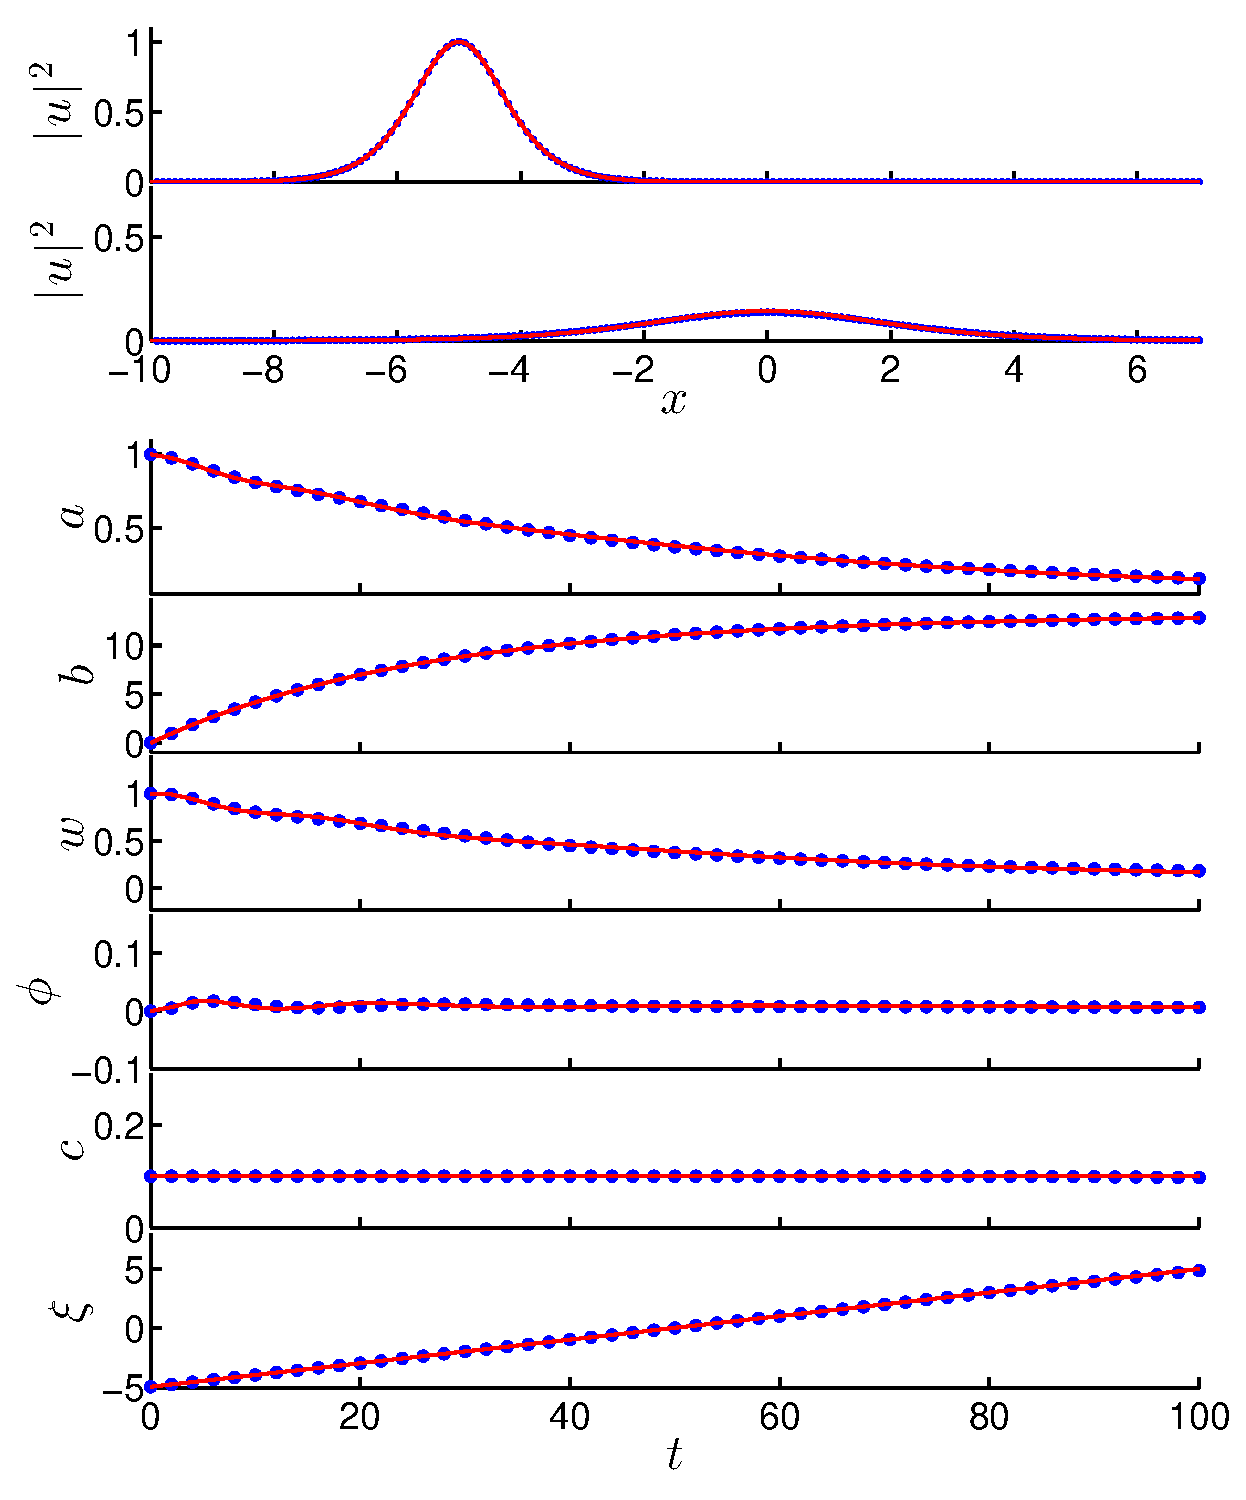
\includegraphics[width=0.8\textwidth]{fig1_LL_e001N.eps}}
  \rule{35em}{0.5pt}
  \caption[NLS with Linear Loss, $\epsilon = 0.01$]{Evolution of an NLS bright soliton under the presence of linear loss of strength $\epsilon=0.01$.  A bright soliton, as described by Eq.~(\ref{ansatz1}), is used as an initial condition with the parameters:  $a(0)=w(0)=1$, $c(0)=0.1$, $\xi(0) = -5$, and $b(0)=\phi(0)=0$.  The plots compare the NCVA approximations of Eq.~(\ref{eq:NCVALL}) (red lines) with the numerical NLS evolution of  Eq.~(\ref{eq:NLSLL}) (blue dots).  The top subpanel depicts the density $|u|^2$ at the initial time $(t=0)$.  The second subpanel depicts the density after the system is evolved for a total time of $t=1/\epsilon$.  The bottom six subpanels detail the evolution of the NCVA ansatz parameters $a$, $b$, $c$, $\xi$, $w$, and $\phi$ (red lines).  For the NLS evolution, the parameters are extracted by projecting the current solution into the NCVA ansatz using least squares fitting (blue dots).}
 \label{fig:Loss001}
\end{figure}


\begin{figure}[htbp]
  \centering
  \centerline{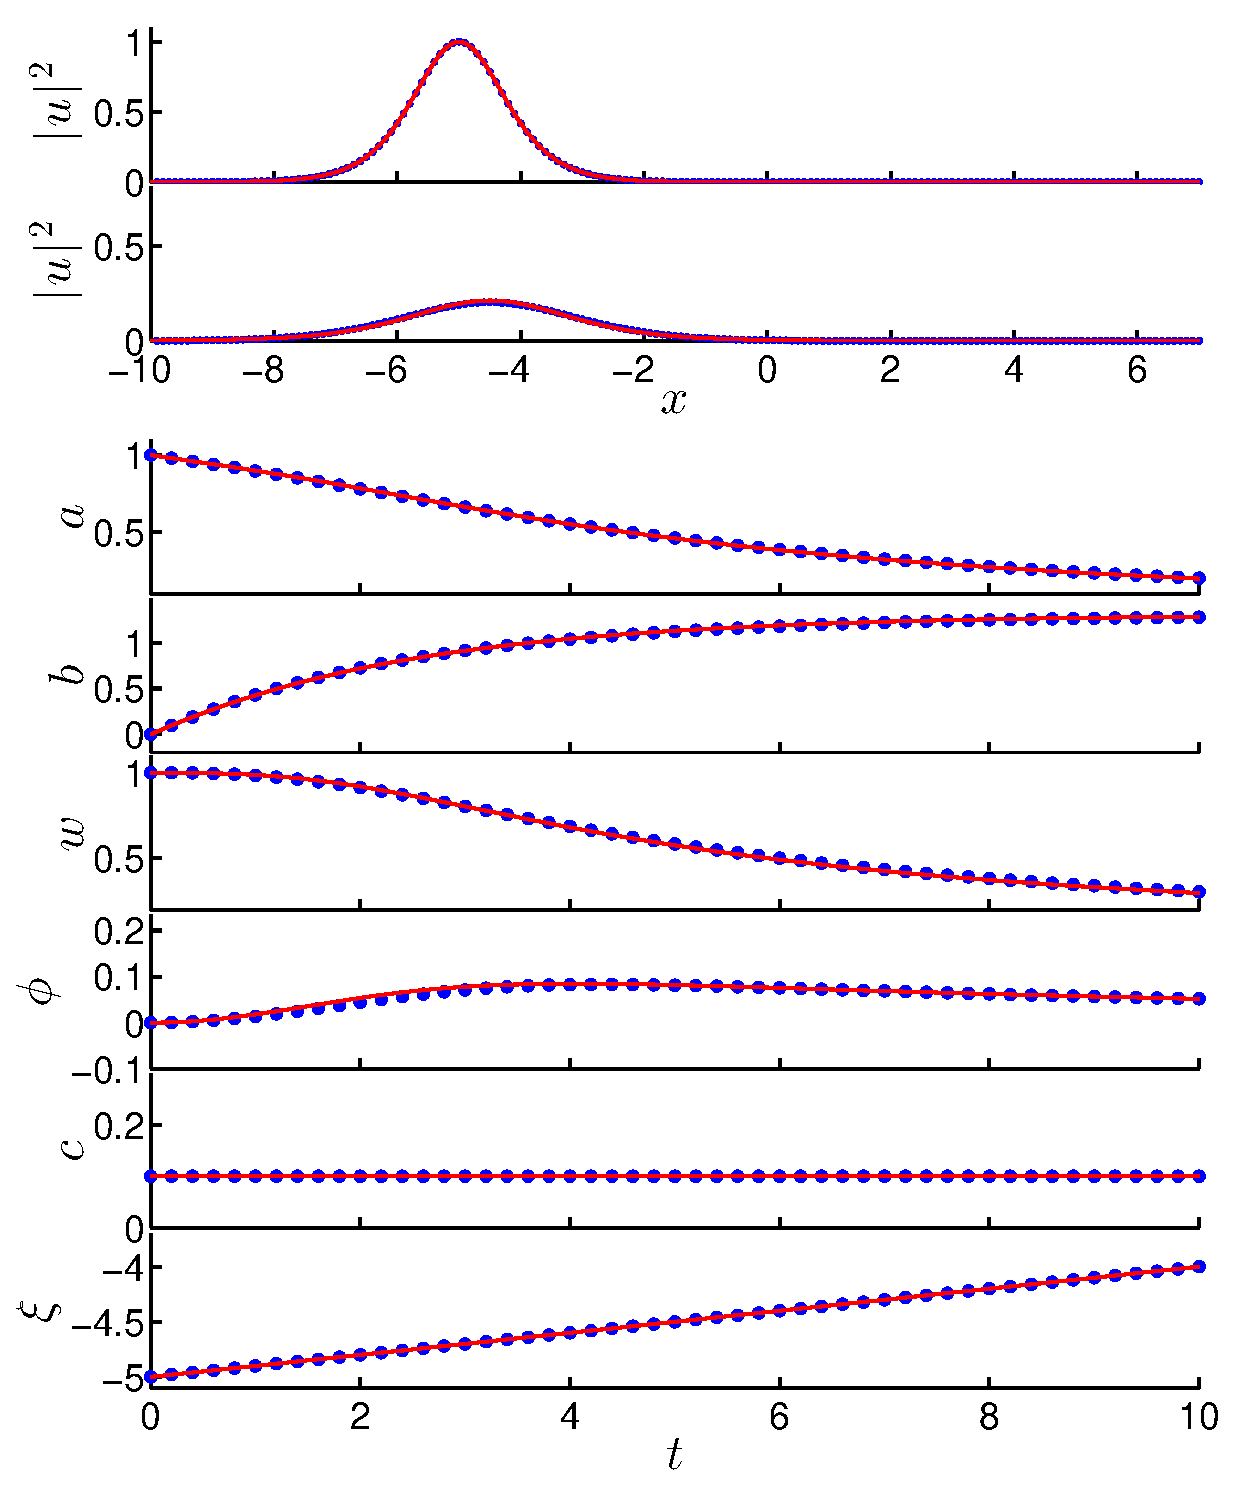
\includegraphics[width=0.8\textwidth]{fig2_LL_e01N.eps}}
  \rule{35em}{0.5pt}
  \caption[NLS with Linear Loss, $\epsilon = 0.1$]{Evolution of an NLS bright soliton under the presence of linear loss of strength $\epsilon=0.1$.  The NCVA results are obtained from Eq.~(\ref{eq:NCVALL}) (red lines) while the full numerical solution is obtained from Eq.~(\ref{eq:NLSLL}) (blue dots).  Same initial conditions and layout of panels as in the previous figure.}
 \label{fig:Loss01}
\end{figure}

\begin{figure}[htbp]
  \centering
  \centerline{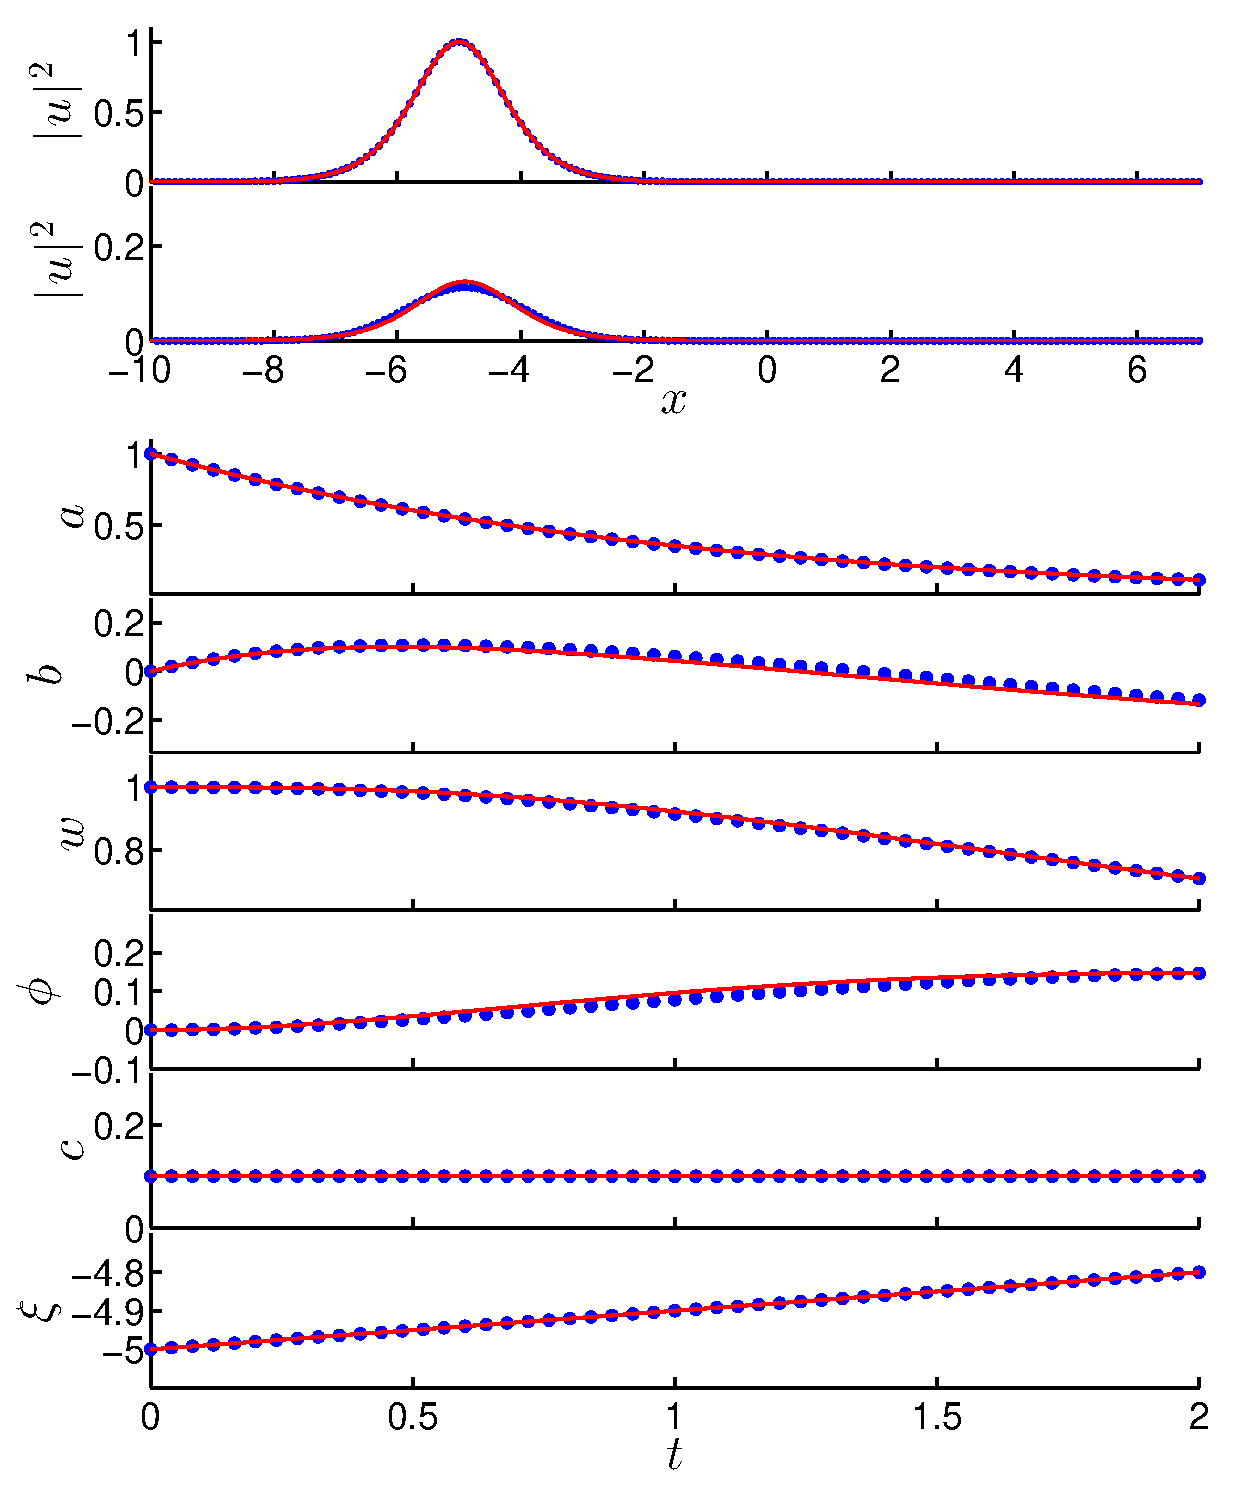
\includegraphics[width=0.8\textwidth]{Fig1b_LL_e1N.eps}}
  \rule{35em}{0.5pt}
  \caption[NLS with Linear Loss, $\epsilon = 1$]{Evolution of an NLS bright soliton under the presence of linear loss of strength $\epsilon=1$.  The NCVA results are obtained from Eq.~(\ref{eq:NCVALL}) (red lines) while the full numerical solution is obtained from Eq.~(\ref{eq:NLSLL}) (blue dots).  Same initial conditions and layout of panels as in previous figures.  The system is evolved for a total time of $t = 2/\epsilon$.}
   \label{fig:Loss1}
\end{figure}


%\begin{figure}[htbp]
%\centering
%\begin{subfigure}[t]{0.49\textwidth}
%  		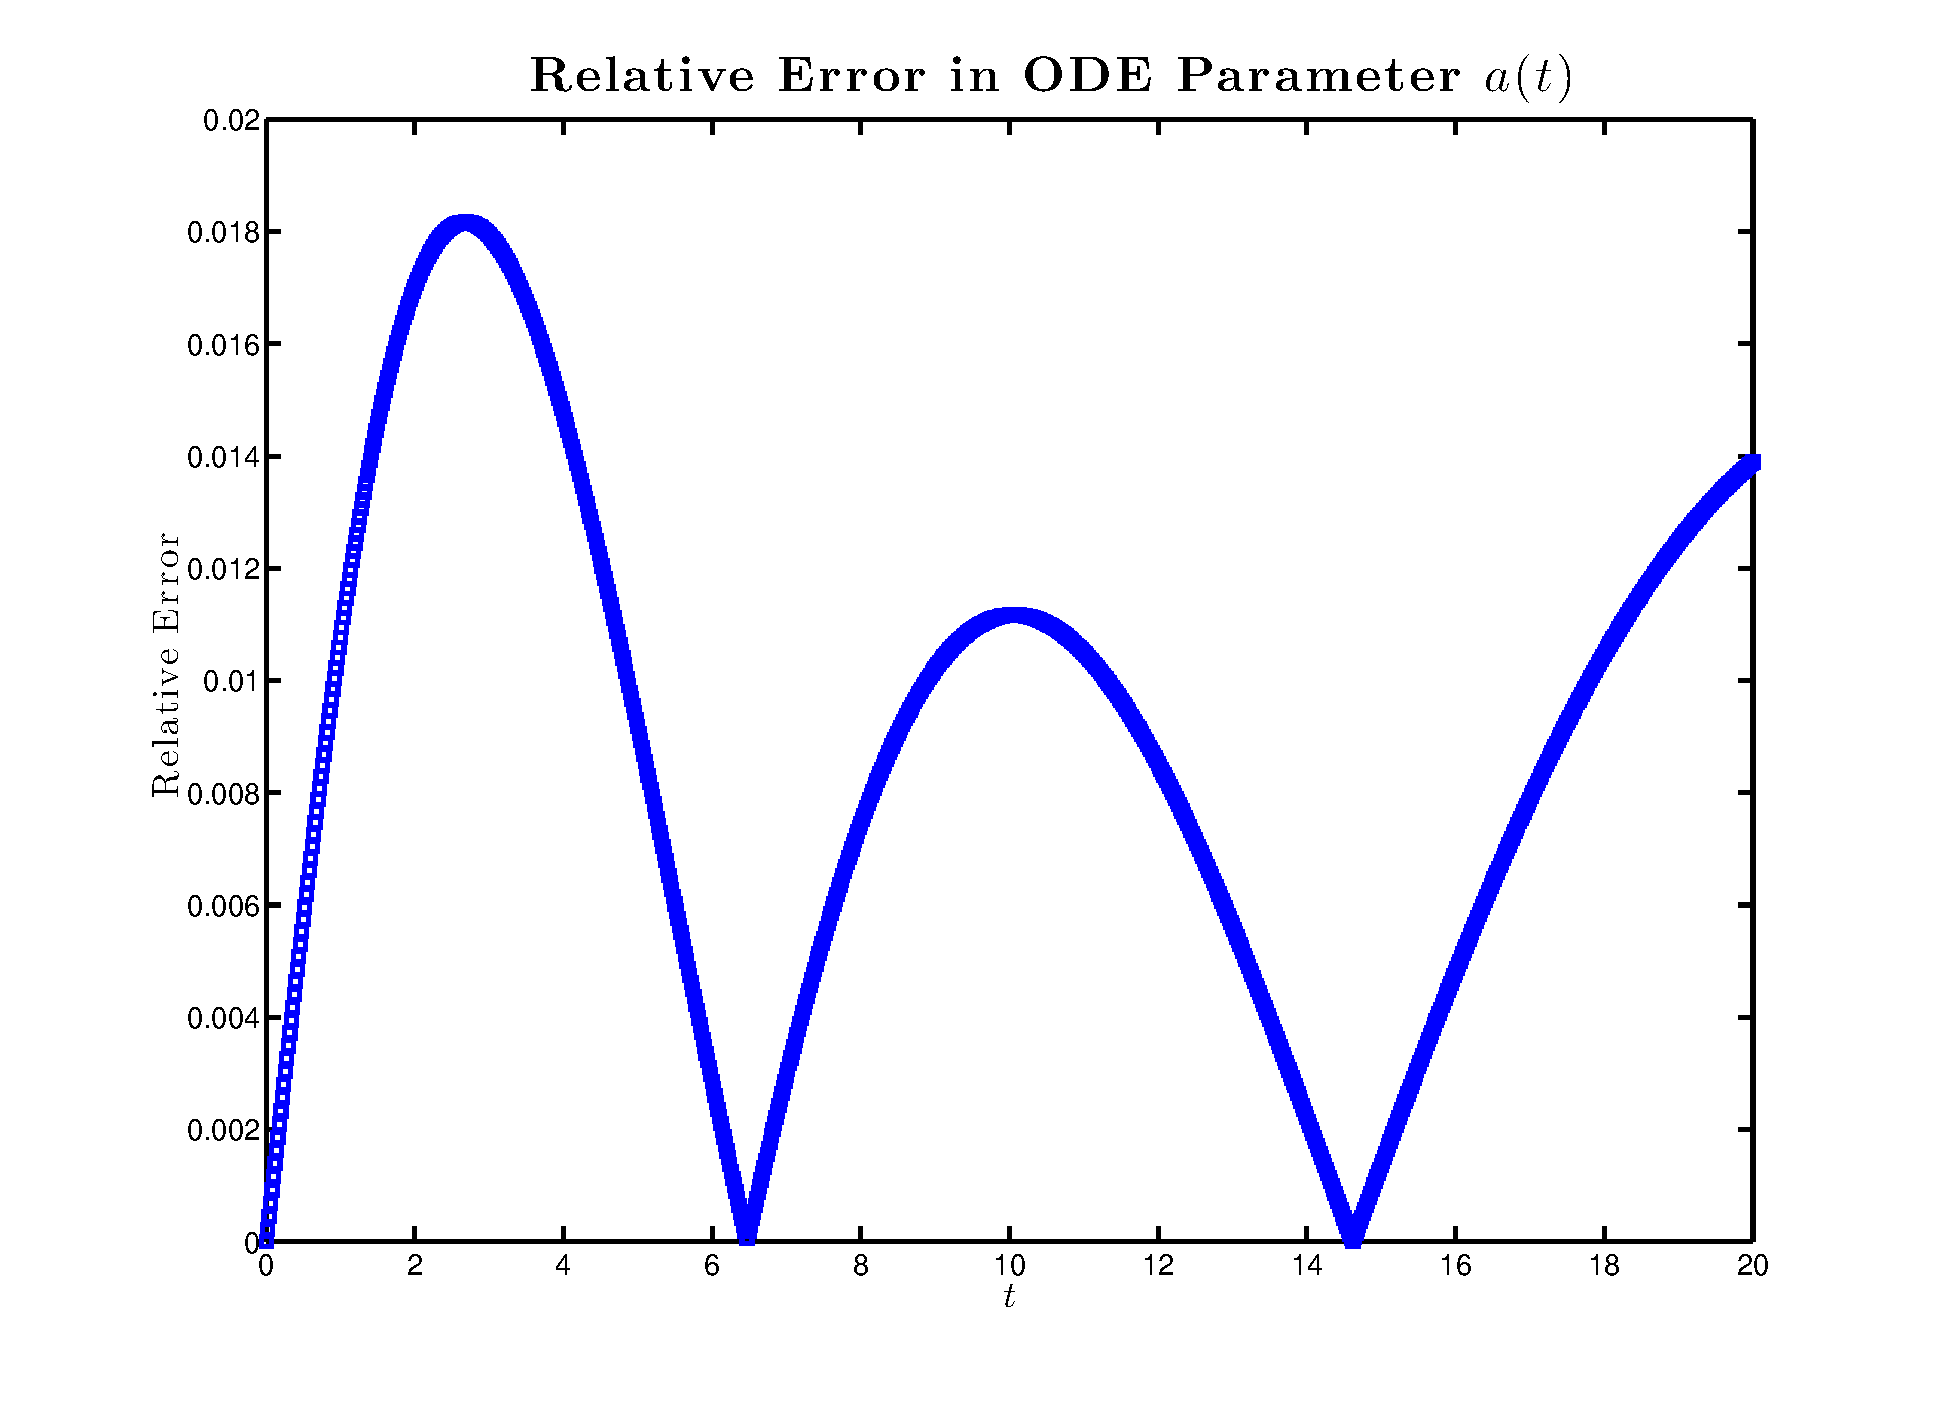
\includegraphics[width=\textwidth, height = \textwidth]{LL001relativeerror.eps}
%	         \caption{Relative error between NCVA and PDE parameter $a(t)$ values for $\epsilon=0.01$.}
%	         \label{fig:Loss001Err}
%	     \end{subfigure}
%  \begin{subfigure}[t]{0.49\textwidth}
%  		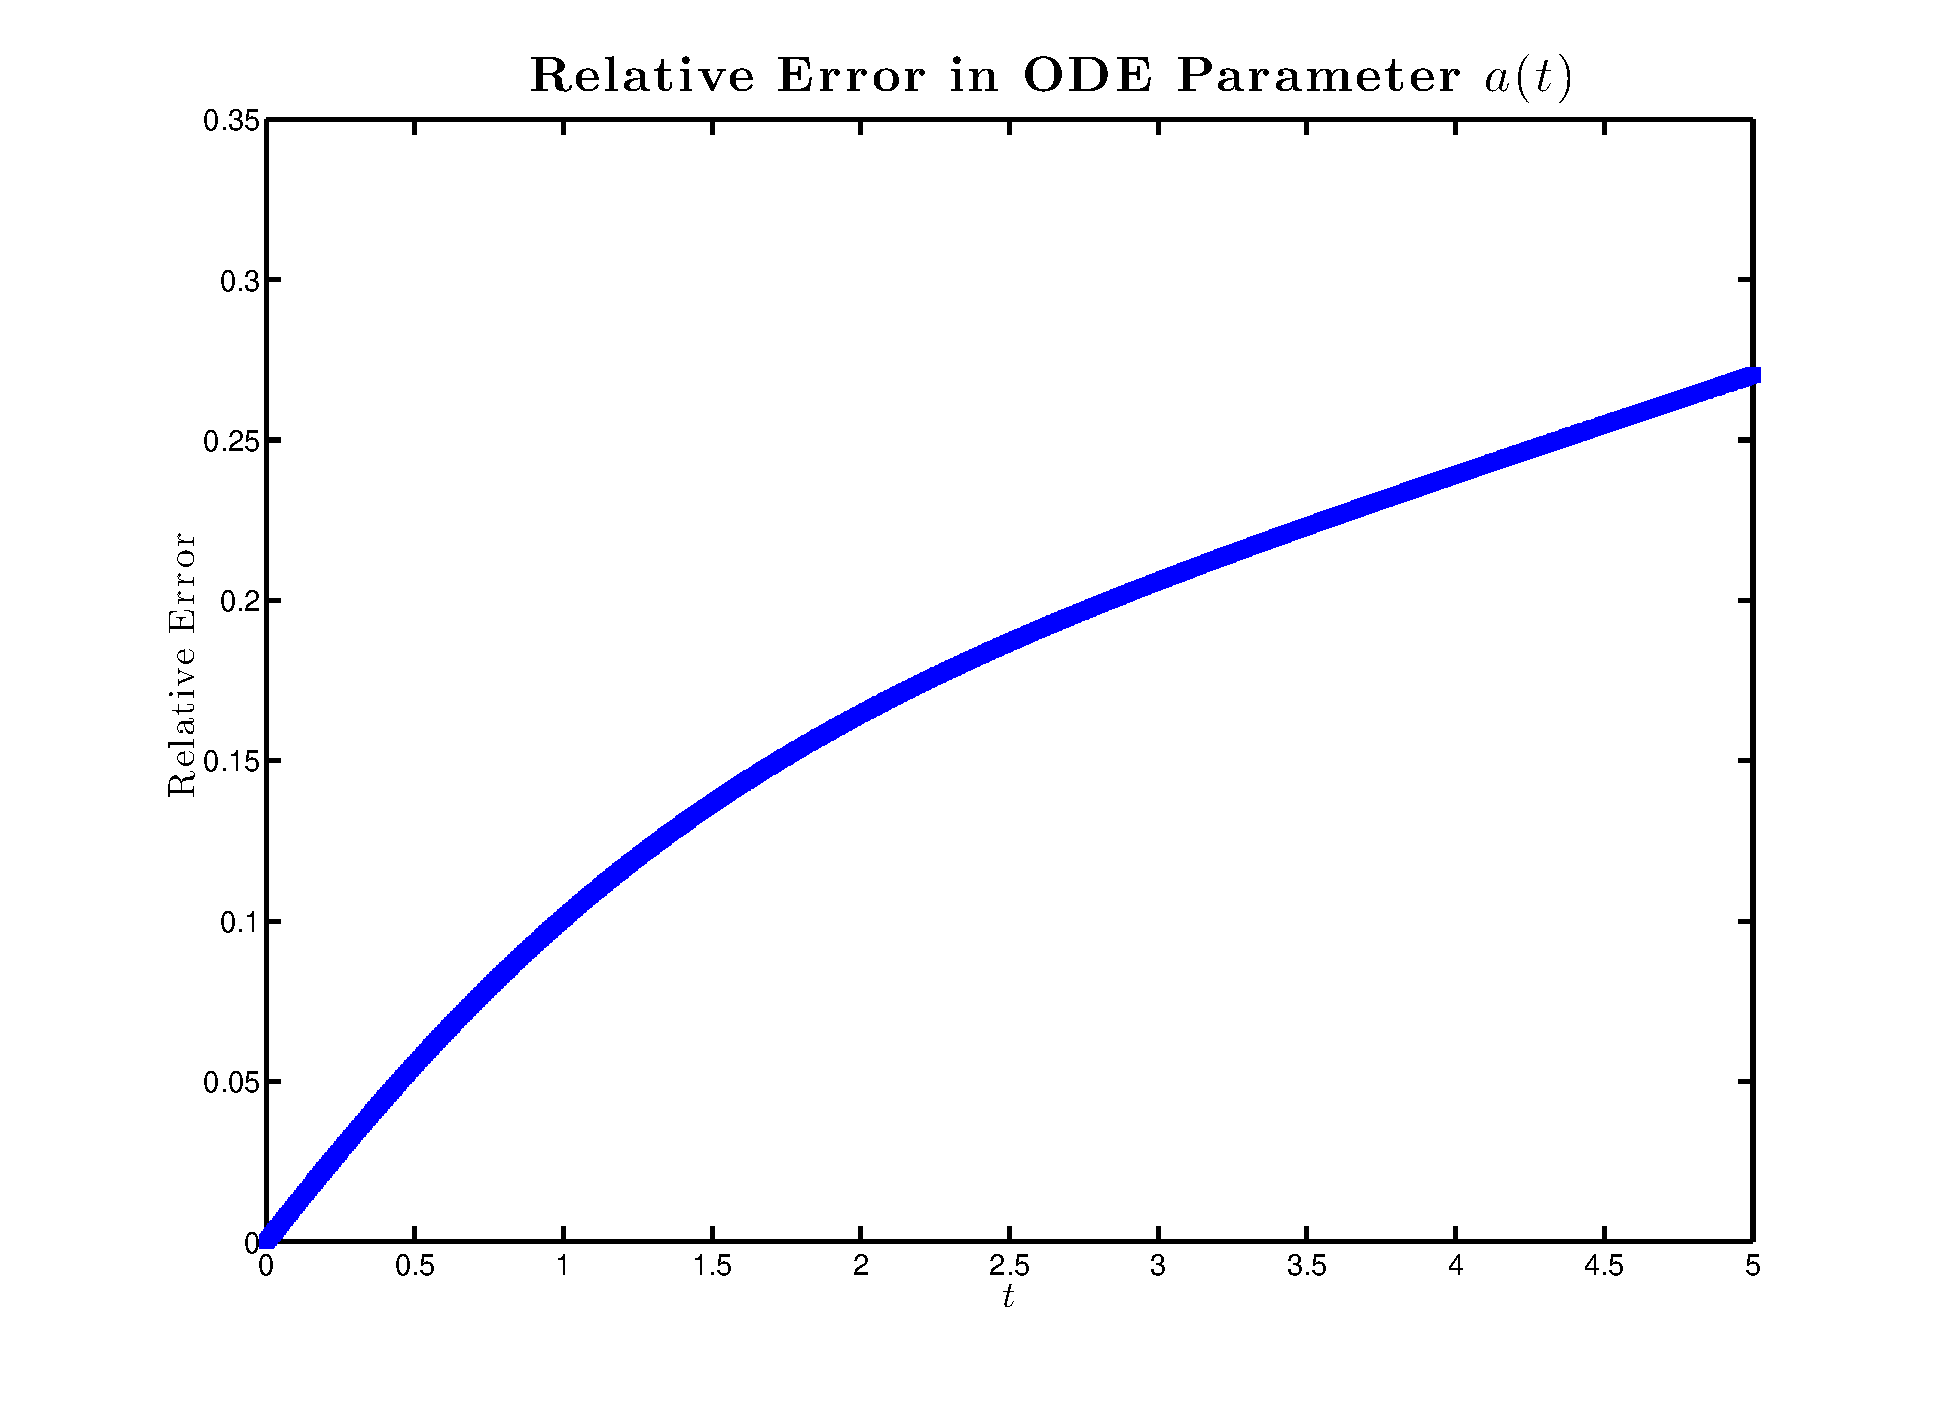
\includegraphics[width= \textwidth, height = \textwidth]{LL01relativeerror.eps}  
%	          \caption{Relative error between NCVA and PDE parameter $a(t)$ values for $\epsilon=0.1$.}
%	         \label{fig:Loss01Err}
%	    \end{subfigure} 
%  \rule{35em}{0.5pt}
%   \caption[Relative Error in Amplitude for NLS with Linear Loss]{{\bf NLS with Linear Loss:} Amplitude parameter $a(t)$ relative error for (A) $\epsilon=0.01$ and (B) $\epsilon=0.1$.}
%   \label{fig:LLossA}
%\end{figure}



%\begin{figure}[htbp]
%\centering
%\begin{subfigure}[t]{0.49\textwidth}
%  		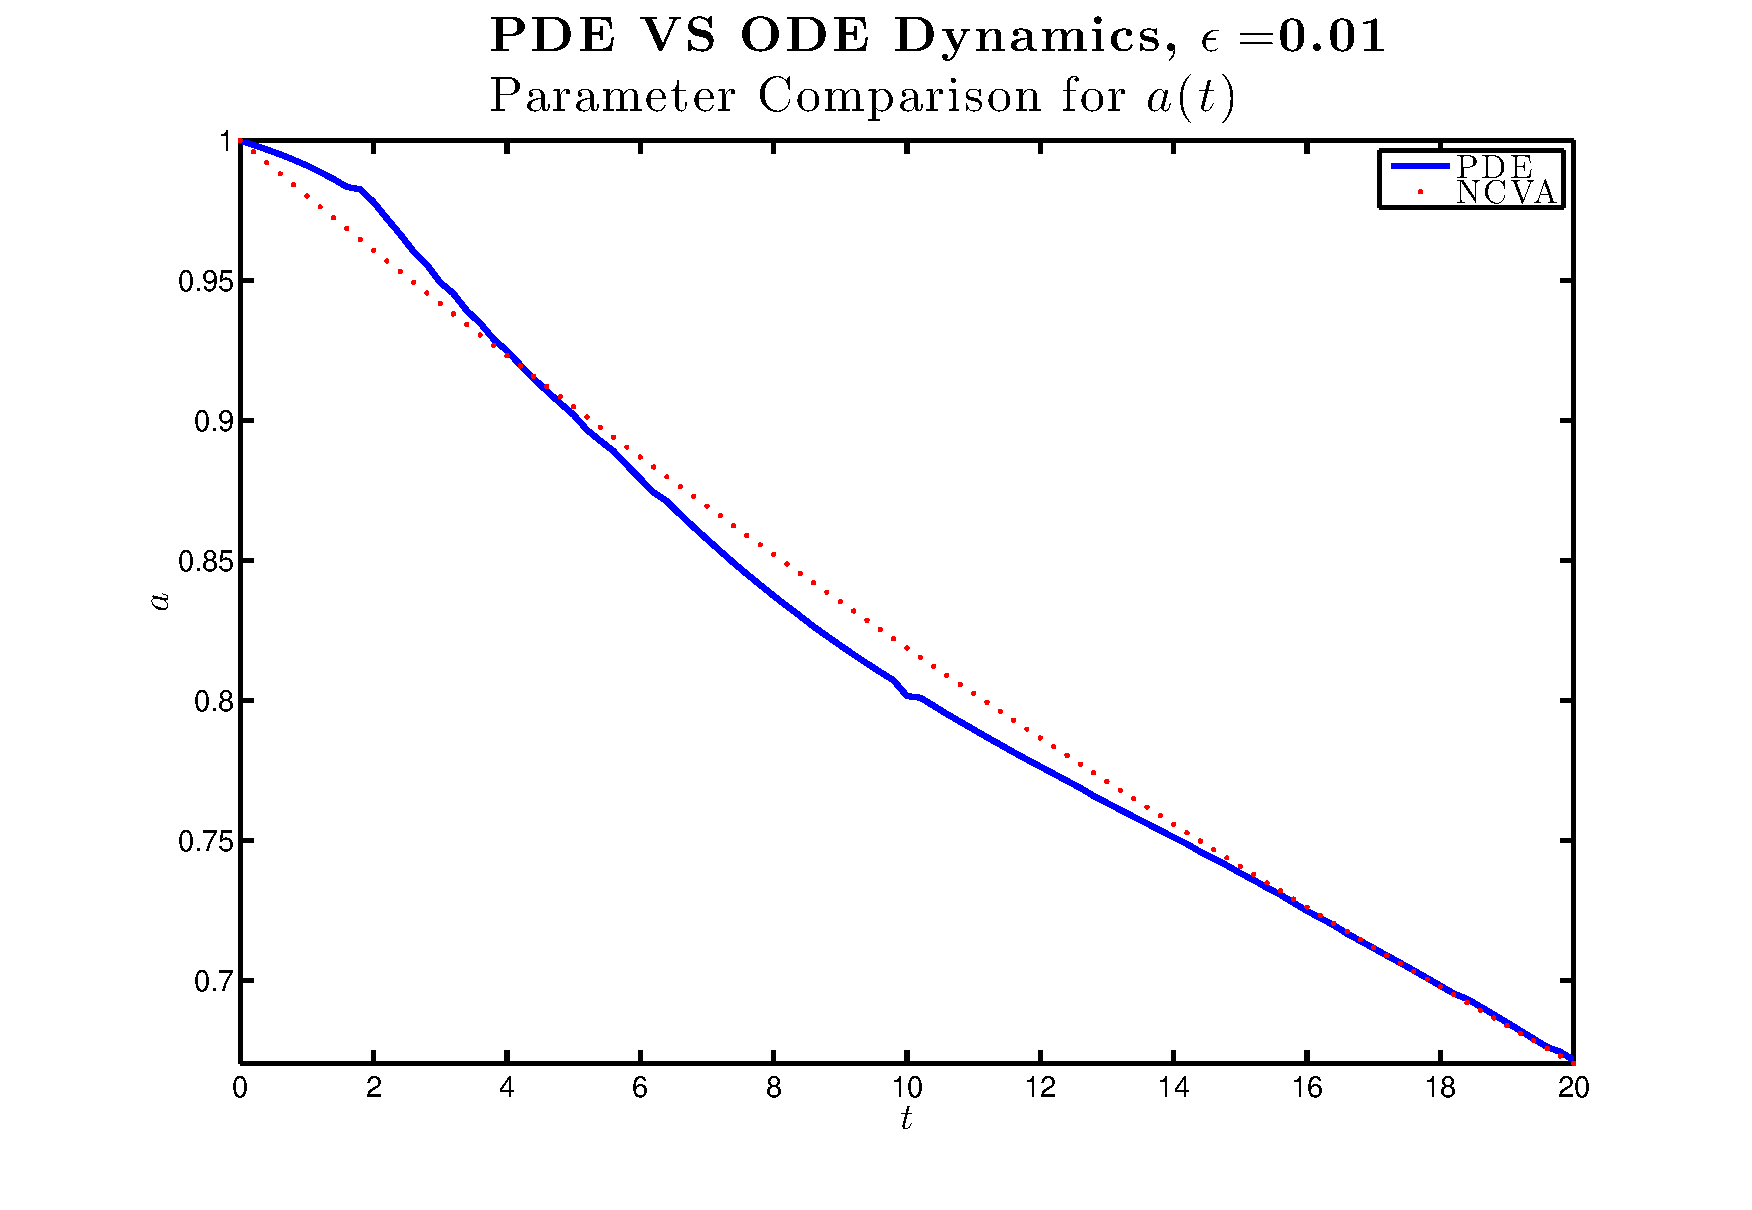
\includegraphics[width=\textwidth, height = \textwidth]{LLE001a.eps}
%	         \caption{Amplitude parameter comparison $a(t)$ between PDE and NCVA solutions.}
%	         \label{fig:Loss001a}
%	     \end{subfigure}
%  \begin{subfigure}[t]{0.49\textwidth}
%  		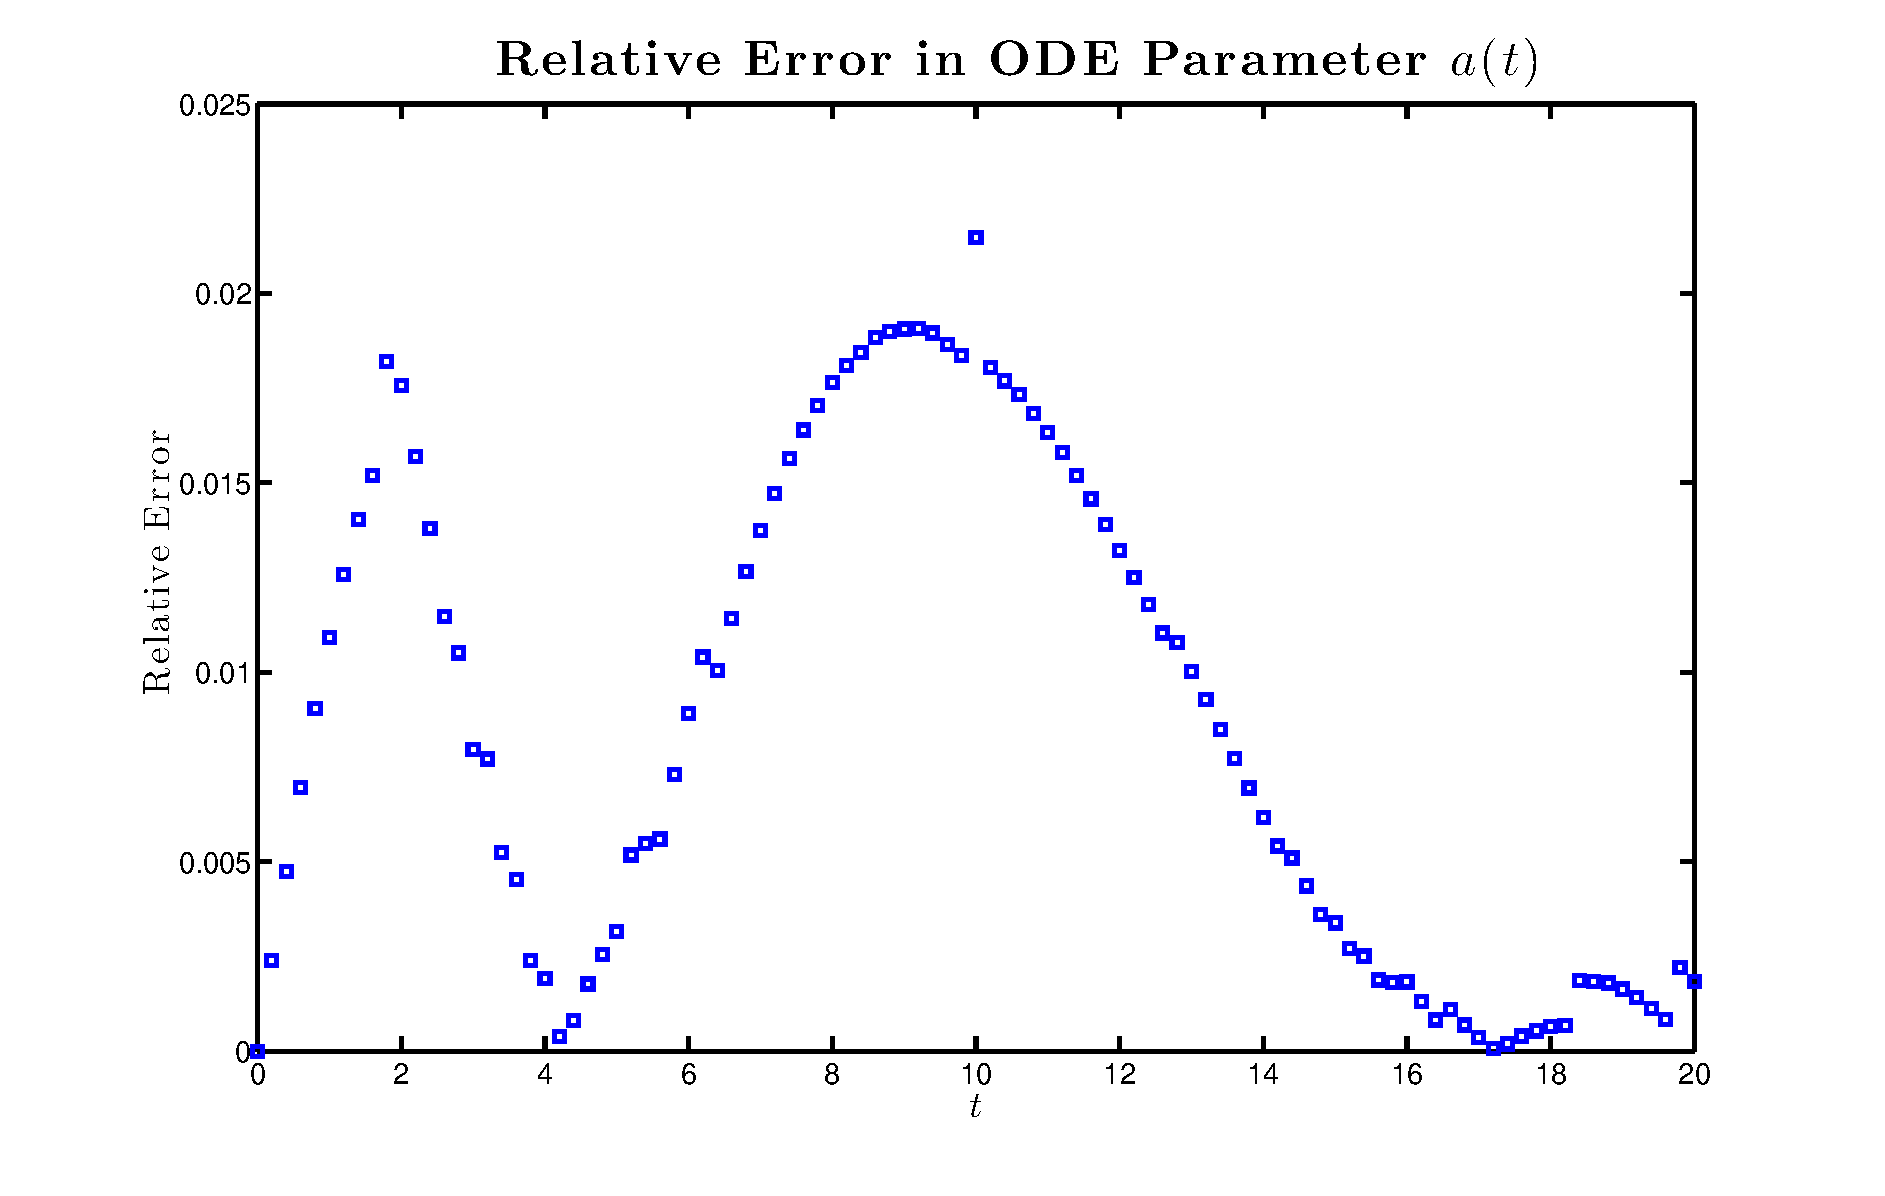
\includegraphics[width= \textwidth, height = \textwidth]{LLE001relativeError.eps}  
%	          \caption{Relative error between NCVA and PDE parameter $a(t)$ values.}
%	         \label{fig:Loss001Err}
%	    \end{subfigure} 
%  \rule{35em}{0.5pt}
%   \caption[NLS with Linear Loss, $\epsilon = 0.01$ Amplitude Comparison and Relative Error]{{\bf NLS with Linear Loss:} Amplitude parameter $a(t)$ ansatz comparisons and relative error for $\epsilon=0.01$.}
%   \label{fig:LLossA}
%\end{figure}
%
%
%\begin{figure}[htbp]
%\begin{subfigure}[b]{0.5\textwidth}
%  		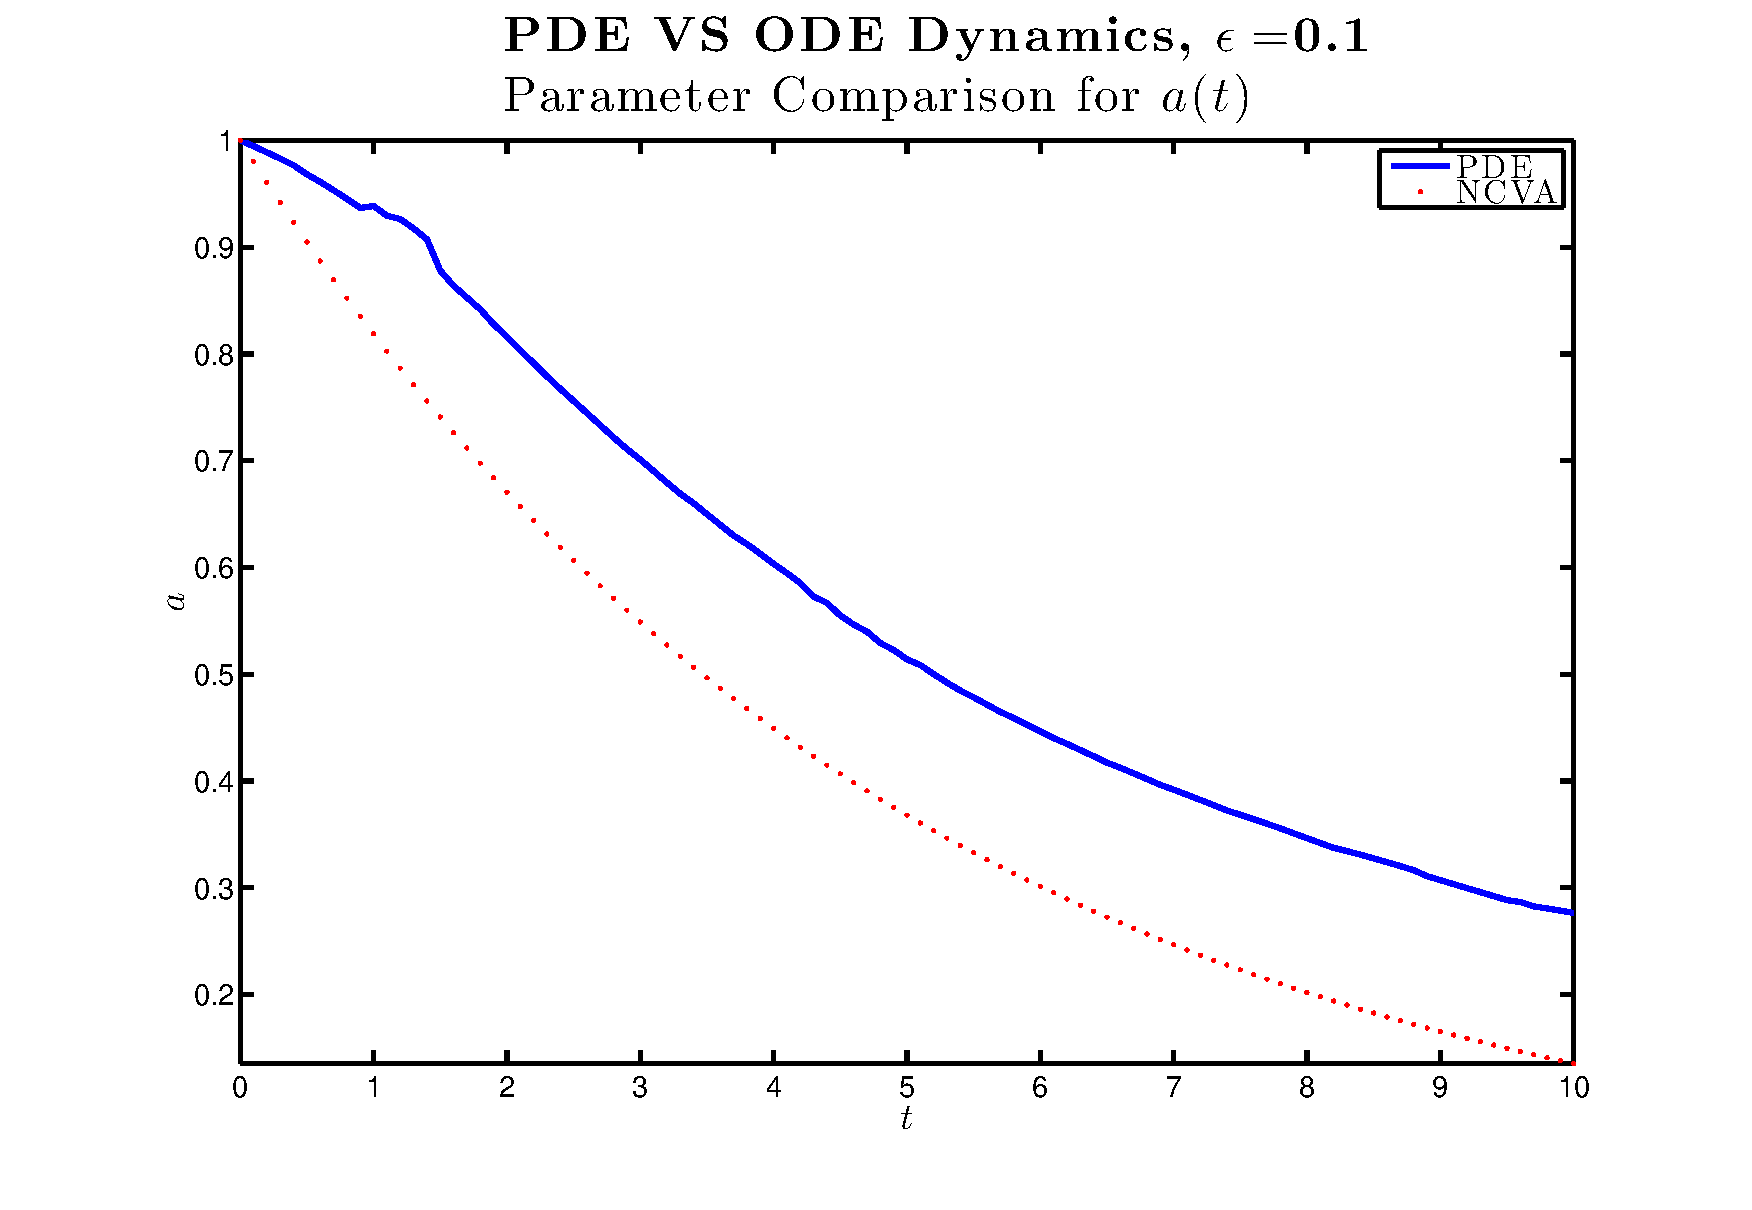
\includegraphics[width=\textwidth, height = \textwidth]{LLE01a.eps}
%	         \caption{Amplitude parameter comparison $a(t)$ between PDE and NCVA solutions.}
%	         \label{fig:Loss01a}
%	     \end{subfigure}
%  \begin{subfigure}[b]{0.5\textwidth}
%  		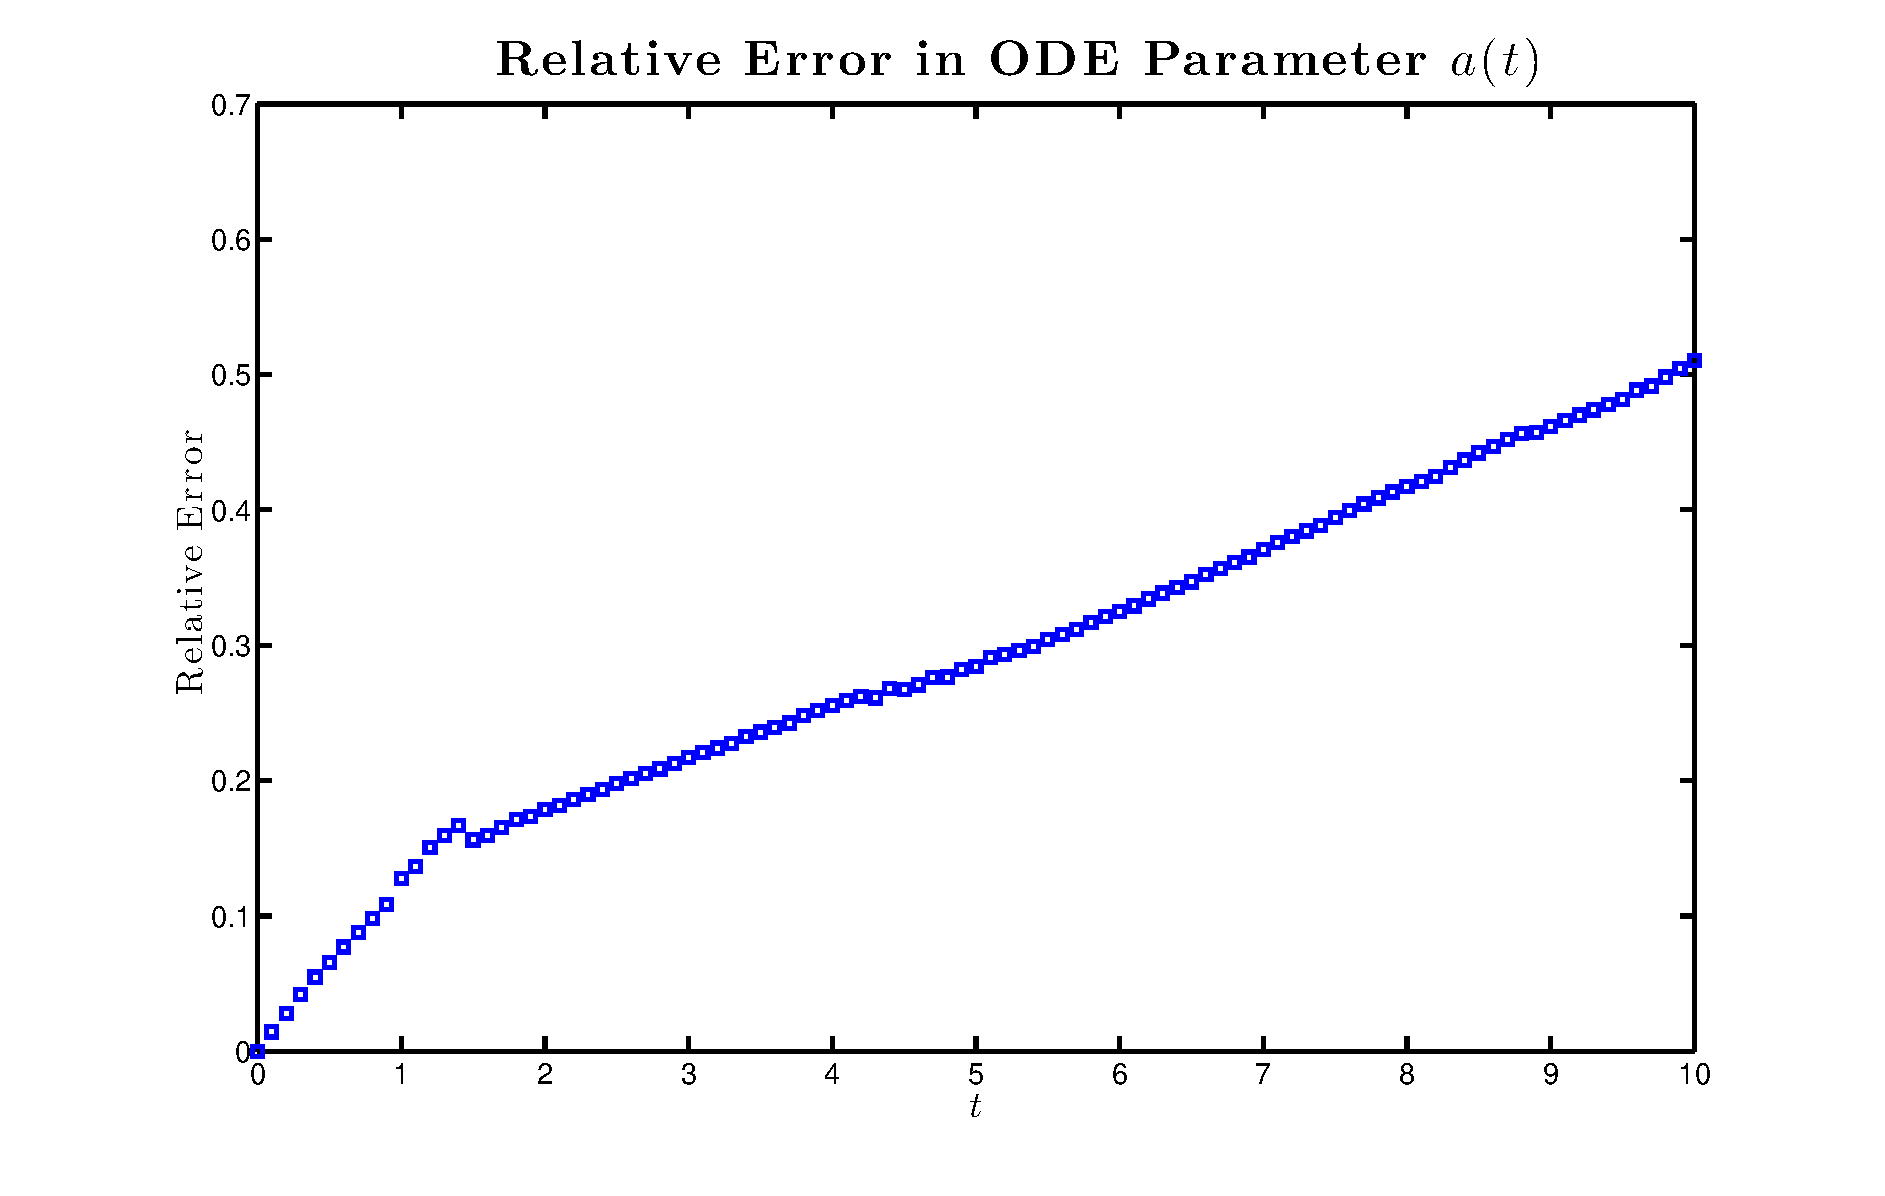
\includegraphics[width= \textwidth, height = \textwidth]{LLE01relativeError.eps}  
%	          \caption{Relative error between NCVA and PDE parameter $a(t)$ values.}
%	         \label{fig:Loss01Err}
%	    \end{subfigure} 
%  \rule{35em}{0.5pt}
%   \caption[NLS with Linear Loss, $\epsilon = 0.1$ Height Comparison and Relative Error]{{\bf NLS with Linear Loss:} Amplitude parameter $a(t)$ ansatz comparisons and relative error for $\epsilon=0.1$.}
%   \label{fig:LLossA2}
%\end{figure}

\clearpage
%%%% Section NLS with Density Dependent Loss %%%%%%%%%%%
\setstretch{1.3}
\section[Nonlinear Schr\"{o}dinger Equation with Density Dependent Loss]{NLS Equation with Density Dependent Loss}
\label{section:DDL}

\setstretch{2}
In the second dynamical system example, we use the attractive NLS equation with a density dependent (nonlinear) loss term of strength $\epsilon$:
\begin{align}
iu_t + \frac{1}{2} u_{xx} + |u|^2 u = -i  \epsilon  |u|^2 u. 
\label{eq:NLSDD}
\end{align}
The Lagrangian corresponding to the conservative problem ($\epsilon = 0$) is the same as Eq.~(\ref{eq:ConservativeL}).
% given by:
%\begin{align}
%\mathcal{L} = \frac{i}{2} \Bigg( u \frac{\partial u^*}{\partial t} -u^* \frac{\partial u}{\partial t} \Bigg) + \frac{1}{2} \Bigg| \frac{\partial u}{\partial x} \Bigg|^2  - \frac{1}{2} | u|^4.
%\end{align}
We again use the bright soliton ansatz Eq.~(\ref{ansatz1})
%\begin{align}
%u_A(x,t; \vec{p}) = a \, \mathrm{sech}[w(x-\xi)] \, \exp [i(b(x-\xi)^2+ c(x-\xi)+\phi)],
%\label{ansatz1}
%\end{align}
with a vector of time-dependent ansatz parameters given by $\vec{p} = (a, w, \xi, c, b, \phi)$.
% with arbitrary height $a$, inverse width $w$, center position $\xi$, speed $c$, chirp $b$, and phase $\phi$. 

%\subsection{Perturbed Variational Approximation}
%In the perturbed and modified Kantorovitch variational approximation methods the non-conservative term is given by 
%\begin{align}
%\mathcal{P} = \epsilon \mathcal{Q} = - i \epsilon |u|^2 u,
%\end{align}
%and the two solutions are equivalent.  
%%According to Cerda's~\cite{Cerda} method the non-conservative term is described as
%%\begin{align}
%%Q = -i\epsilon |u|^2 u,
%%\end{align}
%%and the two solutions are equivalent.
%From the modified Kantorovitch method and the perturbed variational approximation it is straightforward to obtain a system of six coupled ODEs for the ansatz parameters:
%%\begin{align} \begin{cases}
%%2 \dot{b} - a^2 - 2c\dot{\xi} + c^2 = 0, \\
%%-2\dot{a} = \frac{8}{3} \epsilon a^3, \\
%%-2\dot{\xi} a + 2ac = 0, \\
%%2 \dot{a} c + 2 a \dot{c} = -\frac{8}{3} \epsilon a^3 c. 
%%\end{cases} \end{align} 
%%The four equations are solved simultaneously to find the following system of ODEs for the NLS with density dependent loss: 
%{\setstretch{1.3} 
%\begin{align}\begin{cases}
% \dot{a} = - \frac{2}{3} \epsilon a^3   - a b - \frac{2}{\pi^2} \epsilon a^3, \\[1.0ex]
%\dot{b}  = \frac{2}{\pi^2}w^4 - \frac{2}{\pi^2}a^2 w^2 - 2 b^2, \\[1.0ex]
%\dot{c} = 0 , \\[1.0ex]
%\dot{\xi} = c, \\[1.0ex]
%\dot{w} = -2bw - \frac{4}{\pi^2} \epsilon a^2 w, \\[1.0ex]
%\dot{\phi} = \frac{5}{6} a^2 - \frac{1}{3} w^2 + \frac{1}{2} c^2,
%\end{cases} \label{eq:PVADD} \end{align}}
%\vskip -5cm

\subsection{Non-conservative Variational Approximation} \label{section:DD}
In the NCVA framework, the $\bar{u}_1$ and $\bar{u}_2$ ans\"{a}tze are defined as in Eqs.~(\ref{eq:psi1}) and (\ref{eq:psi2}).
%\begin{align}
%u_1 &= a_1 \mathrm{sech}(a_1(x-\xi_1))e^{i(c_1 (x-\xi_1)+b_1)}, \\
%u_2 &= a_2 \mathrm{sech}(a_2(x-\xi_2))e^{i(c_2 (x-\xi_2)+b_2)}.
%\end{align}
According to the non-conservative variational method the Lagrangian is $\mathcal{L}_t = \mathcal{L}_1 - \mathcal{L}_2 + \mathcal{R}$ where 
\begin{align}
\mathcal{L}_1 &= \frac{i}{2} \Big(\bar{u}_1 \bar{u}_{1,t}^* - \bar{u}_1^* \bar{u}_{1,t}\Big) + \frac{1}{2} |\bar{u}_{1,x}|^2 - \frac{1}{2}|\bar{u}_1|^4, \\
\mathcal{L}_2 &= \frac{i}{2} \Big(\bar{u}_2 \bar{u}_{2,t}^* - \bar{u}_2^* \bar{u}_{2,t}\Big) + \frac{1}{2} |\bar{u}_{2,x}|^2 - \frac{1}{2}|\bar{u}_2|^4, \\
\mathcal{P} \bar{u}_-^* &=  i\epsilon  \bar{u}_+ \bar{u}_+^* \bar{u}_+\bar{u}_-^* =  i \epsilon  \frac{(\bar{u}_1 + \bar{u}_2)}{2}\frac{(\bar{u}_1^* + \bar{u}_2^*)}{2}\frac{(\bar{u}_1 + \bar{u}_2)}{2}(\bar{u}_1 - \bar{u}_2)^*, \\
\mathcal{R} & =  i\epsilon ( \bar{u}_+ \bar{u}_+^* \bar{u}_+\bar{u}_-^* -  \bar{u}_+ \bar{u}_+^* \bar{u}_-\bar{u}_+^*).  
\end{align}
Plugging the ans\"{a}tze into $\mathcal{L}_1$ and $\mathcal{L}_2$ and integrating gives $\bar{L}_1$ and $\bar{L}_2$ of the same form as Eq.~({\ref{eq:intLi}).
%\begin{align}
%L_1 =& a_1^2 \mathrm{sech}^2(a_1(x-\xi_1))[\dot{c}_1 (x-\xi_1)-c_1\dot{\xi}_1 + \dot{b}_1] + \frac{1}{2}a_1^4 \mathrm{sech}^2(a_1(x-\xi_1))\mathrm{tanh}^2(a_1(x-\xi_1)) \nonumber \\
%&+\frac{1}{2}a_1^2c_1^2 \mathrm{sech}^2(a_1(x-\xi_1))-\frac{1}{2}a_1^4 \mathrm{sech}^4(a_1(x-\xi_1)), \\
%L_2 =& a_2^2 \mathrm{sech}^2(a_2(x-\xi_2))[\dot{c}_2 (x-\xi_2)-c_2\dot{\xi}_2 + \dot{b}_2] + \frac{1}{2}a_2^4 \mathrm{sech}^2(a_2(x-\xi_2))\mathrm{tanh}^2(a_2(x-\xi_2)) \nonumber \\
%&+\frac{1}{2}a_2^2c_2^2 \mathrm{sech}^2(a_2(x-\xi_2))-\frac{1}{2}a_2^4 \mathrm{sech}^4(a_2(x-\xi_2)).  
%\end{align}
%Next we find $\bar{L} = \int\mathscr{L}dx = \int L_1 dx - \int L_2 dx + \int R dx$, which for $L_1$ and $L_2$ is the same as with the conservative variational approximation.  The first two integrals are
%\begin{align}
%\int_{-\infty}^{\infty} L_1 dx &= 2\dot{b}_1 a_1 - \frac{1}{3}a_1^3 + c_1^2 a_1 - 2c_1 \dot{\xi}_1 a_1,  \\
%\int_{-\infty}^{\infty} L_2 dx &= 2\dot{b}_2 a_2 - \frac{1}{3}a_2^3 + c_2^2 a_2 - 2c_2 \dot{\xi}_2 a_2.
%\end{align}
%The solution for the non-conservative density dependent loss term in the effective Lagrangian is an integral of the form
%\begin{align}
%\int_{-\infty}^{\infty} \mathcal{R} dx &=   \\
% &  \frac{i}{4} \epsilon  \int & \Big( |u_1|^2( u_2u_1^* - u_2^* u_1) +  |u_2|^2( u_2u_1^* - u_2^* u_1)  + u_2u_2 u_1^*u_1^* - u_1u_1u_2^*u_2^*\Big)dx. \nonumber
%\end{align}
For the non-conservative terms, we take derivatives with respect to $p_-$ at the physical limit ($\mathrm{PL}$) and then integrate: 
\begin{align} 
\bar{R} = &  \int_{-\infty}^{\infty} \bar{\mathcal{R}} dx \nonumber \\
%\int \Big[ \frac{\partial R}{\partial p_-} \Big]_{\mathrm{PL}} dx  \nonumber \\ 
=&  \frac{i }{4} \epsilon \int \Big[ \frac{\partial}{\partial p_-} \Big(|u_1|^2( u_2u_1^* - u_2^* u_1) +  |u_2|^2( u_2u_1^* - u_2^* u_1)  + u_2u_2 u_1^*u_1^* - u_1u_1u_2^*u_2^*\Big) \Big]_{\mathrm{PL}} dx.   
\end{align}
%Putting everything back together we obtain the modified Euler-Lagrange equations:
%\begin{align}
%\frac{\partial \bar{L}}{\partial p} - \frac{d}{dt} \Bigg( \frac{\partial \bar{L} }{\partial\dot{p}}\Bigg) + \int_{-\infty}^{\infty} \Big[ \frac{\partial \bar{\mathcal{R}}}{\partial p_-} \Big]_{\mathrm{PL}} dx = 0. 
%\end{align}
Therefore, the total effective Lagrangian, $\bar{L} = \bar{L}_1 - \bar{L}_2 + \bar{R}$ is given by:
\begin{align} 
\bar{L} =& 2\frac{a_1^2  \dot{\phi}_1}{w_1}+\frac{a_1^2 c_1^2}{w_1} - 2 \frac{a_1^2 c_1 \dot{\xi}_1}{w_1} - \frac{2}{3} \frac{a_1^4}{w_1} +\frac{1}{3} a_1^2 w_1 + \frac{\pi^2}{3} \frac{ a_1^2 b_1^2}{w_1^3} + \frac{\pi^2}{6} \frac{a_1^2 \dot{b}_1}{w_1^3}  \nonumber \\
&- 2\frac{a_2^2  \dot{\phi}_2}{w_2}-\frac{a_2^2 c_2^2}{w_2} + 2 \frac{a_2^2 c_2 \dot{\xi}_2}{w_2} + \frac{2}{3} \frac{a_2^4}{w_2} -\frac{1}{3} a_2^2 w_2 - \frac{\pi^2}{3} \frac{ a_2^2 b_2^2}{w_2^3} - \frac{\pi^2}{6} \frac{a_2^2 \dot{b}_2}{w_2^3} \nonumber \\
&+ \frac{i}{4} \epsilon \int \Big[ \frac{\partial}{\partial p_-} \Big(|u_1|^2( u_2u_1^* - u_2^* u_1) +  |u_2|^2( u_2u_1^* - u_2^* u_1)  + u_2u_2 u_1^*u_1^* - u_1u_1u_2^*u_2^*\Big) \Big]_{\mathrm{PL}} dx . 
\end{align}

For all the parameters, we substitute the $\pm$ coordinates into the expression for the total effective Lagrangian $\bar{L}$.
% = \bar{L}_{C} + \bar{L}_{NC}$ where $\bar{L}_C$ is the same as in Eq.~(\ref{barLC}) and :
%\begin{align} 
%\bar{L} =& 2\Bigg[  \Bigg(\frac{2\dot{b}_+ +\dot{ b}_-}{2}\Bigg)\Bigg(\frac{2a_+ + a_-}{2}\Bigg) - \Bigg(\frac{2\dot{b}_+ - \dot{b}_-}{2}\Bigg)\Bigg(\frac{2a_+ - a_-}{2}\Bigg) \Bigg] \nonumber \\
%&+ \frac{1}{3} \Bigg[ \Bigg(\frac{2a_+ - a_-}{2} \Bigg)^3 - \Bigg(\frac{2a_+ - a_-}{2} \Bigg)^3   \Bigg] \nonumber \\
%&+ \Bigg[ \Bigg(\frac{2c_+ + c_-}{2} \Bigg)^2\Bigg(\frac{2a_+ + a_-}{2} \Bigg) -    \Bigg(\frac{2c_+ - c_-}{2} \Bigg)^2\Bigg(\frac{2a_+ -a_-}{2} \Bigg)  \Bigg] \nonumber \\
%&+ 2 \Bigg[\Bigg(\frac{2c_+ - c_-}{2} \Bigg)\Bigg(\frac{2\dot{\xi}_+ - \dot{\xi}_-}{2} \Bigg)\Bigg(\frac{2a_+ + a_-}{2} \Bigg) - \Bigg(\frac{2c_+ + c_-}{2} \Bigg)\Bigg(\frac{2\dot{\xi}_+ + \dot{\xi}_-}{2} \Bigg)\Bigg(\frac{2a_+ + a_-}{2} \Bigg) \Bigg]  \nonumber \\
%\bar{L}_{NC} =   \frac{i}{4} \epsilon \int \Big[ \frac{\partial}{\partial p_-} \Big(|u_1|^2( u_2u_1^* - u_2^* u_1) +  |u_2|^2( u_2u_1^* - u_2^* u_1)  + u_2u_2 u_1^*u_1^* - u_1u_1u_2^*u_2^*\Big) \Big]_{\mathrm{PL}} dx. 
%\end{align} 
From the $\bar{L}_1$ and $\bar{L}_2$ conservative terms we recover the standard soliton evolution equations [see Eq.~(\ref{eq:CODEsNLS})], so we just need to obtain the non-conservative ones.
%{\textit i.e.} variational approximation of NLS with the following equations of motion (ODEs):
%\[\begin{cases}
%\dot{a}  = 0 \\
%\dot{b}  = \frac{1}{2}a^2 + \frac{1}{2} c^2 \\
%\dot{c} = 0  \\
%\dot{\xi} = c
%\end{cases}\] 
From the non-conservative term $\bar{R}$, we expand in the $\pm$ coordinate systems and find the integrals:
\begin{eqnarray}
\int_{-\infty}^{\infty} \left[ \frac{\partial  \bar{\mathcal{R}}}{\partial a_-} \right]_{\rm PL} dx &=& 0,  \nonumber  \\
\int_{-\infty}^{\infty} \left[ \frac{\partial  \bar{\mathcal{R}}}{\partial b_-} \right]_{\rm PL} dx &=& -\frac{2\pi^2\epsilon}{9}  \frac{a^4}{w^3} + \frac{4\epsilon}{3} \frac{a^4}{w^3}, \nonumber \\
\int_{-\infty}^{\infty} \left[ \frac{\partial  \bar{\mathcal{R}}}{\partial c_-} \right]_{\rm PL} dx &=& 0, \nonumber \\
\int_{-\infty}^{\infty} \left[ \frac{\partial  \bar{\mathcal{R}}}{\partial \xi_-} \right]_{\rm PL} dx &=&  \frac{8\epsilon}{3}   \frac{a^4 c }{w},\nonumber \\
\int_{-\infty}^{\infty} \left[ \frac{\partial  \bar{\mathcal{R}}}{\partial w_-} \right]_{\rm PL} dx &=& 0, \nonumber \\
\int_{-\infty}^{\infty} \left[ \frac{\partial  \bar{\mathcal{R}}}{\partial \phi_-} \right]_{\rm PL} dx &=&  -\frac{8\epsilon}{3}   \frac{a^4}{w}.\nonumber
\end{eqnarray}
%\begin{align}
%\int \Big[ \frac{\partial R}{\partial a_-} \Big]_{\mathrm{PL}} dx &= 0,  \nonumber  \\
%\int \Big[ \frac{\partial R}{\partial b_-} \Big]_{\mathrm{PL}} dx &= -\frac{8}{3}  \epsilon a^3, \nonumber \\
%\int \Big[ \frac{\partial R}{\partial c_-} \Big]_{\mathrm{PL}} dx &= 0, \nonumber \\
%\int \Big[ \frac{\partial R}{\partial \xi_-} \Big]_{\mathrm{PL}} dx &=  \frac{8}{3}  \epsilon a^3 c. \nonumber 
%\end{align}
%The total Lagrangian $\bar{L}$ has the system of equations:
%\begin{align} 
%2\dot{b} - a^2 -2c\dot{\xi} +c^2  &= 0, \nonumber \\ 
%-2\dot{a} - \frac{8}{3} \epsilon a^3 &= 0, \nonumber \\ 
%2a(-\dot{\xi}+c) &= 0, \nonumber \\ 
%2\dot{a}c+2a\dot{c} + \frac{8}{3} \epsilon a^3 c &=  0.\nonumber 
%\end{align}
Combining the conservative and non-conservative contributions, the equations of motion from the NCVA for the NLS with density dependent loss are the following:
%
{\setstretch{1.5} 
\begin{equation}
\begin{cases}
  \dot{a} = - \frac{2}{3} \epsilon a^3   - a b - \frac{2}{\pi^2} \epsilon a^3, \\[1.0ex]
\dot{b}  = \frac{2}{\pi^2}w^4 - \frac{2}{\pi^2}a^2 w^2 - 2 b^2, \\[1.0ex]
\dot{c} = 0 , \\[1.0ex]
\dot{\xi} = c, \\[1.0ex]
\dot{w} = -2bw - \frac{4}{\pi^2} \epsilon a^2 w, \\[1.0ex]
\dot{\phi} = \frac{5}{6} a^2 - \frac{1}{3} w^2 + \frac{1}{2} c^2, \end{cases}
 \label{eq:NVCADD}
 \end{equation}}
% \begin{align}
% \begin{cases} \dot{a} = - \frac{4}{3} \epsilon a^3, \\ 
%\dot{b} = \frac{1}{2} a^2 + \frac{1}{2} c^2, \\
% \dot{c} = 0, \\ 
% \dot{\xi} = c.  \end{cases} 
% \label{eq:NVCADD}
% \end{align}
which correspond to the same dynamics as the conservative case (\ref{eq:CODEsNLS}) with the
added nonlinear loss terms $-(2/3 + 2/\pi^2 )\epsilon a^3$ for the evolution of the amplitude
and $-4/\pi^2 \epsilon a^2 w$ for the evolution of the inverse width.  
%The equations of motion arising from the perturbed/Kantorovitch variational approximations [Eq.~(\ref{eq:PVADD})] and the NCVA [Eq.~(\ref{eq:NVCADD})] are equivalent.
 
%%Numerical Results - DD
\subsection{Numerical Results: NLS with Density Dependent Loss}
Figure~\ref{fig:DDloss01} depicts a numerical comparison between full integration of the NLS with density dependent loss and the NCVA [Eq.~(\ref{eq:NVCADD})] for $\epsilon = 0.1$.  The same numerical approach, ansatz and initial conditions were taken as in Sect.~\ref{section:LLnumerics}.  
%For $\epsilon$ = 0.01, the same spatial and temporal discretization was used as the linear loss test case for temporal domain $t\in[0,20]$.  
For $\epsilon$ = 0.1, the numerical integration temporal domain was changed to $t\in[0,10]$, with the same discretization $dx$ = 0.05 and $dt$ = 0.001.


%For the equations of motion in the NCVA (Equation~\ref{eq:NVCADD}), I used \texttt{ode45} using variable step Runge-Kutta method to solve the differential equations (ODEs) numerically.  The comparison between the ODE and PDE solution parameters $a$, $b$, $c$, and $\xi$ are plotted as functions of time.  In order to compare the PDE solution to the ODEs, the PDE solution is projected onto the ODE ansatz at discrete time intervals.  The ODE ansatz is of the form 
%\[
%u(x,t) =  a \mathrm{sech}(a(x-\xi))e^{i(c(x-\xi)+b)}
%\label{eqn:ansatz1}
%\] 
%such that the PDE integrated solutions are fit to the ansatz using \texttt{nlinfit}.  The initial conditions are $a_0 = 1$, $c_0 = 0.5$, $b_0= 0$, and $\xi_0 = -5$ to give an initial ansatz
%\[ 
%u(x, t=0) =  \mathrm{sech}(x+5)e^{i(0.5(x+5))}.
%\]
%In the PDE integration for linear loss given $\epsilon = 0.01$, the spatial domain is $x\in [-40,40]$ with spatial step size $dx = 0.01$ and $dt=0.0001$ for temporal domain $t\in[0,20]$ in Figure~\ref{fig:DDloss001}.  In the PDE integration for linear loss given $\epsilon = 0.1$, the parameters were all the same except the temporal domain $t\in[0,10]$ in Figure~\ref{fig:DDloss01}, since the soliton solution dissipates quickly.  To quantify the comparison between the ODE and PDE solution, I plotted the relative error of the parameter $a(t)$ of the ODE with respect to the PDE solution.  The $a$ parameter comparison between the NCVA ODEs and the relative error between the NCVA ODEs and the PDE are shown in Figures~\ref{fig:DDlossA} and~\ref{fig:DDlossA2} for $\epsilon = 0.01$ and 0.1, respectively.  

Similar to linear loss, the density dependent loss NCVAs are in good agreement to the full NLS dynamics even in the presence of a nonlinear loss.  In general, the dynamics of the PDE solution agrees well with the parameters in the coupled ODEs that fit to the ansatz.  The speed $c$ is constant in time and $\xi(t) = c\,t$ as a linear increase in the test cases.  The chirp parameter $b$ has more complex dynamics in agreement between the PDE and ODEs.  The main discrepancy between the PDE and the ODE is that the dissipation of the height $a$, described by $\dot{a} = -\frac{4}{3} \epsilon a^3$ in the NCVA, follows a power law rather than an exponential as expected. 

% For larger $\epsilon$, the NCVA height is an approximation of the true solution within a close tolerance with relative error on the order of $10^{-3}$ (see Fig.~\ref{fig:DLoss001Err}).  For larger perturbation, $\epsilon$ = 0.1 the NCVA approximation is less accurate with a relative error on the order of $10^{-2}$ (see Fig.~\ref{fig:DLoss01Err}).  
% For $\epsilon$ = 0.01, the NCVA approximates very well the true NLS soliton.  This basic dynamical system gives us a good example of the differences through comparison of the equation of motions for the ODEs and the NLS.  Mainly the ODEs have $\dot{c} = 0$ and $\dot{a} = -\frac{4}{3} \epsilon a(t)^3$; however, as seen in Figs.~\ref{fig:DDloss001} and~\ref{fig:DDloss01}, the PDE solution fluctuates around a constant $c$ parameter but not as perfectly as the ODE solution.  The ODE solution for $a$ parameter is cubic, but fails to follow the curvature of the PDE solution for amplitude.  
 
 \begin{figure}[htbp]
  \centering
  \centerline{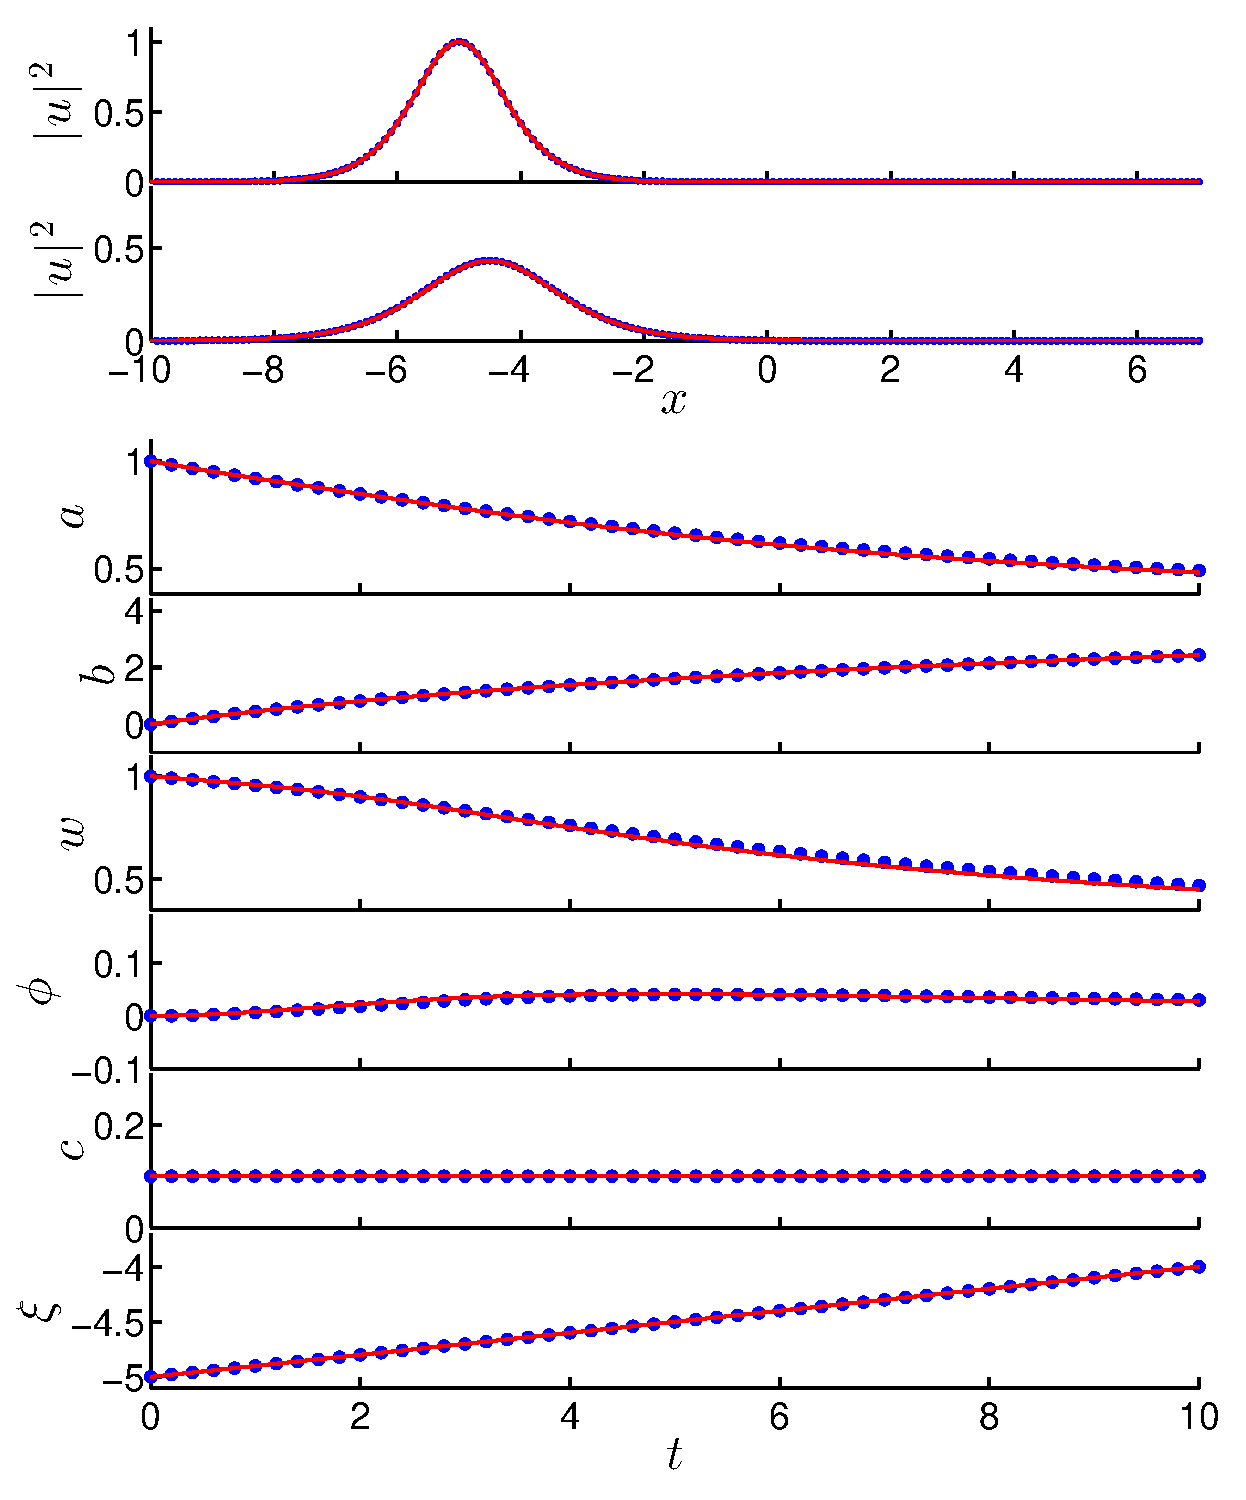
\includegraphics[width=0.8\textwidth]{Fig2_DD_e01N.eps}}
  \rule{35em}{0.5pt}
  \caption[NLS with Density Dependent Loss, $\epsilon = 0.1$]{Evolution of an NLS bright soliton under the presence of nonlinear loss of strength $\epsilon=0.1$.  The NCVA results are obtained from Eq.~(\ref{eq:NVCADD}) (red lines) while the full numerical solution is obtained from Eq.~(\ref{eq:NLSDD}) (blue dots).  Same initial conditions and layout of panels as in previous figures.}
   \label{fig:DDloss01}
\end{figure}
 
%\begin{figure}[htbp]
% \centering
%  \centerline{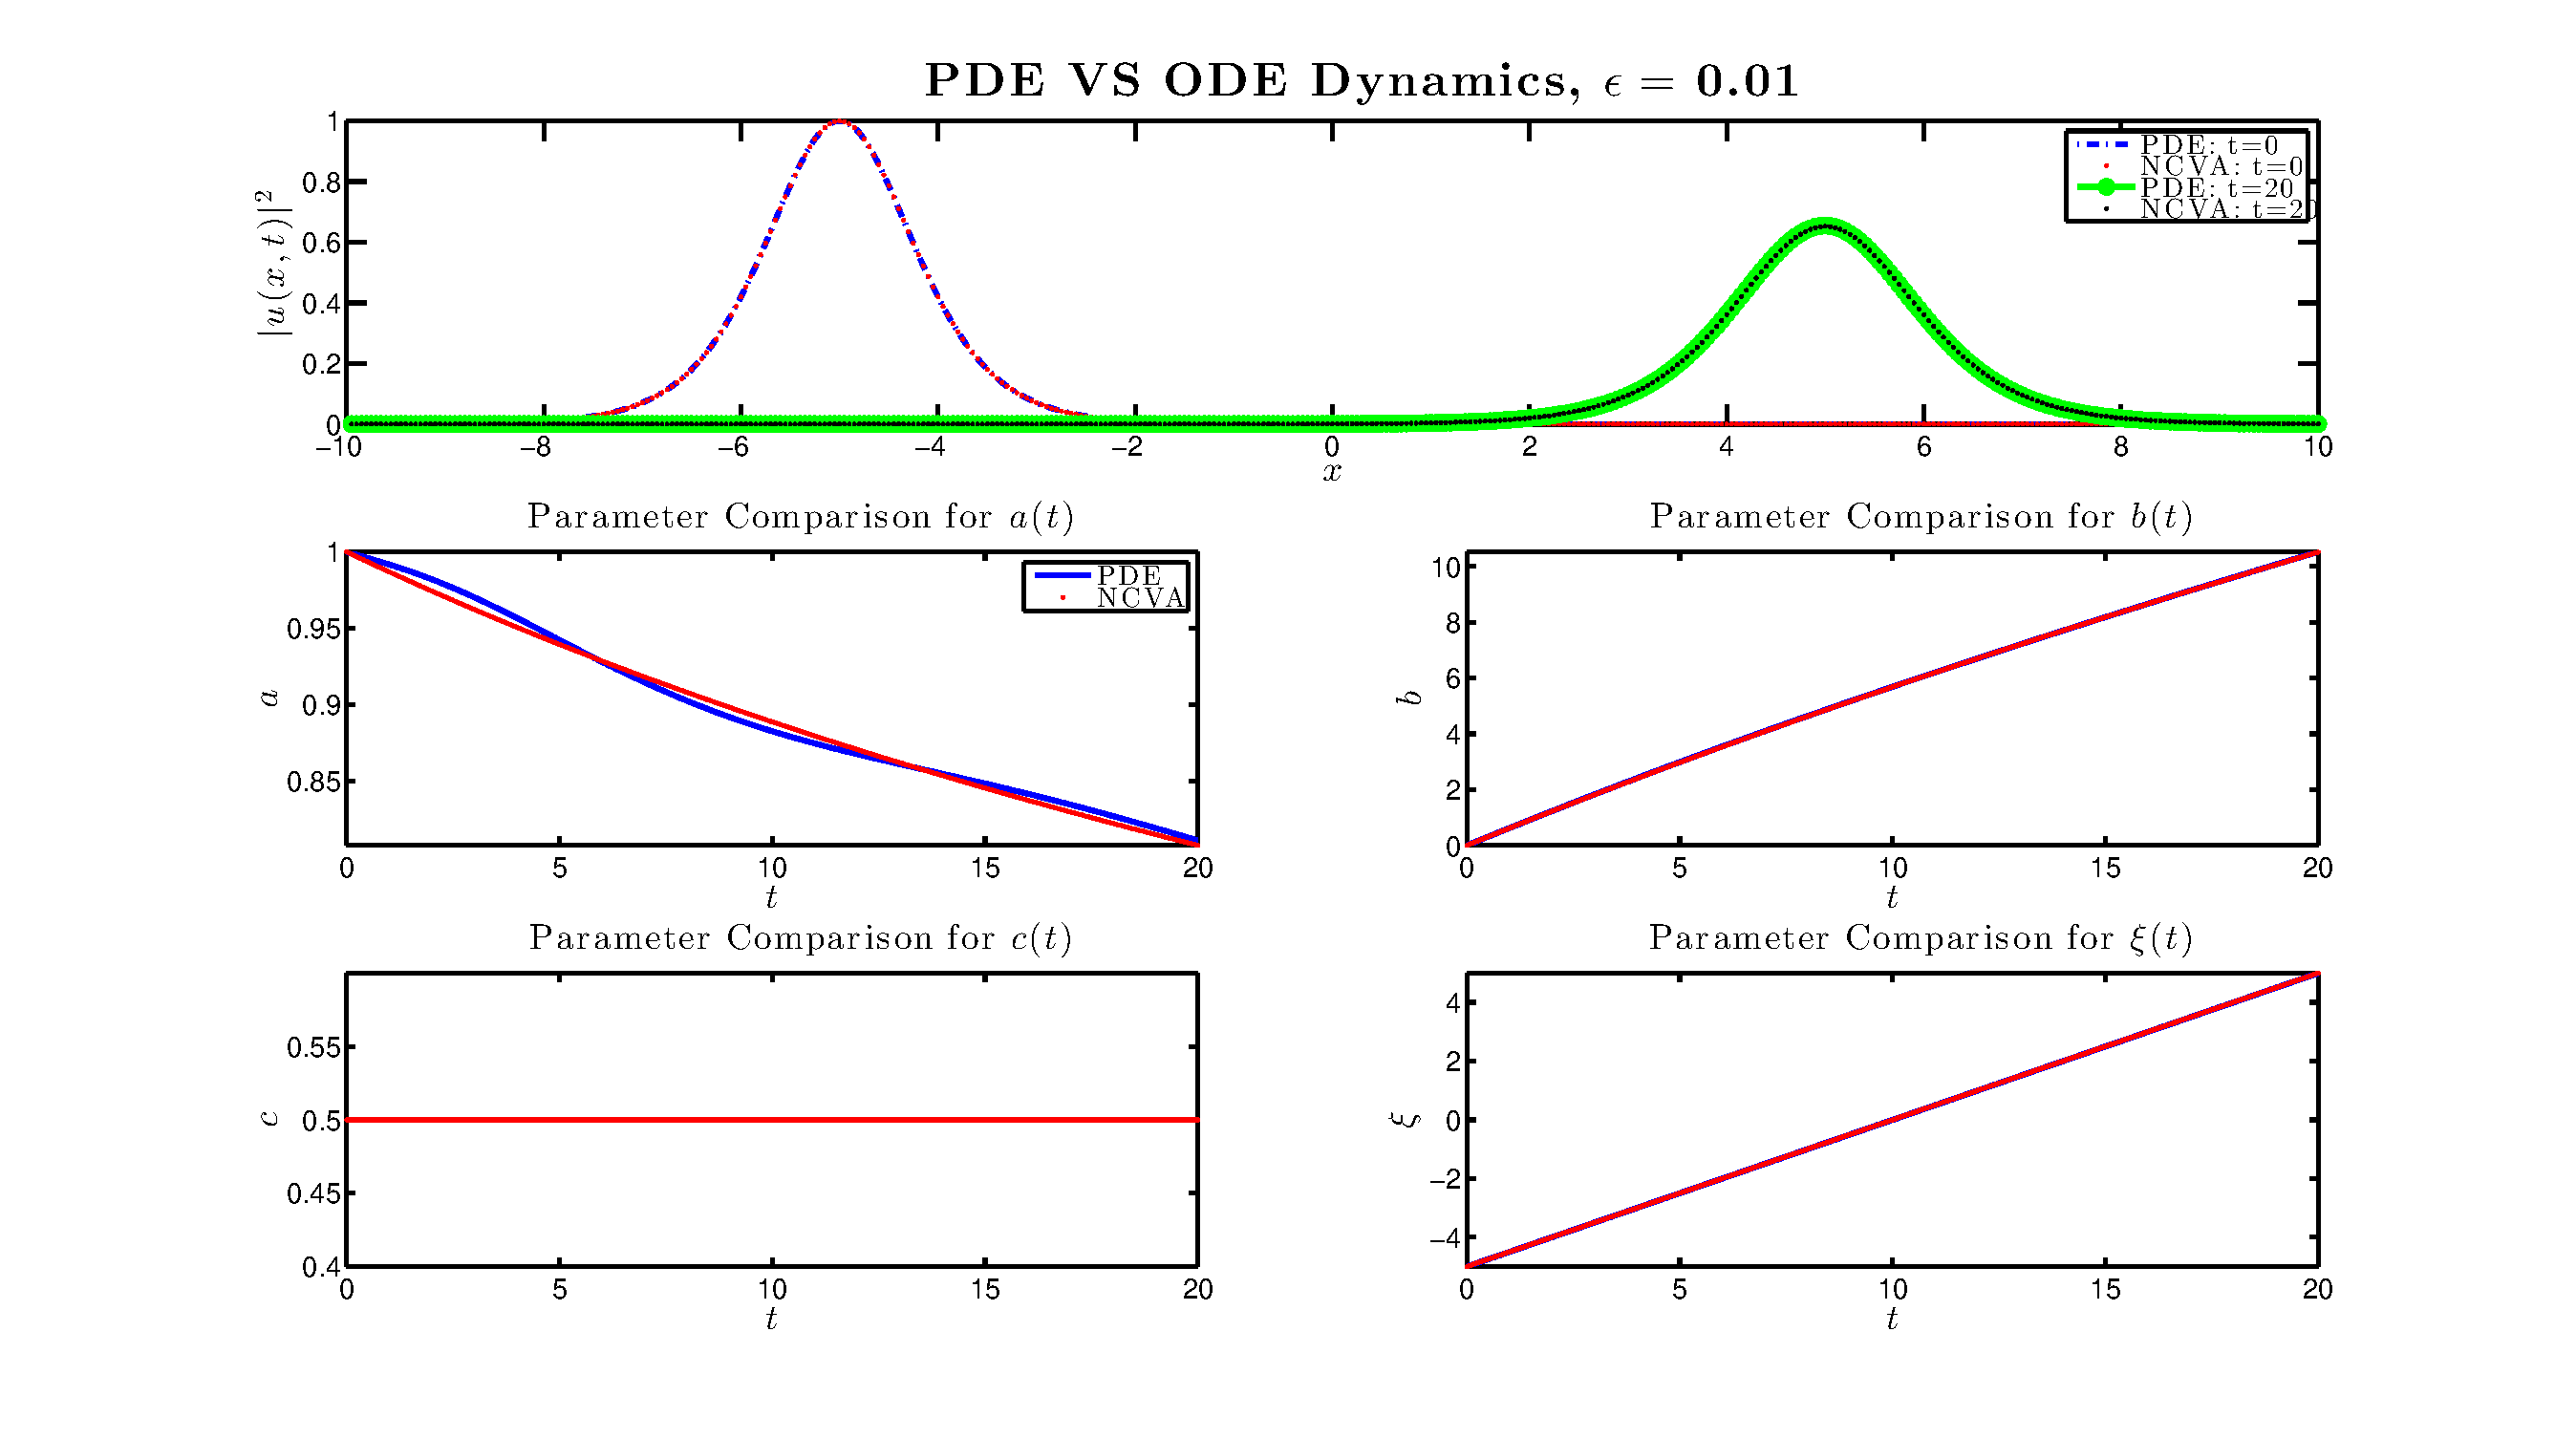
\includegraphics[width=1.2\textwidth, height=\textwidth]{DD001.eps}}
%  \rule{35em}{0.5pt}
%  \caption[NLS with Density Dependent Loss, $\epsilon = 0.01$]{{\bf NLS with Density Dependent Loss:} Comparison of ODE dynamics for the parameters $a$, $b$, $c$, and $\xi$ between forward integration of the PDE and the NCVA for $\epsilon=0.01$.}
%   \label{fig:DDloss001}
%\end{figure}
%
%
%\begin{figure}[htbp]
%  \centering
%  \centerline{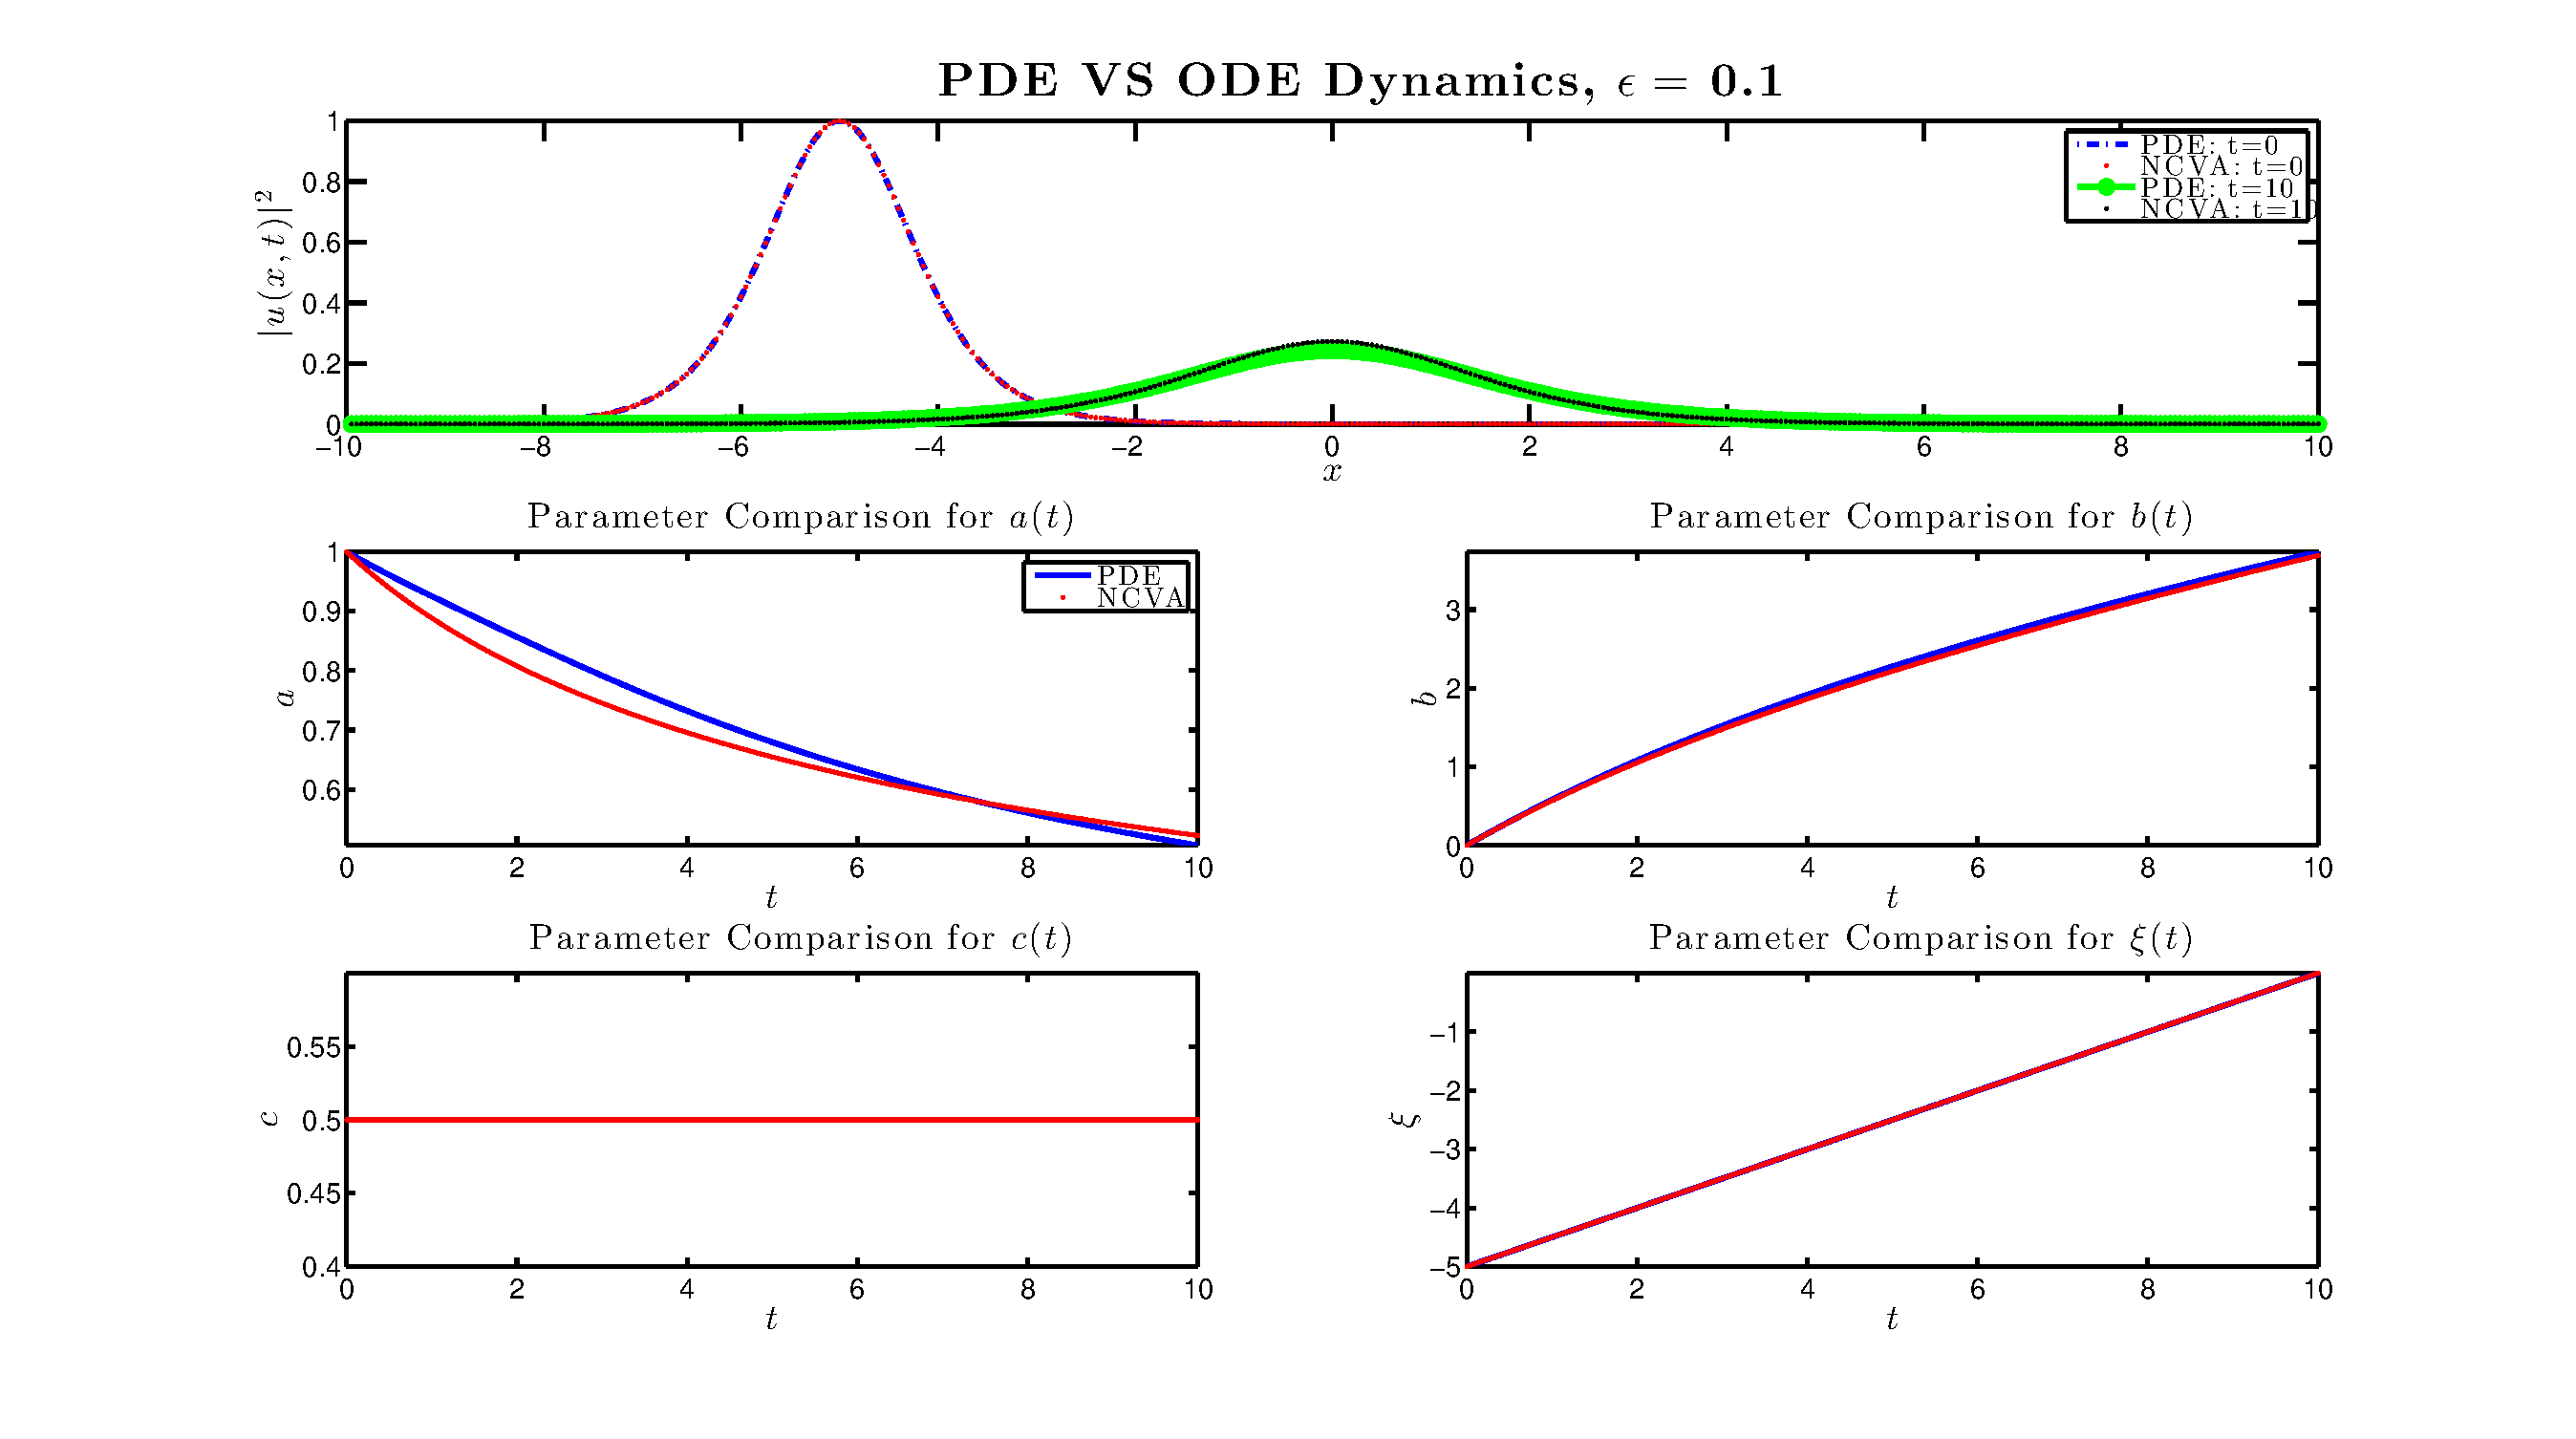
\includegraphics[width=1.2\textwidth, height=\textwidth]{DD01.eps}}
%  \rule{35em}{0.5pt}
%  \caption[NLS with Density Dependent Loss, $\epsilon = 0.1$]{{\bf NLS with Density Dependent Loss:} Comparison of ODE dynamics for the parameters $a$, $b$, $c$, and $\xi$ between forward integration of the PDE and the NCVA for $\epsilon=0.1$.}
%   \label{fig:DDloss01}
%\end{figure}
%
%
%\begin{figure}[htbp]
%\centering
%\begin{subfigure}[t]{0.49\textwidth}
%  		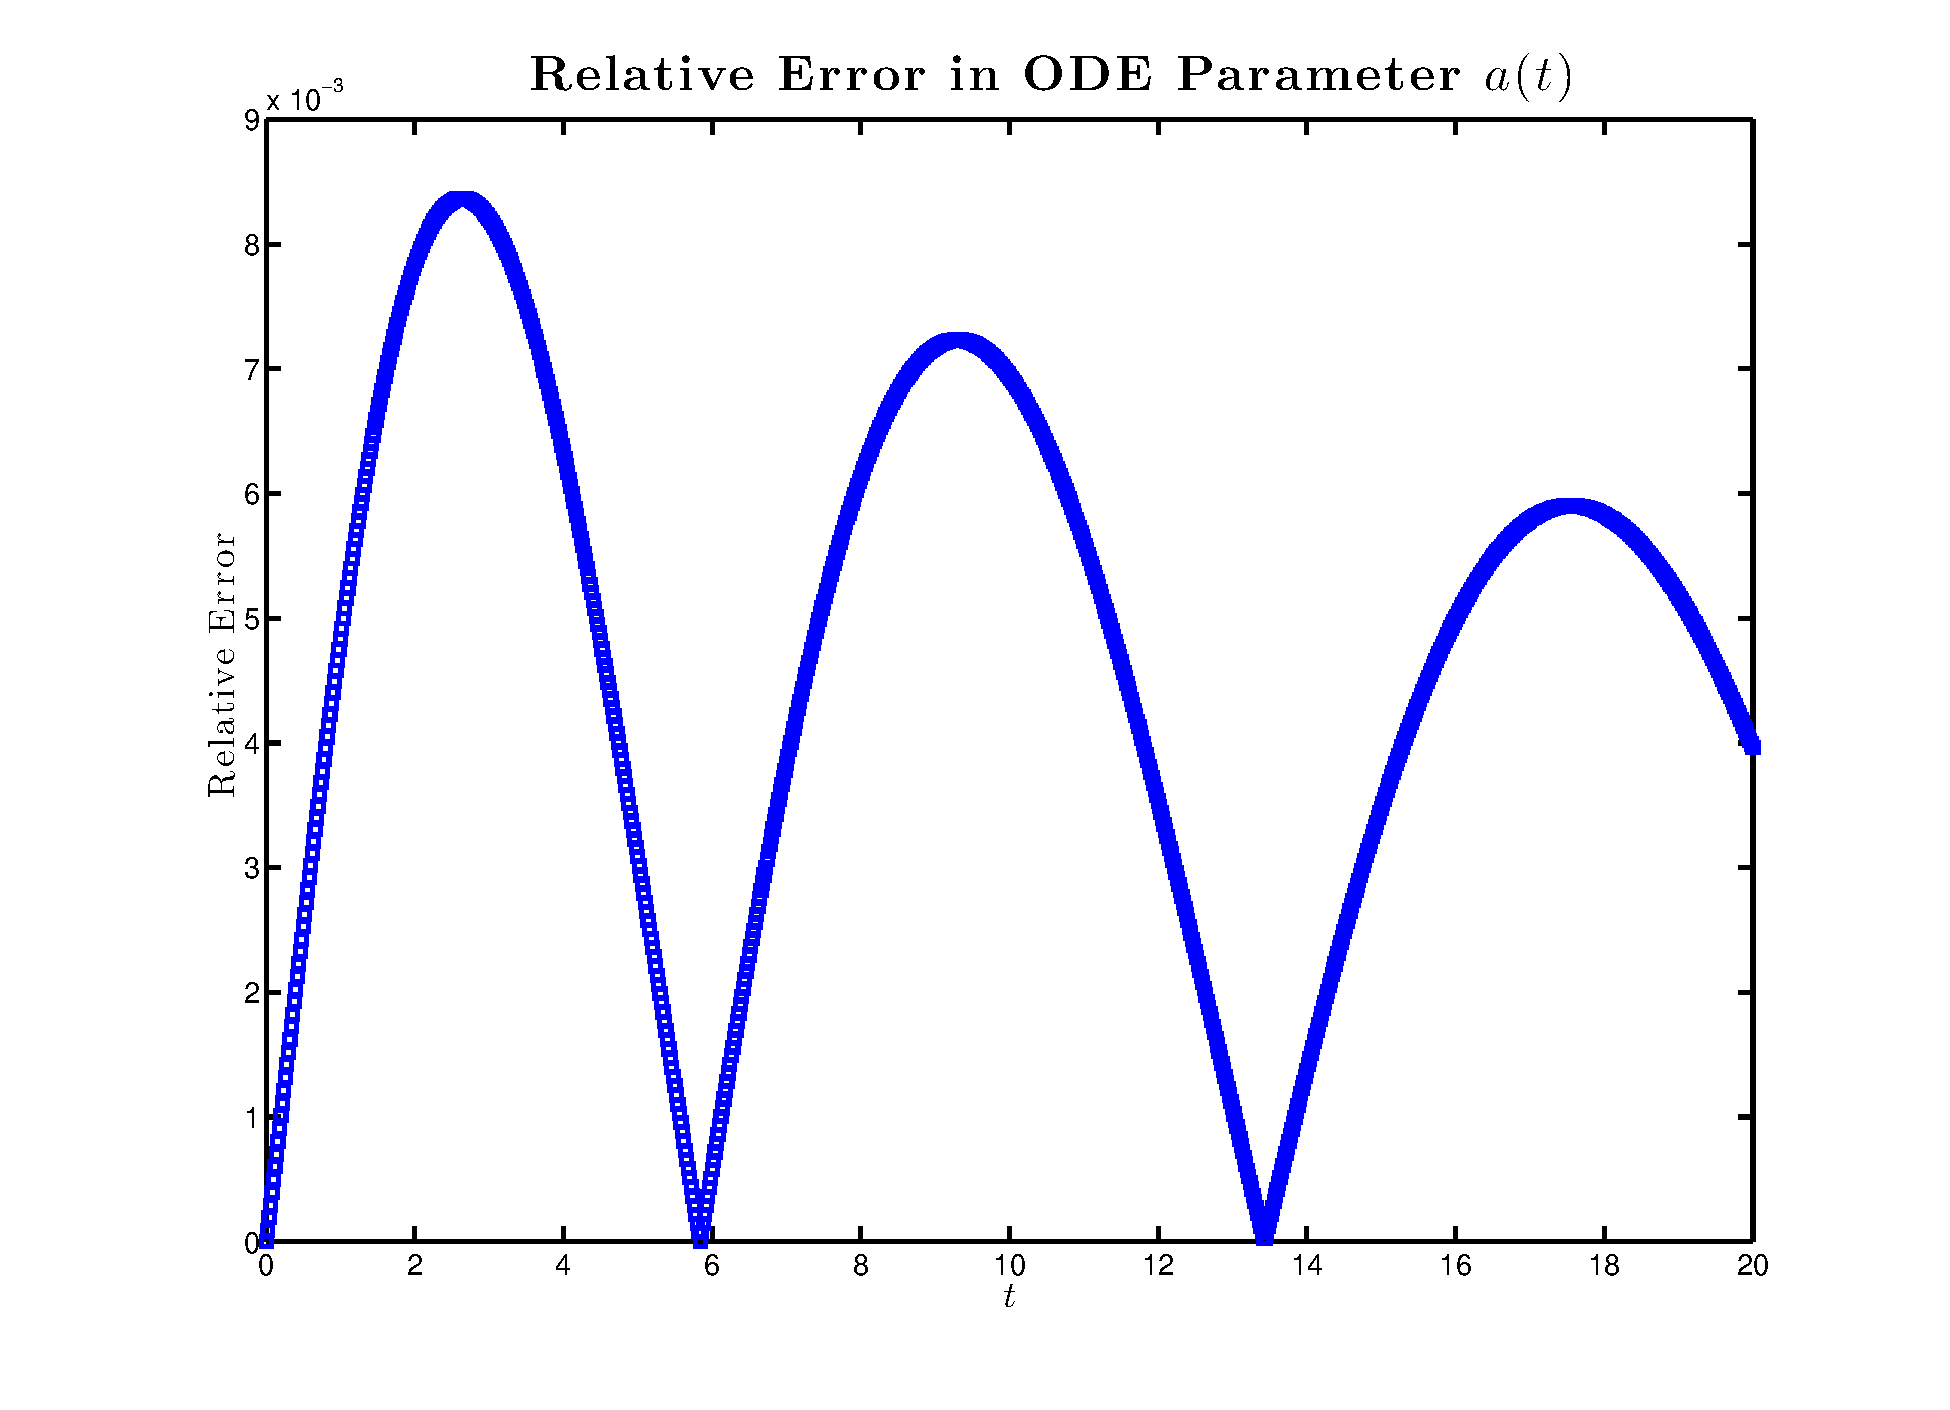
\includegraphics[width=\textwidth, height = \textwidth]{DD001relativeerror.eps}
%	         \caption{Relative error between NCVA and PDE parameter $a(t)$ values for $\epsilon=0.01$.}
%	         \label{fig:DLoss001Err}
%	     \end{subfigure}
%  \begin{subfigure}[t]{0.49\textwidth}
%  		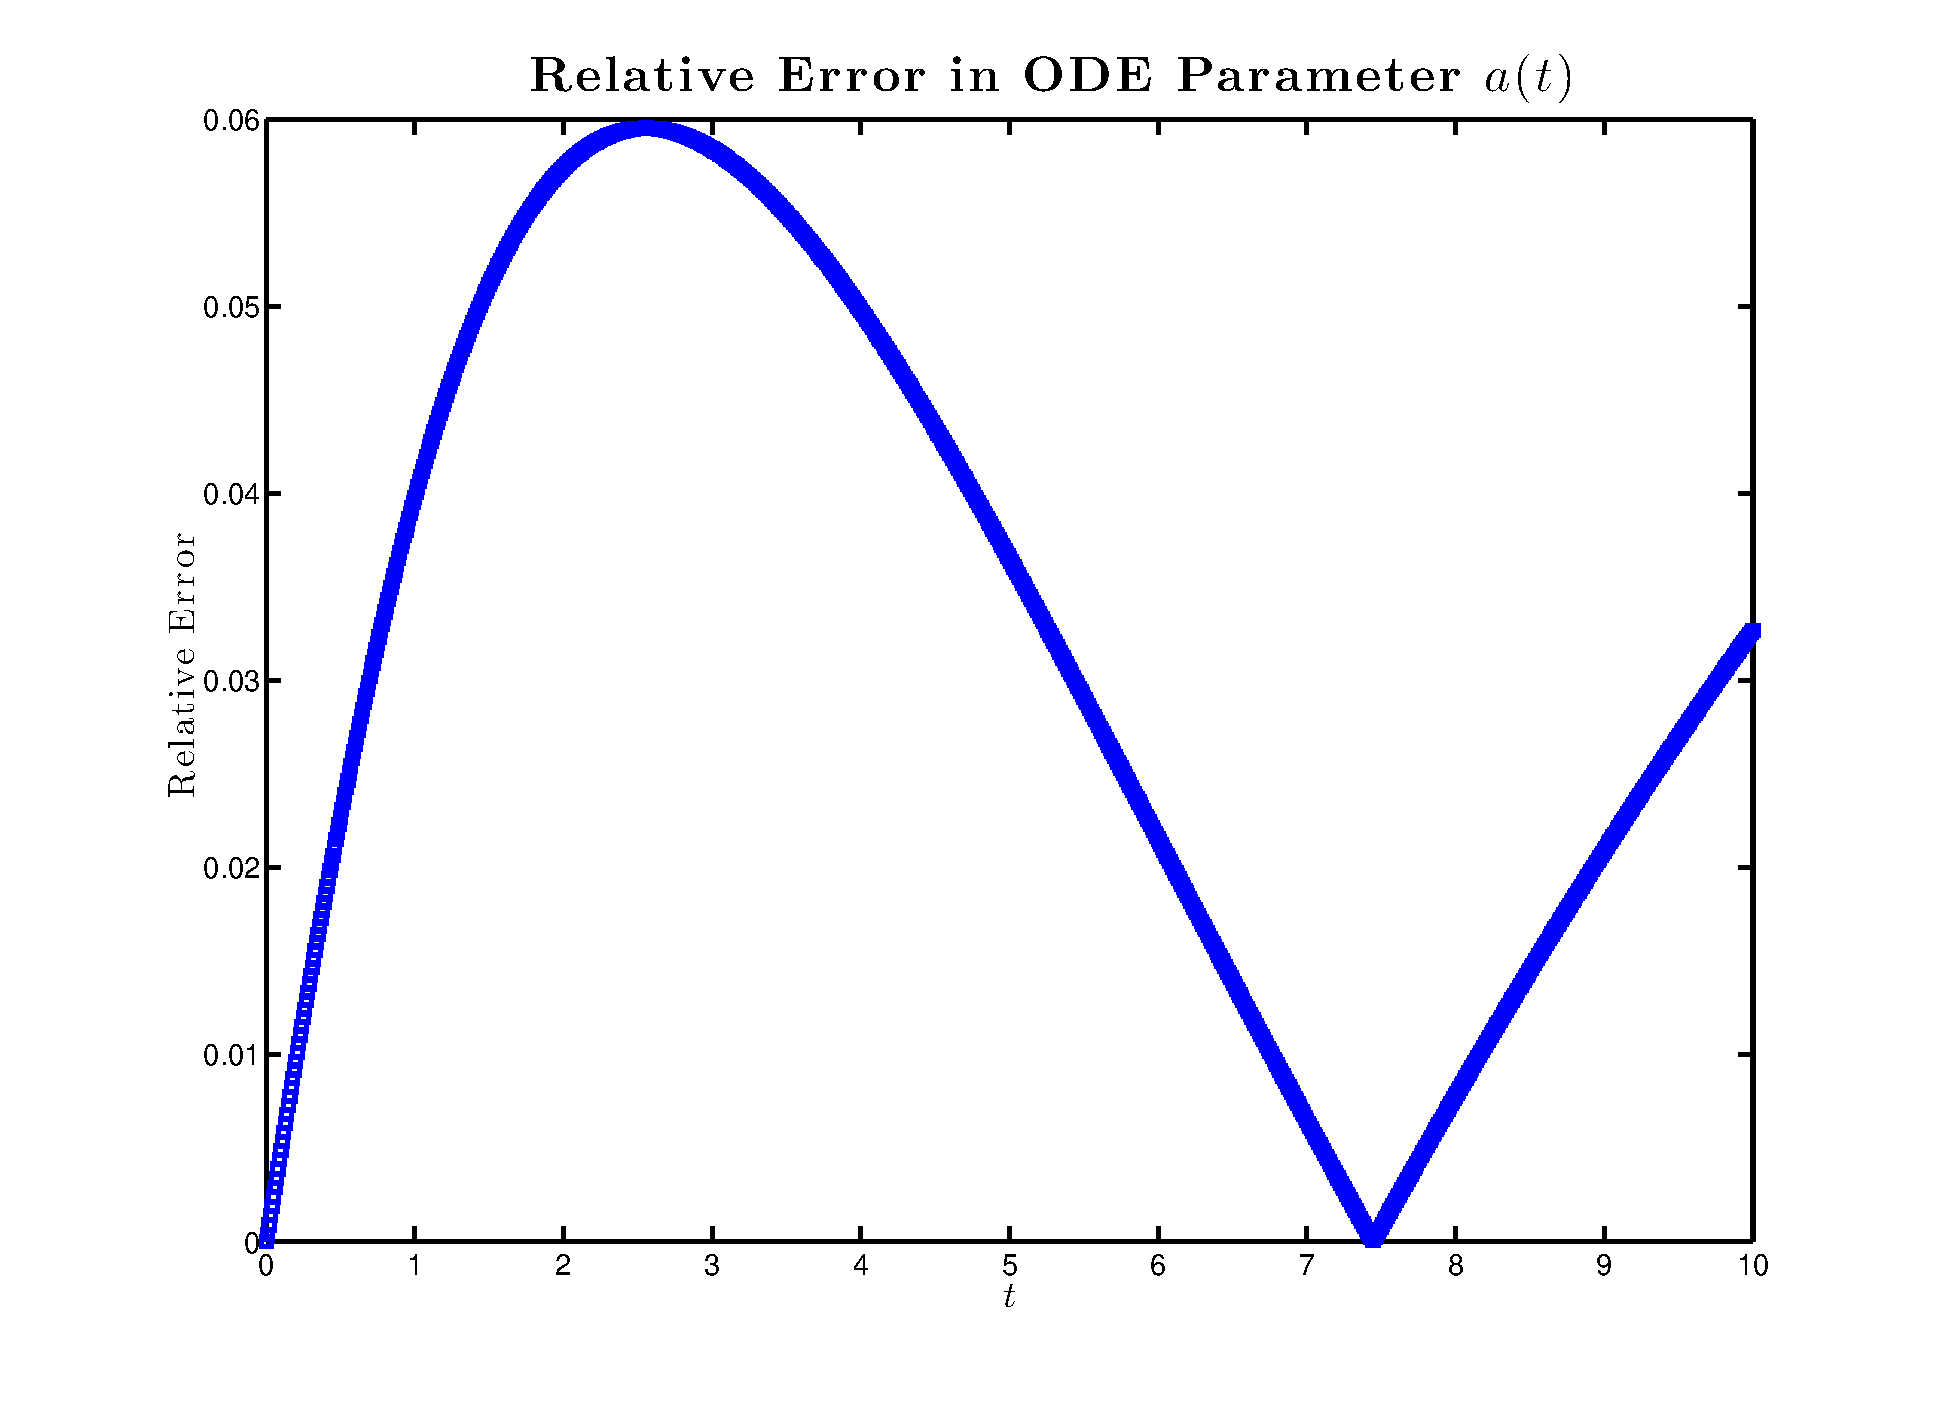
\includegraphics[width= \textwidth, height = \textwidth]{DD01relativeerror.eps}  
%	          \caption{Relative error between NCVA and PDE parameter $a(t)$ values for $\epsilon=0.1$.}
%	         \label{fig:DLoss01Err}
%	    \end{subfigure} 
%  \rule{35em}{0.5pt}
%   \caption[Relative Error in Amplitude for NLS with Density Dependent Loss]{{\bf NLS with Density Dependent Loss:} Amplitude parameter $a(t)$ relative error for (A) $\epsilon=0.01$ and (B) $\epsilon=0.1$.}
%   \label{fig:LLossA}
%\end{figure}

%\begin{figure}[htbp]
%\centering
%\begin{subfigure}[t]{0.49\textwidth}
%  		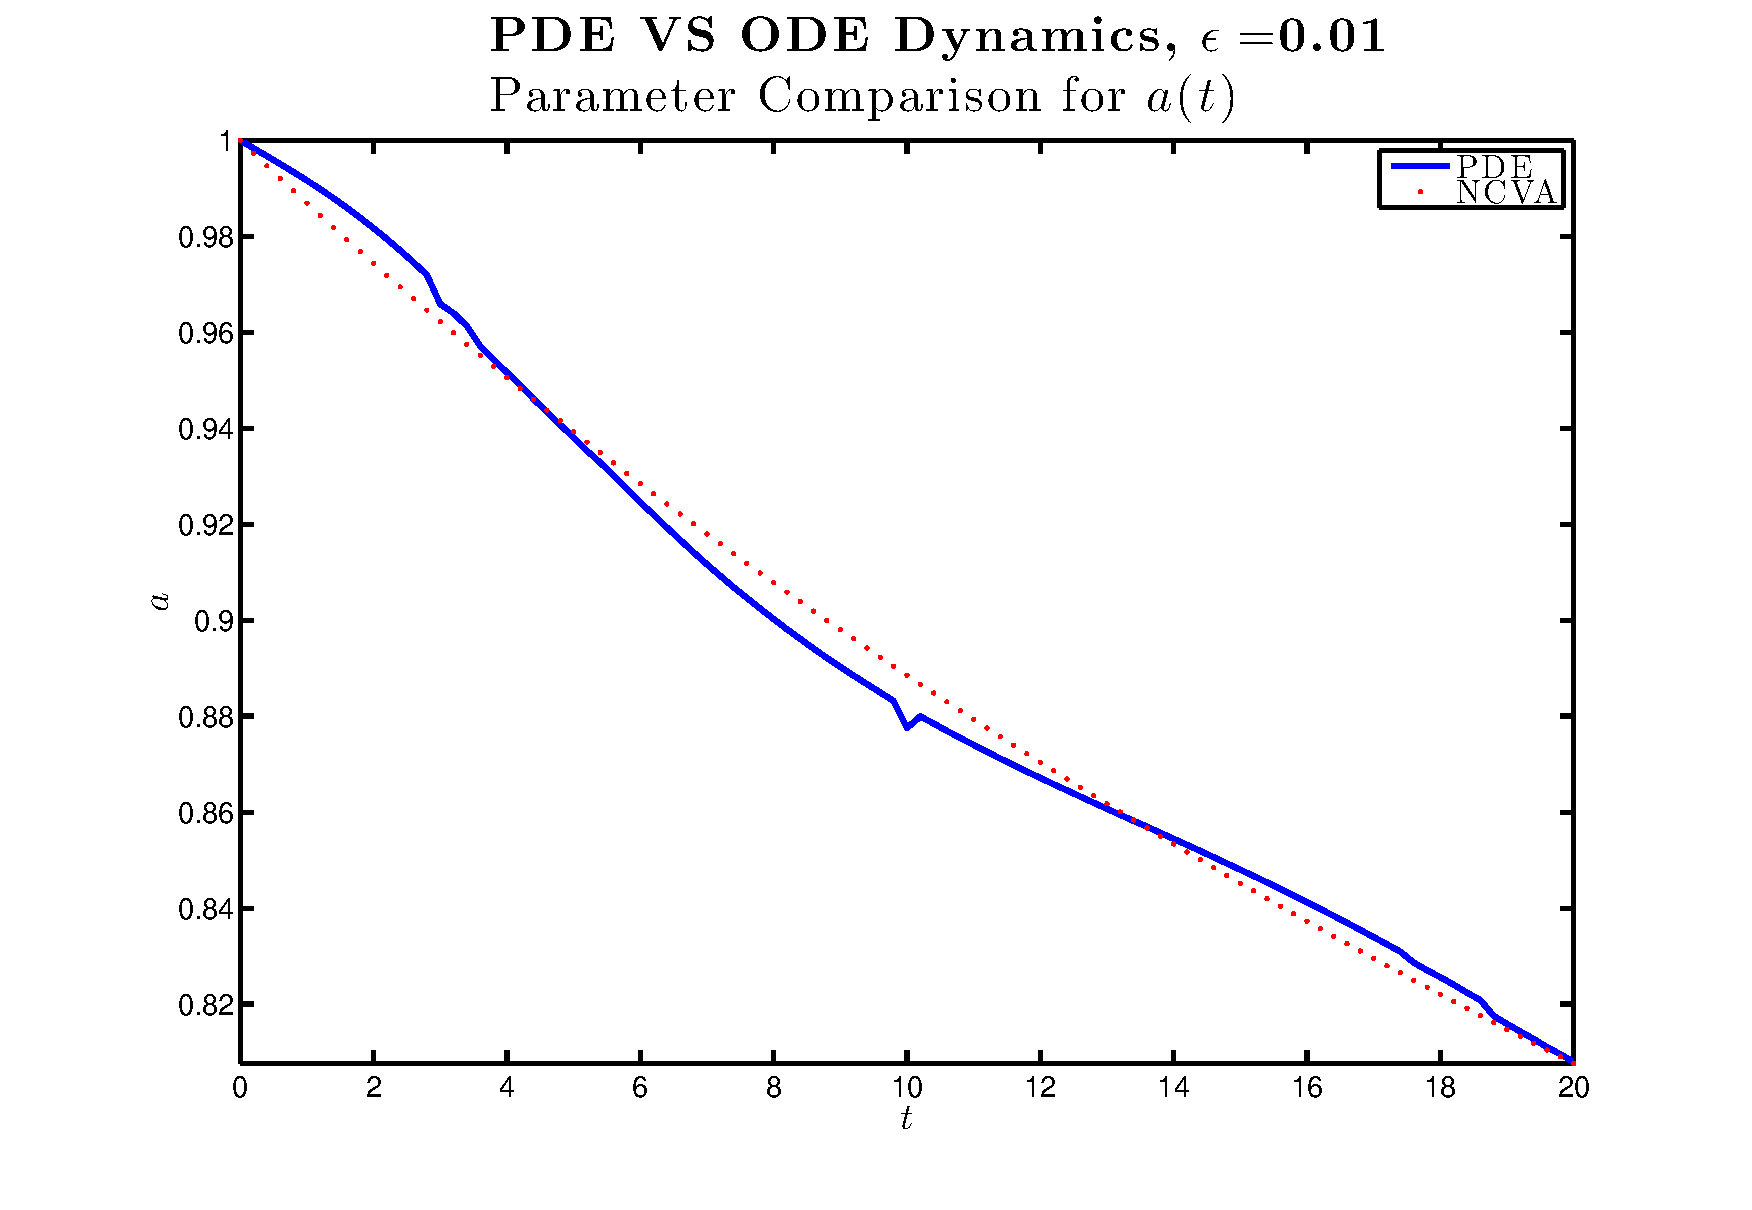
\includegraphics[width=\textwidth, height = \textwidth]{DDE001a.eps}
%	         \caption{Amplitude parameter comparison $a(t)$ between PDE and NCVA solutions.}
%	         \label{fig:DLoss001a}
%	     \end{subfigure}
%  \begin{subfigure}[t]{0.49\textwidth}
%  		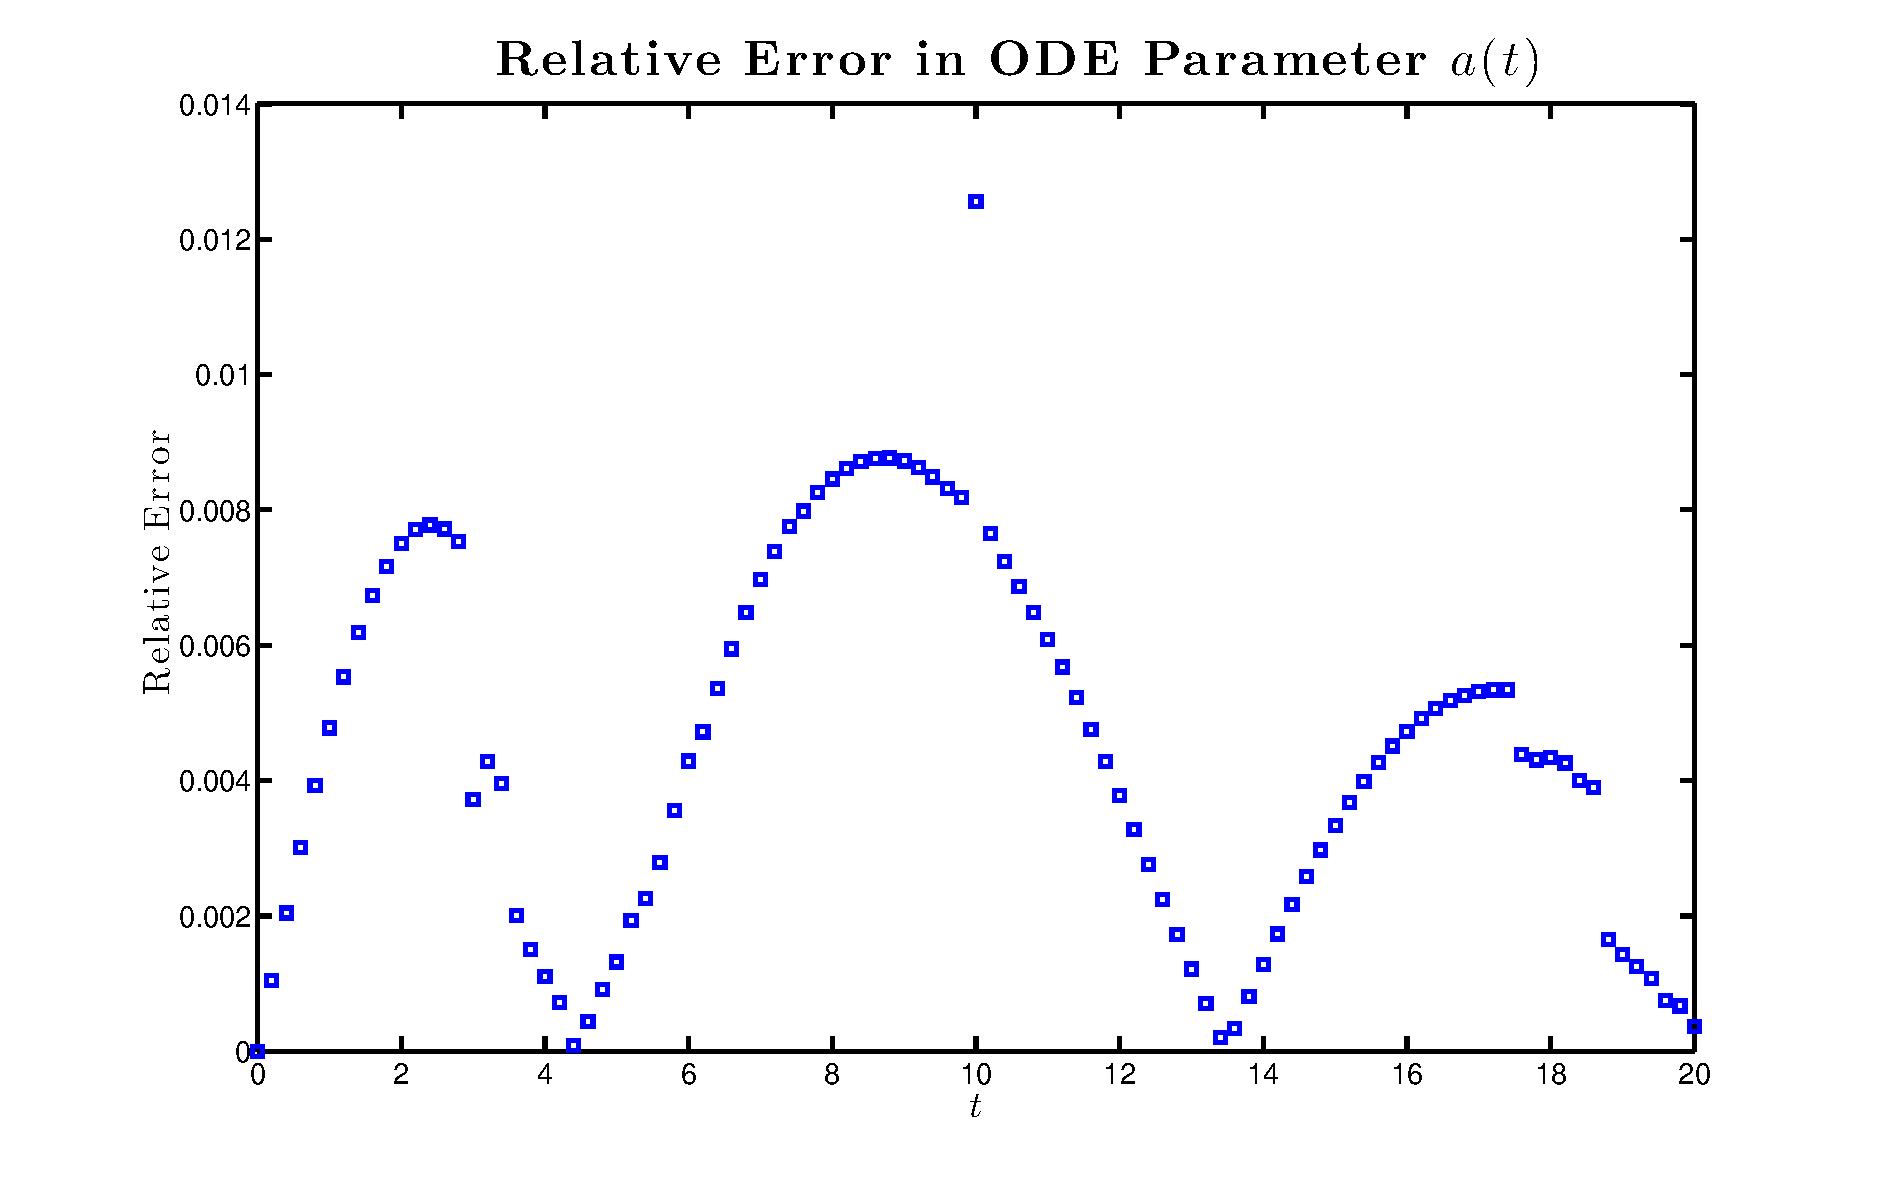
\includegraphics[width= \textwidth, height = \textwidth]{DDE001relativeError.eps}  
%	          \caption{Relative error between NCVA and PDE parameter $a(t)$ values.}
%	         \label{fig:DLoss001Err}
%	    \end{subfigure} 
%  \rule{35em}{0.5pt}
%   \caption[NLS with Density Dependent Loss, $\epsilon = 0.01$ Amplitude Comparison and Relative Error]{{\bf NLS with Density Dependent Loss:} Amplitude parameter $a(t)$ ansatz comparisons and relative error for $\epsilon=0.01$.}
%   \label{fig:DDlossA}
%\end{figure}
%
%
%\begin{figure}[htbp]
%\begin{subfigure}[b]{0.5\textwidth}
%  		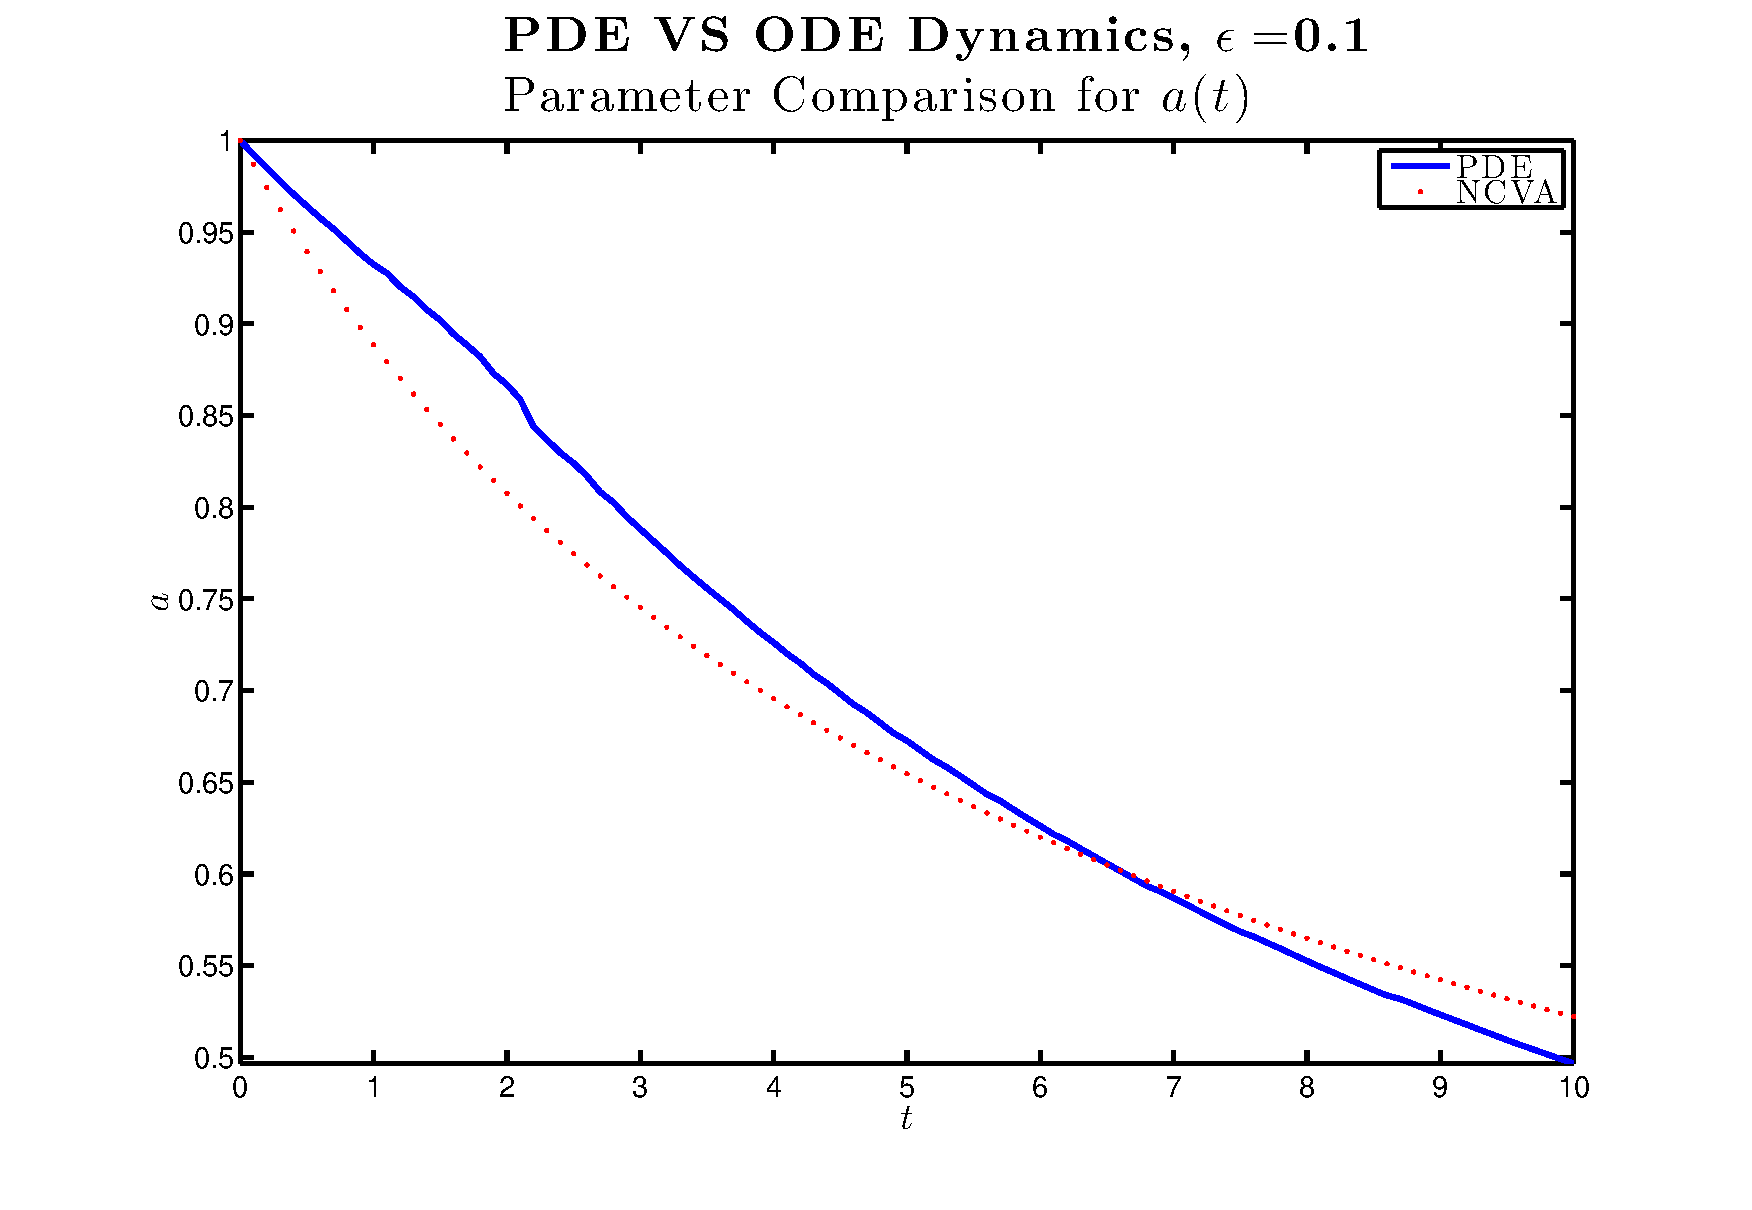
\includegraphics[width=\textwidth, height = \textwidth]{DDE01a.eps}
%	         \caption{Amplitude parameter comparison $a(t)$ between PDE and NCVA solutions.}
%	         \label{fig:DLoss01a}
%	     \end{subfigure}
%  \begin{subfigure}[b]{0.5\textwidth}
%  		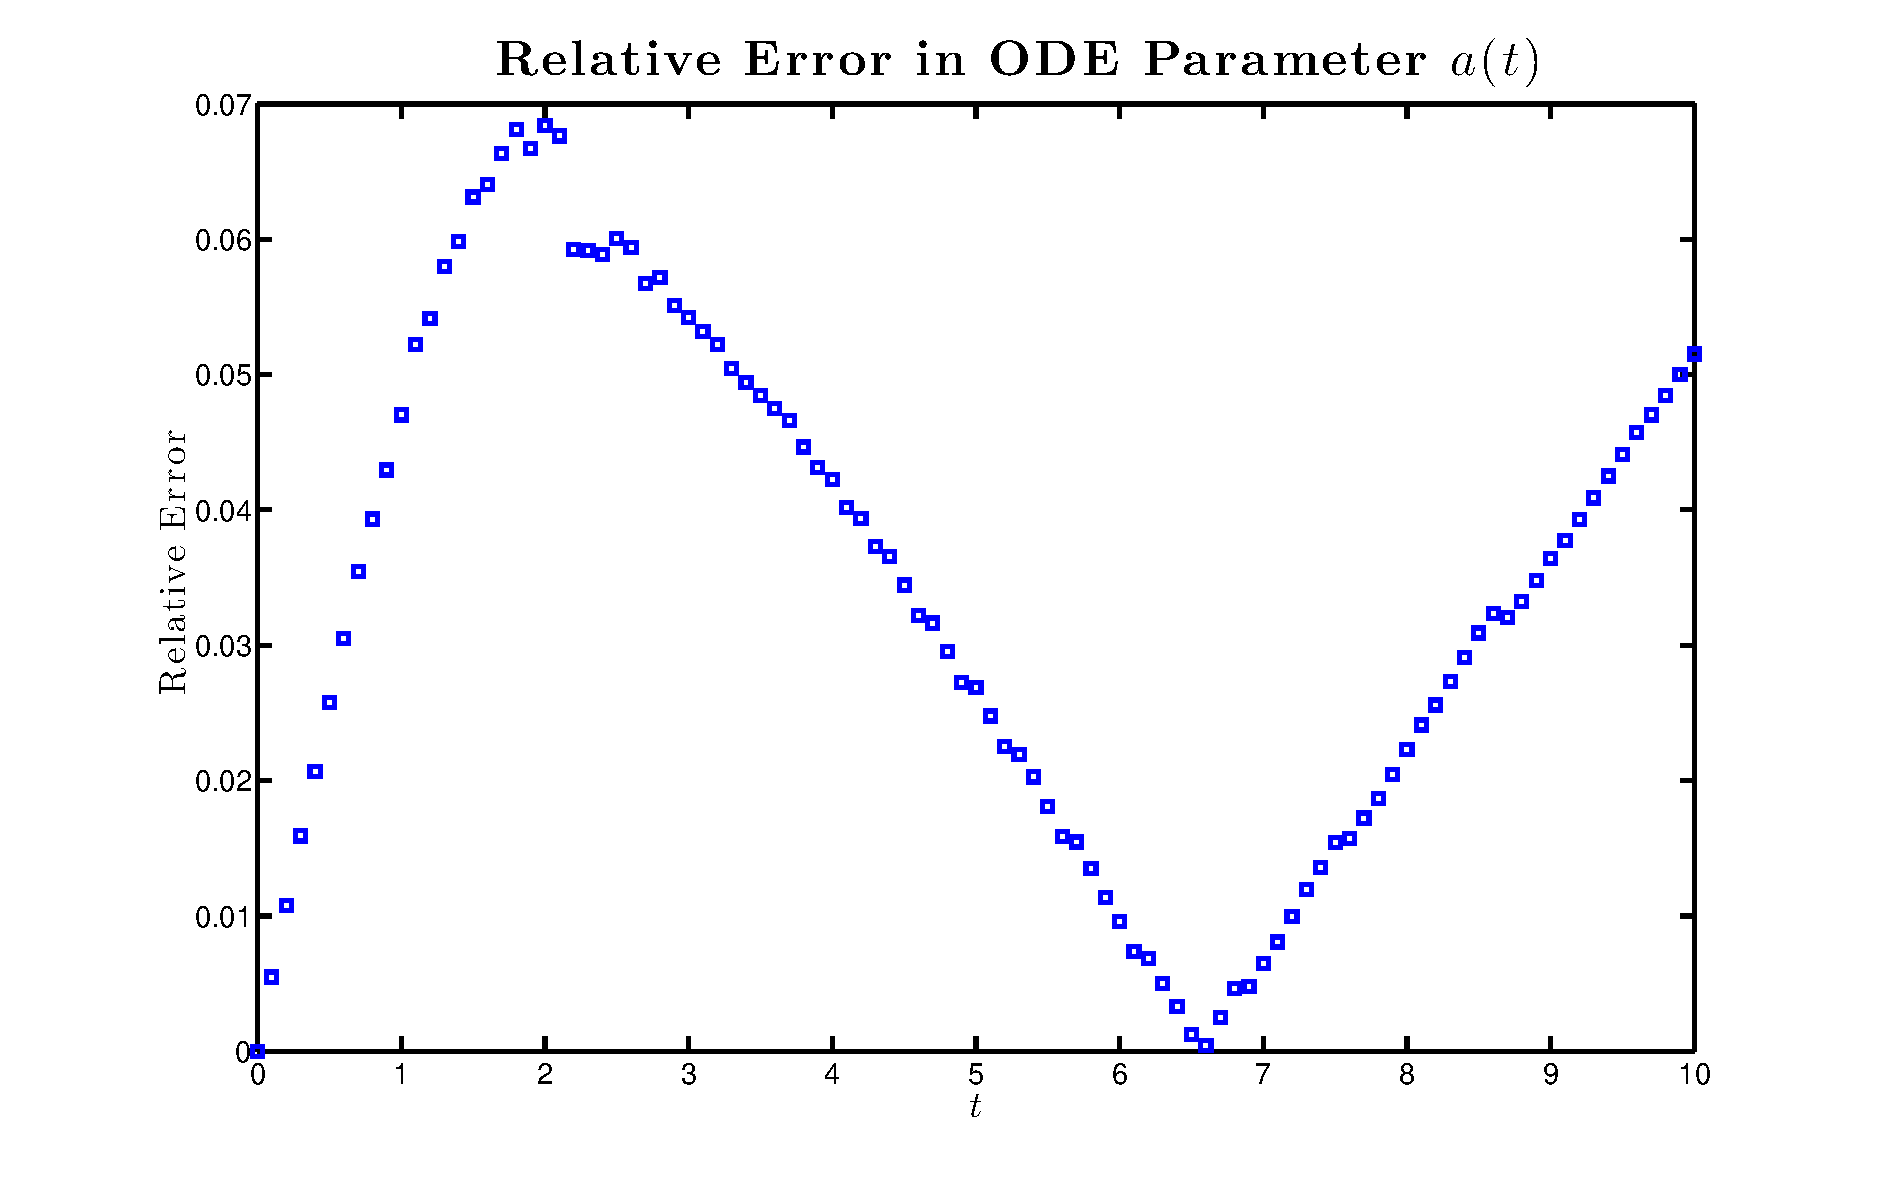
\includegraphics[width= \textwidth, height = \textwidth]{DDE01relativeError.eps}  
%	          \caption{Relative error between NCVA and PDE parameter $a(t)$ values.}
%	         \label{fig:DLoss01Err}
%	    \end{subfigure} 
%  \rule{35em}{0.5pt}
%   \caption[NLS with Density Dependent Loss, $\epsilon = 0.1$ Amplitude Comparison and Relative Error]{{\bf NLS with Density Dependent Loss:} Amplitude parameter $a(t)$ ansatz comparisons and relative error for $\epsilon=0.1$.}
%   \label{fig:DDlossA2}
%\end{figure}

\clearpage

%%%% Section Polariton - NLS with Linear Gain and Density Dependent loss %%%%%%%%%%%
{\setstretch{1.3}
\section[Exciton-Polariton Condensate - The Nonlinear Schr\"{o}dinger Equation with Linear Gain and Density Dependent Loss]{Exciton-Polariton Condensate -  NLS with Linear Gain and Density Dependent Loss}\label{section:EPCond}}

\setstretch{2}
The third dynamical system is based on exciton-polariton condensates.  
In exciton-polariton condensates, the condensing ``entities'' are excitons, namely
bound electron-hole pairs.  These excitons strongly couple with light when confined in quantum wells placed in
high-finesse microcavities, forming exciton-photon mixed quasi-particles known
as polaritons \cite{RMP}.  These condensates exist at finite temperatures, even near room temperature, which means the the polaritons can only exist for a few picoseconds in the cavity before they decay into photons.  The finite lifetime of the polaritons precludes the system from reaching thermal equilibrium, in fact, the system is a genuinely far-from-equilibrium condensate which requires an external pump from a reservoir of excitons to counter the loss of polaritons.

Exciton-polariton condensates offer numerous key features of the superfluid 
character including: the flow without scattering (analog of the flow without friction) \cite{amo1},
the existence of vortices \cite{lagou1}
and their interactions \cite{roumpos,roumpos2},
the collective superfluid dynamics \cite{amo2},
as well as remarkable applications such as spin switches \cite{amo3},
and light emitting diodes \cite{amo4} operating even near room temperatures.

There is a wide variety of different types of models for polaritons to describe the associate pumping and damping mechanisms.  One of these models,
proposed in Refs.~\cite{Keeling2008,kbb,berl_review},
suggests the use of a {\em single} NLS-type equation for the polariton
condensate wavefunction which incorporates a gain-loss mechanism for the decay of polaritons to photons and pumping of excitons from an external reservoir.  Specifically, this model, based on a repulsive ($g=-1$)
NLS equation with linear gain ($i\chi(x) u$)
and density dependent loss ($-i\sigma |u|^2 u$) terms, can be written
in the following non-dimensional form~\cite{ref8,Keeling2008}:
%
\begin{equation}
iu_t + \frac{1}{2} u_{xx} - |u|^2 u - V(x)u =  i\left[\chi(x) - \sigma  |u|^2\right] u, \label{eq:NLSP}
\end{equation}
where $\sigma$ is the strength of the density dependent loss and $\chi$ is considered the localized, spatially dependent gain given by 
\begin{equation}
\chi(x) = \alpha\exp\left(-\frac{x^2}{2 \beta^2}\right),
\label{eq:gainP}
\end{equation}
describing a laser pump of amplitude $\alpha$ and width $\beta$.  The potential $V$ is a general harmonic potential of strength $\Omega$:
\begin{equation}
V(x) = \frac{1}{2} \Omega^2 x^2.
\label{eq:potP}
\end{equation}
For the application of variational approximations, we define the Gaussian ansatz 
\begin{equation}
u_A (x,t; \vec{p}) = a e^{ -\frac{x^2}{2w^2}}  e^{i\left(b x^2 + \phi\right)}, \label{eq:GaussAnsatz}
\end{equation}
where the ansatz parameter $\vec{p}_i = (a_i, w_i, b_i, \phi_i)$ for $i=1$ and 2
represent, respectively, the amplitude, width, chirp, and phase of the ansatz solution.  The departure from a ${\rm sech}$-type ansatz is based on two reasons: (i) the Hamiltonian NLS has a Gaussian-type solution for a low density condensate, and (ii) given a Gaussian-type gain, this ansatz allows us to obtain explicit ODEs through the NCVA.
%
%described by a generic NLS equation with linear gain ($i\chi u$) and density dependent loss ($-i\sigma |u|^2 u$) terms~\cite{Cuevas2011, Keeling2008}:
%\begin{align}
%iu_t + \frac{1}{2} u_{xx} + |u|^2 u =  i(\chi - \sigma  |u|^2) u,
%\end{align}
%where $\chi$ and $\sigma$ are, respectively, the gain and loss coefficients. 
%The Lagrangian corresponding to the conservative portion ($\chi = 0$ and $\sigma=0$) is given by:
%\begin{align}
%L = \frac{i}{2} \Bigg( u \frac{\partial u^*}{\partial t} -u^* \frac{\partial u}{\partial t} \Bigg) + \frac{1}{2} \Bigg| \frac{\partial u}{\partial x} \Bigg|^2  - \frac{1}{2} | u|^4.
%\end{align}
%The proposed ansatz is
%\begin{align}
%u(x,t) = a \mathrm{sech}(a(x-\xi))e^{i(c(x-\xi)+b)}
%\end{align}
%with function parameters $a$, $b$, $c$, and $\xi$. 

%\subsection{Perturbed Variational Approximation}
%In the perturbed and Kantorovitch variational approximation methods, the non-conservative terms are 
%\begin{align}
%\mathcal{P} = \chi \mathcal{Q}_{\mathrm{gain}} + \sigma \mathcal{Q}_{\mathrm{loss}} = i(\chi - \sigma  |u|^2) u,
%\end{align}
%such that $\mathcal{Q}_{\mathrm{gain}} = i u$ and $\mathcal{Q}_{\mathrm{loss}} = - i |u|^2 u$
%%According to Cerda's~\cite{Cerda} method the non-conservative terms are described as
%%\begin{align}
%%Q = i(\chi - \sigma  |u|^2) u,
%%\end{align}
%and the two solutions are equivalent.  From the modified Kantorovitch method and the perturbed variational approximation it is straightforward to obtain a system of four coupled ODEs for the exciton-polariton condensate:
%%\begin{align} \begin{cases}
%%2 \dot{b} - a^2 - 2c\dot{\xi} + c^2 = 0, \\
%%-2\dot{a} = -4\chi a +  \frac{8}{3} \sigma a^3, \\
%%-2\dot{\xi} a + 2ac = 0, \\
%%2 \dot{a} c + 2 a \dot{c} = 4\chi a c -\frac{8}{3} \sigma a^3 c. 
%%\end{cases} \end{align} 
%%The four equations are solved simultaneously to find the following system of ODEs for the exciton-polariton condensate: 
% \begin{equation}
% \begin{cases}
%  \dot{a} = \frac{\sqrt{2}}{8} \sigma a^3 -\frac{3\sqrt{2}}{4} \frac{\sigma a^3 w^2}{w^2 + 2\beta^2 } + \frac{3\sqrt{2}}{2} \frac{\alpha \beta a w^2}{\left( w^2 + 2 \beta^2 \right)^{3/2}} -\frac{3\sqrt{2}}{2} \frac{\sigma \beta^2 a^3 }{w^2 + 2\beta^2} + \frac{2\sqrt{2} \alpha \beta^3 a}{\left( w^2 + 2\beta^2\right)^{3/2}} - ab , \\
%\dot{b}  = \frac{\sqrt{2}}{4} \frac{a^2}{w^2} + \frac{1}{2 w^4} - \frac{1}{2} \Omega^2 - 2b^2, \\
%\dot{w} = -\frac{5\sqrt{2}}{4} \sigma a^2 w + \frac{3\sqrt{2}}{2} \frac{\sigma a^2 w^3}{w^2 + 2\beta^2} - \frac{\sqrt{2} \alpha \beta w^3}{\left( w^2 + 2\beta^2 \right)^{3/2}} +\frac{3\sqrt{2} \sigma \beta^2 a^2 w }{w^2 + 2\beta^2} + 2 w b, \\
%\dot{\phi} = -\frac{5\sqrt{2}}{8} a^2 -\frac{1}{2w^2} .
%\end{cases}
% \label{eq:PVAP}
% \end{equation}
%%\begin{align}\begin{cases}
%%\dot{a} = 2\chi a -\frac{4}{3} \sigma a^3, \\
%%\dot{b} = \frac{1}{2} a^2 + \frac{1}{2} c^2, \\
%%\dot{c} = 0,\\
%%\dot{\xi} = c.
%%\end{cases} \label{eq:PVAP}\end{align}

\subsection{Non-conservative Variational Approximation}
In the NCVA, we use two ans\"atze $\bar{u}_1= u_A(x,t; \vec{p_1})$ and $\bar{u}_2=u_A(x,t; \vec{p_2})$ as defined by the Gaussian profile of Eq.~(\ref{eq:GaussAnsatz}).  The selection of a Gaussian profile is to characterize the breathing motion of a ground state inside the trap, rather than to characterize the translational dynamics of the wavefunction.  In order to find translational modes, we would require a different ansatz with an added degree of freedom corresponding to a center position parameter of the wavefunction.

According to the NCVA method, the Lagrangian is $\bar{\mathcal{L}} = \bar{\mathcal{L}}_1 - \bar{\mathcal{L}}_2 +\bar{\mathcal{R}}$, where the conservative terms have the Lagrangian densities for $i= 1,$ 2 given by 
\begin{eqnarray}
\bar{\mathcal{L}_i} &= \frac{i}{2} \left(\bar{u}_i \bar{u}_{i,t}^* - 
\bar{u}_i^* \bar{u}_{i,t}\right) + \frac{1}{2} |\bar{u}_{i,x}|^2 + \frac{1}{2}|\bar{u}_i|^4 + V(x) |\bar{u}_i|^2,
%\bar{\mathcal{L}_1} &= \frac{i}{2} \left(\bar{u}_1 \bar{u}_{1,t}^* - 
%\bar{u}_1^* \bar{u}_{1,t}\right) + \frac{1}{2} |\bar{u}_{1,x}|^2 + \frac{1}{2}|\bar{u}_1|^4 + V(x) |\bar{u}_1|^2,  \\
%\bar{\mathcal{L}}_2 &= \frac{i}{2} \left(\bar{u}_2 \bar{u}_{2,t}^* - \bar{u}_2^* \bar{u}_{2,t}\right) + \frac{1}{2} |\bar{u}_{2,x}|^2 + \frac{1}{2}|
%\bar{u}_2|^4 + V(x) |\bar{u}_2|^2, %\quad\\[1.0ex]
\end{eqnarray}
and $\bar{\mathcal{R}}$ has the same type of density dependent loss [see Section~\ref{section:DD}] and a linear gain (equivalent to the negative of linear loss)  [see Section~\ref{section:NCVALL}] shown in the previous examples.  The non-conservative terms are defined as follows:
\begin{eqnarray}
\bar{\mathcal{R} }&=& \, \bar{\mathcal{P}} u_-^*+ \bar{\mathcal{P}}^*u_-,  \\
&=& -i \chi(x) \left( \bar{u}_2 \bar{u}_1^* -  \bar{u}_1  \bar{u}_2^* \right) \\ \nonumber
&& + i\sigma [ | \bar{u}_1|^2 \left(  \bar{u}_2  \bar{u}_1^* -  \bar{u}_2^*  
\bar{u}_1 \right) +  | \bar{u}_2|^2 \left(  \bar{u}_2  \bar{u}_1^*  - \bar{u}_2^*  \bar{u}_1 \right) +  \bar{u}_2  \bar{u}_2  \bar{u}_1^*  \bar{u}_1^* -  \bar{u}_1  
\bar{u}_1  \bar{u}_2^*  \bar{u}_2^2  ]. 
\end{eqnarray}
%
%In the non-conservative variational approximation $u_1$ and $u_2$ ansatz are defined as
%\begin{align}
%u_1 &= a_1 \mathrm{sech}(a_1(x-\xi_1))e^{i(c_1 (x-\xi_1)+b_1)}, \\
%u_2 &= a_2 \mathrm{sech}(a_2(x-\xi_2))e^{i(c_2 (x-\xi_2)+b_2)}.
%\end{align}
%According to the non-conservative variational method the Lagrangian is $\mathscr{L} = L_1 - L_2 + R$ where 
%\begin{align}
%L_1 =& \frac{i}{2} \Big(u_1 u_{1,t}^* - u_1^* u_{1,t}\Big) + \frac{1}{2} |u_{1,x}|^2 - \frac{1}{2}|u_1|^4, \\
%L_2 =& \frac{i}{2} \Big(u_2 u_{2,t}^* - u_2^* u_{2,t}\Big) + \frac{1}{2} |u_{2,x}|^2 - \frac{1}{2}|u_2|^4, \\
%Q =&  -i\chi u_+ u_-^* + i\sigma  u_+ u_+^* u_+u_-^* \nonumber \\
%=&  -i \chi \frac{(u_1 + u_2)}{2}(u_1 - u_2)^*  +  i \sigma  \frac{(u_1 + u_2)}{2}\frac{(u_1^* + u_2^*)}{2}\frac{(u_1 + u_2)}{2}(u_1 - u_2)^* \nonumber \\
%=& -\frac{i}{2} \chi (u_1u_1^* - u_2 u_2^* + u_2u_1^* - u_1 u_2^*) \nonumber \\
%&+ \frac{i}{8} \sigma (|u_1|^4 - |u_2|^4 + |u_1|^2(2u_2u_1^*) -  |u_2|^2(2u_1 u_2^*)  + u_2u_2 u_1^*u_1^* - u_1u_1u_2^*u_2^*) \\
%\begin{align}
%R =& \, Q + Q^*, \nonumber \\
%=& -i \chi (u_2u_1^* - u_1 u_2^* ) + i\sigma ( u_+ u_+^* u_+u_-^* -  u_+ u_+^* u_-u_+^*).
%\end{align}
%The modified Euler-Lagrange equations:
%\begin{align}
%\frac{\partial L}{\partial p} - \frac{d}{dt} \Bigg( \frac{\partial L }{\partial\dot{p}}\Bigg) + \int \Big[ \frac{\partial R}{\partial p_-} \Big]_{\mathrm{PL}} dx = 0. 
%\end{align}
%The total Lagrangian:
%\begin{align} \bar{L} =& 2\dot{b}_1a_1 - \frac{1}{3}a_1^3 + c_1^2 a_1 - 2c_1 \dot{\xi}_1a_1 - 2\dot{b}_2 a_2 + \frac{1}{3}a_2^3 - c_2^2 a_2 + 2c_2 \dot{\xi}_2 a_2  \nonumber  \\ 
%&- i \chi \int \Big[ \frac{\partial}{\partial p_-} \Big(u_2u_1^* - u_1u_2^*)\Big]_{\mathrm{PL}} dx \nonumber \\ 
%&+ \frac{i}{4} \sigma \int \Big[ \frac{\partial}{\partial p_-} \Big(|u_1|^2( u_2u_1^* - u_2^* u_1) +  |u_2|^2( u_2u_1^* - u_2^* u_1)  + u_2u_2 u_1^*u_1^* - u_1u_1u_2^*u_2^*\Big) \Big]_{\mathrm{PL}} dx . \end{align}
For all the parameters we made the substitutions of $\pm$ coordinates into the expression for the total Lagrangian and from the $
\bar{\mathcal{L}}_1$ and $\bar{\mathcal{L}}_2$ parts we recover the conservative Euler-Lagrange equations for a Gaussian ans\"{a}tz with 
four-parameters.
From the non-conservative term $\bar{\mathcal{R}}$, we expand in the $\pm$ coordinate systems and find the integrals, which are combinations of the 
integrals for linear gain and density dependent loss [see Sections~\ref{section:NCVALL} and~\ref{section:DD}]:
\begin{eqnarray}
\int_{-\infty}^{\infty} \left[ \frac{\partial  \bar{\mathcal{R}}}{\partial a_-} \right]_{\rm PL} dx &=& 0,  \nonumber  \\
\int_{-\infty}^{\infty} \left[ \frac{\partial  \bar{\mathcal{R}}}{\partial b_-} \right]_{\rm PL} dx &=& -\frac{\sqrt{2\pi}}{4}  \sigma a^4 w^3 + \frac{2\sqrt{2\pi} \alpha \beta^3 a^2 w^3}{\left( w^2 + 2\beta^2 \right)^{3/2}} , \nonumber \\
\int_{-\infty}^{\infty} \left[ \frac{\partial  \bar{\mathcal{R}}}{\partial w_-} \right]_{\rm PL} dx &=& 0, \nonumber \\
\int_{-\infty}^{\infty} \left[ \frac{\partial  \bar{\mathcal{R}}}{\partial \phi_-} \right]_{\rm PL} dx &=& -\sqrt{2\pi} \sigma a^4 w + \frac{2\sqrt{2\pi} \alpha \beta a^2 w}{\sqrt{w^2 + 2 \beta^2}}  .\nonumber
\end{eqnarray}
%For all the parameters, made the substitutions of $\pm$ coordinates into the expression for the total Lagrangian and from the $L_1$ and $L_2$ parts we recover the standard soliton evolution equations [see Eq.~(\ref{eq:CODEsNLS})].   
%, i.e. variational approximation of NLS with the following equations of motion (ODEs):
%\[\begin{cases}
%\dot{a}  = 0 \\
%\dot{b}  = \frac{1}{2}a^2 + \frac{1}{2} c^2 \\
%\dot{c} = 0  \\
%\dot{\xi} = c
%\end{cases}\] 
%From the non-conservative term $R$, we expand in the $\pm$ coordinate systems and find the integrals, which are combinations of the integrals for linear gain and density dependent loss [see Section~\ref{section:DD} and~\ref{section:LL}]:
%\begin{align}
%\int \Big[ \frac{\partial R}{\partial a_-} \Big]_{\mathrm{PL}} dx &= 0,  \nonumber  \\
%\int \Big[ \frac{\partial R}{\partial b_-} \Big]_{\mathrm{PL}} dx &= 4\chi a-\frac{8}{3}  \sigma a^3, \nonumber \\
%\int \Big[ \frac{\partial R}{\partial c_-} \Big]_{\mathrm{PL}} dx &= 0, \nonumber \\
%\int \Big[ \frac{\partial R}{\partial \xi_-} \Big]_{\mathrm{PL}} dx &=  -4 \chi a c + \frac{8}{3}  \sigma a^3 c. \nonumber 
%\end{align}
%The total Lagrangian $\bar{L}$ has the system of equations:
%\begin{align} 
%2\dot{b} - a^2 -2c\dot{\xi} +c^2 &= 0 \nonumber \\ 
%-2\dot{a} + 4\chi a - \frac{8}{3} \sigma a^3 &= 0 \nonumber \\ 
%2a(-\dot{\xi}+c) &= 0 \nonumber \\ 
%2\dot{a}c+2a\dot{c} - 4\chi a c + \frac{8}{3} \sigma a^3 c &=  0\nonumber 
%\end{align}
%The equations of motion (ODEs) from the NCVA for the exciton-polariton condensate are:
% \begin{align}
% \begin{cases} \dot{a} = 2\chi a - \frac{4}{3} \sigma a^3, \\ 
%\dot{b} = \frac{1}{2} a^2 + \frac{1}{2} c^2,  \\
% \dot{c} = 0, \\ 
% \dot{\xi} = c.  \end{cases} 
% \label{eq:NCVAP}
% \end{align}
 
Finally, combining non-conservative and conservative terms, the NCVA yields
the approximate 
equations of (breathing) motion for the exciton-polariton 
ground-state condensate of the form:
 \begin{equation}
 \begin{cases}
  \dot{a} = \frac{\sqrt{2}}{8} \sigma a^3 -\frac{3\sqrt{2}}{4} \frac{\sigma a^3 w^2}{w^2 + 2\beta^2 } + \frac{3\sqrt{2}}{2} \frac{\alpha \beta a w^2}{\left( w^2 + 2 \beta^2 \right)^{3/2}} -\frac{3\sqrt{2}}{2} \frac{\sigma \beta^2 a^3 }{w^2 + 2\beta^2} + \frac{2\sqrt{2} \alpha \beta^3 a}{\left( w^2 + 2\beta^2\right)^{3/2}} - ab , \\
\dot{b}  = \frac{\sqrt{2}}{4} \frac{a^2}{w^2} + \frac{1}{2 w^4} - \frac{1}{2} \Omega^2 - 2b^2, \\
\dot{w} = -\frac{5\sqrt{2}}{4} \sigma a^2 w + \frac{3\sqrt{2}}{2} \frac{\sigma a^2 w^3}{w^2 + 2\beta^2} - \frac{\sqrt{2} \alpha \beta w^3}{\left( w^2 + 2\beta^2 \right)^{3/2}} +\frac{3\sqrt{2} \sigma \beta^2 a^2 w }{w^2 + 2\beta^2} + 2 w b, \\
\dot{\phi} = -\frac{5\sqrt{2}}{8} a^2 -\frac{1}{2w^2} .
\end{cases}
 \label{eq:NCVAP}
 \end{equation}
%The equations of motion arising from the perturbed/Kantorovitch variational approximations [Eq.~(\ref{eq:PVAP})] and the NCVA [Eq.~(\ref{eq:NCVAP})] are equivalent.
 
\subsection{Numerical Results: Exciton-Polariton Condensate}
%Figures~\ref{fig:Ploss001} and~\ref{fig:Ploss01} are numerical comparison between direct integration of the NLS with density dependent loss and the NCVA [Eq.~\ref{eq:NVCADD}] for $\epsilon = 0.01$ and 0.1, respectively.  The same numerical approach was taken as in Section~\ref{section:LLnumerics} with the same ansatz and initial conditions.  For $\epsilon$ = 0.01, the same spatial and temporal discretization was used as the linear loss test case except $dx$ = 0.01 and $x\in[-50,50]$.  For $\epsilon$ = 0.1, the numerical integration domain was changed to $x\in[-50,50]$, temperal domain $t\in[0,10]$, discretization $dx$ = 0.01 and $dt$ = 0.001.
%
%I used \texttt{ode45} using variable step Runge-Kutta method to solve the differential equations (ODEs) numerically.  The comparison between the ODE and PDE solution parameters $a$, $b$, $c$, and $\xi$ are plotted as functions of time.  In order to compare the PDE solution to the ODEs, the PDE solution is projected onto the ODE ansatz at discrete time intervals.  The ODE ansatz is of the form 
%\[
%u(x,t) =  a \mathrm{sech}(a(x-\xi))e^{i(c(x-\xi)+b)}
%\label{eqn:ansatz1}
%\] 
%such that the PDE integrated solutions are fit to the ansatz using \texttt{nlinfit}.  The initial conditions are $a_0 = 1$, $c_0 = 0.5$, $b_0= 0$, and $\xi_0 = -5$ to give an initial ansatz
%\[ 
%u(x, t=0) =  \mathrm{sech}(x+5)e^{i(0.5(x+5))}.
%\]
Figures~\ref{fig4} and~\ref{fig5} depict the numerical comparison between direct integration of the NLS with linear gain and density dependent loss and the NCVA for the exciton-polariton condensate example using initial conditions below and above the equilibrium for the NLS, respectively.  In order to simulate solutions below and above equilibrium, the initial solution amplitudes are perturbed below and above the theoretical equilibrium values.  
%
In the exciton-polariton example we use coefficients $\sigma = 0.37$, $\alpha = 2$, $\beta = 2$, and $\Omega = \sqrt{2}$ based on Ref.~\cite{ref8} to guarantee that the solution state with no excitations (bright soliton) is stable.  The initial condition is designed below and above equilibrium amplitude by first computing the steady state of the NLS (\ref{eq:NLSP}) and projecting (with least-squares fitting) into the Gaussian ansatz (\ref{eq:GaussAnsatz}) gives the equilibrium amplitude parameter $a_e \equiv 2.6431$.  The other initial parameters are width $w(0)=1.5583$, chirp $b(0) = -0.1563$, and phase $\phi(0)=0.2415$.  Figure~\ref{fig4} is simulated with an initial amplitude below the equilibrium $a(0)= 0.6608 = a_e/4$, i.e., four times {\em smaller} than the equilibrium solution.   Figure~\ref{fig5} is simulated with an initial amplitude above equilibrium $a(0)= 7.9292 = 3 a_e$, i.e., three times {\em larger}  than the equilibrium solution.

The equations of motion in the NCVA Eq.~(\ref{eq:NCVAP}) are numerically solved and the NLS is fully integrated by the same methods described in Section~\ref{section:LLnumerics}.  To compare the NCVA evolution of the parameters to the NLS numerics, the integrated solutions are projected onto the variational ansatz $u_A$ at discrete time intervals (blue dots).  For the numerics the spatial domain is $x\in [-40,40]$ with spatial step size $dx = 0.05$ and $dt=0.001$ over $t\in[0,50]$.  Similar to the previous figures, the top two panels are the spatial profiles of the densities $|u|^2$ for the NLS and NCVA solutions at the initial time ($t=0$) and the final time $t=50$, and the bottom four panels depict the dynamics of the ansatz parameters.   

The NCVA system for the exciton-polariton condensate and the NLS dynamics are in very good qualitative agreement and good quantitative agreement as observed in Figs.~\ref{fig4} and~\ref{fig5}.  The discrepancies in the quantitative agreement are caused by the choice of ansatz.  The original NLS solution is well approximated with a Gaussian only for small atom number.  As the atom number increases, the atomic density approaches the Thomas-Fermi limit (inverted parabola) profile which is apparent in the density $|u|^2$ discrepancy between the converged full NLS and NCVA state in the second subpanel at $t=50$ in Figs.~\ref{fig4} and~\ref{fig5}.  For the breathing motion of a ground state inside the trap, the Gaussian ansatz leads to dynamics of the NCVA which converge (in an oscillatory manner) to the stable solution in agreement with the dynamics of the NLS convergence to the stable equilibrium solution.  As stated previously, to more accurately capture the dynamics of the NLS with the NCVA (i.e. translational dynamics of the wavefunction) one needs to use a better suited ansatz such as the $q$-Gaussian proposed in Ref.~\cite{qGauss}.  However, increasing the number of variational parameters is at the expense of more complicated equations of motion.  


%To quantify the comparison between the ODE and PDE solution, we plotted the relative error of the parameter $a(t)$ of the ODE with respect to the PDE solution.  The $a$ parameter comparison between the NCVA ODEs and the relative error between the NCVA ODEs and the PDE are shown in Figs.~\ref{fig:PLoss001Err} and~\ref{fig:PLoss01Err} for $\sigma = 0.01$ and 0.1, respectively.  

%In these test cases the relationship between $\chi$ and $\sigma$ was chosen to be in equilibrium.  Therefore, the soliton equation of motion for amplitude $a(t)$ is constant if $\chi = (2/3) \sigma$ making $\dot{a} = 0$.  The initial condition for the amplitude is $a_0 = 1$ and in both Figs.~\ref{fig:Ploss001} and~\ref{fig:Ploss01} the NCVA ODE solution is constant through time.  Although the ODEs are in equilibrium, the PDE is not an equilibrium solution and there are subtle oscillations around the fixed point $a_0$ = 1.  %The PDE dynamics for the amplitude oscillate about $a_0$ since the PDE is not solved in equilibrium and projected onto the ansatz giving rise to subtle oscillations around $a_0$.  
%Therefore, the ODE solution is an approximation of the true solution within a close tolerance with relative error on the order of $10^{-3}$ for $\sigma = 0.01$ (Fig.~\ref{fig:PLoss001Err}).  For larger perturbation, $\sigma$ = 0.1 the NCVA approximation is less accurate with a relative error on the order of $10^{-2}$  (Fig.~\ref{fig:PLoss01Err}).  

\begin{figure}[htbp]
\centering
\centerline{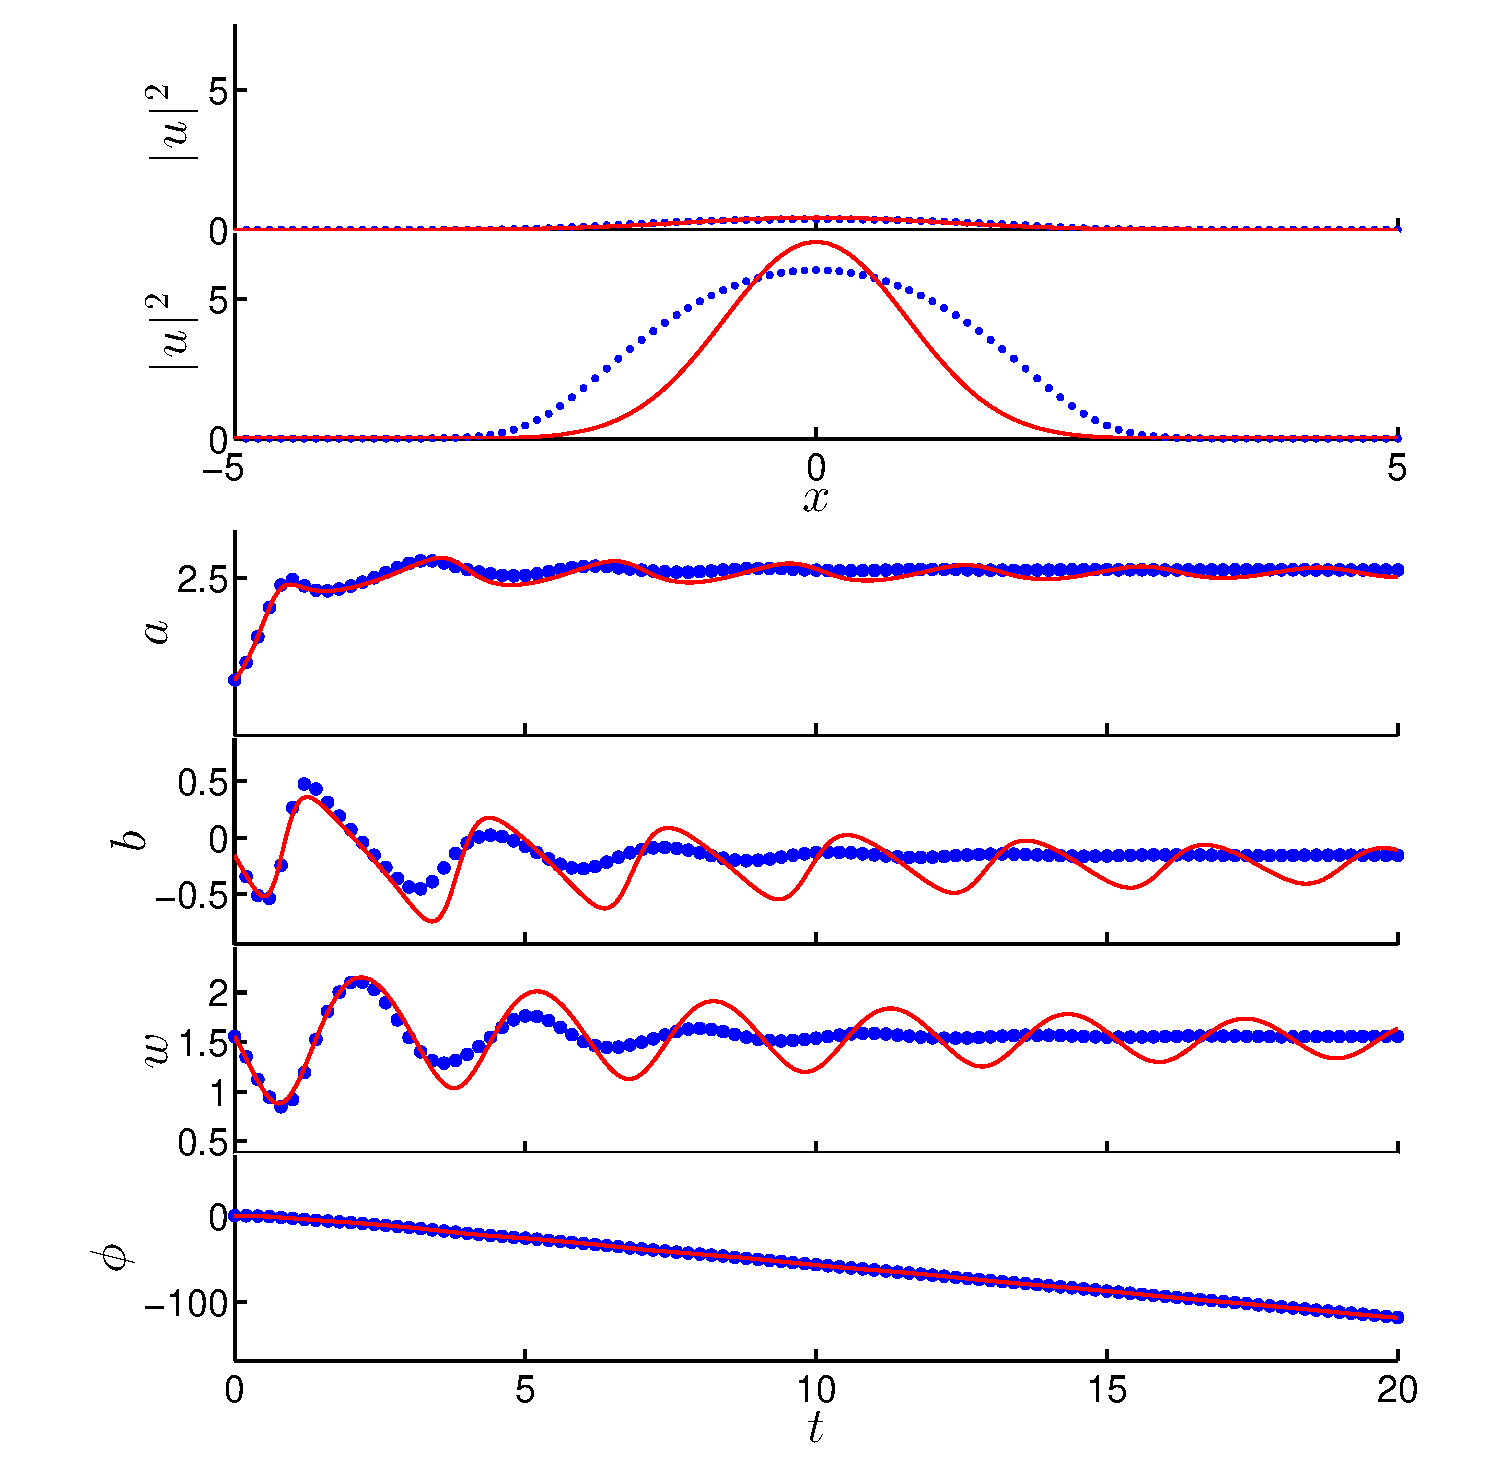
\includegraphics[width=0.8\textwidth]{Figures/Fig3a_P4_increase_v2.eps}}
  \rule{35em}{0.5pt}
\caption[Exciton-Polariton Above Equilibrium]{Evolution of the ground state of Eq.~(\ref{eq:NLSP}) starting below equilibrium in the presence of a linear spatially dependent gain (\ref{eq:gainP}) with
$\alpha =2$ and $\beta=2$, and density dependent loss of strength 
$\sigma =0.37$, as well as a harmonic potential (\ref{eq:potP}) 
of strength $\Omega = \sqrt{2}$.
%
To craft initial conditions with amplitudes below the equilibrium amplitudes we first computed the
steady state of the NLS (\ref{eq:NLSP}) which,
after projection, using least-squares fitting, into the Gaussian ansatz 
(\ref{eq:GaussAnsatz}) yields the following initial parameters:
amplitude: $a(0)= 0.6608 = a_e/4$ (four times {\em smaller} than the equilibrium solution), width:  $w(0)=1.5583$, chirp: $b(0) = -0.1563$, and phase: $\phi(0)=0.2415$.
%
Depicted are the comparison of the NCVA approximation of Eq.~(\ref{eq:NCVAP})
(red lines) with the full, numerical, NLS evolution of Eq.~(\ref{eq:NLSP})
(blue dots).
%
The top two panels depict the density $|u|^2$ at the initial time (top subpanel)
and at time $t=50$ (second subpanel).
%
The bottom four subpanels depict the evolution of the NCVA ansatz parameters
$a$, $b$, $w$, and $\phi$. For the full NLS evolution the parameters are
extracted by projecting the current solution into the NCVA ansatz using 
least-squares fitting.
\label{fig4}}
\end{figure}

\begin{figure}[htbp]
\centering
\centerline{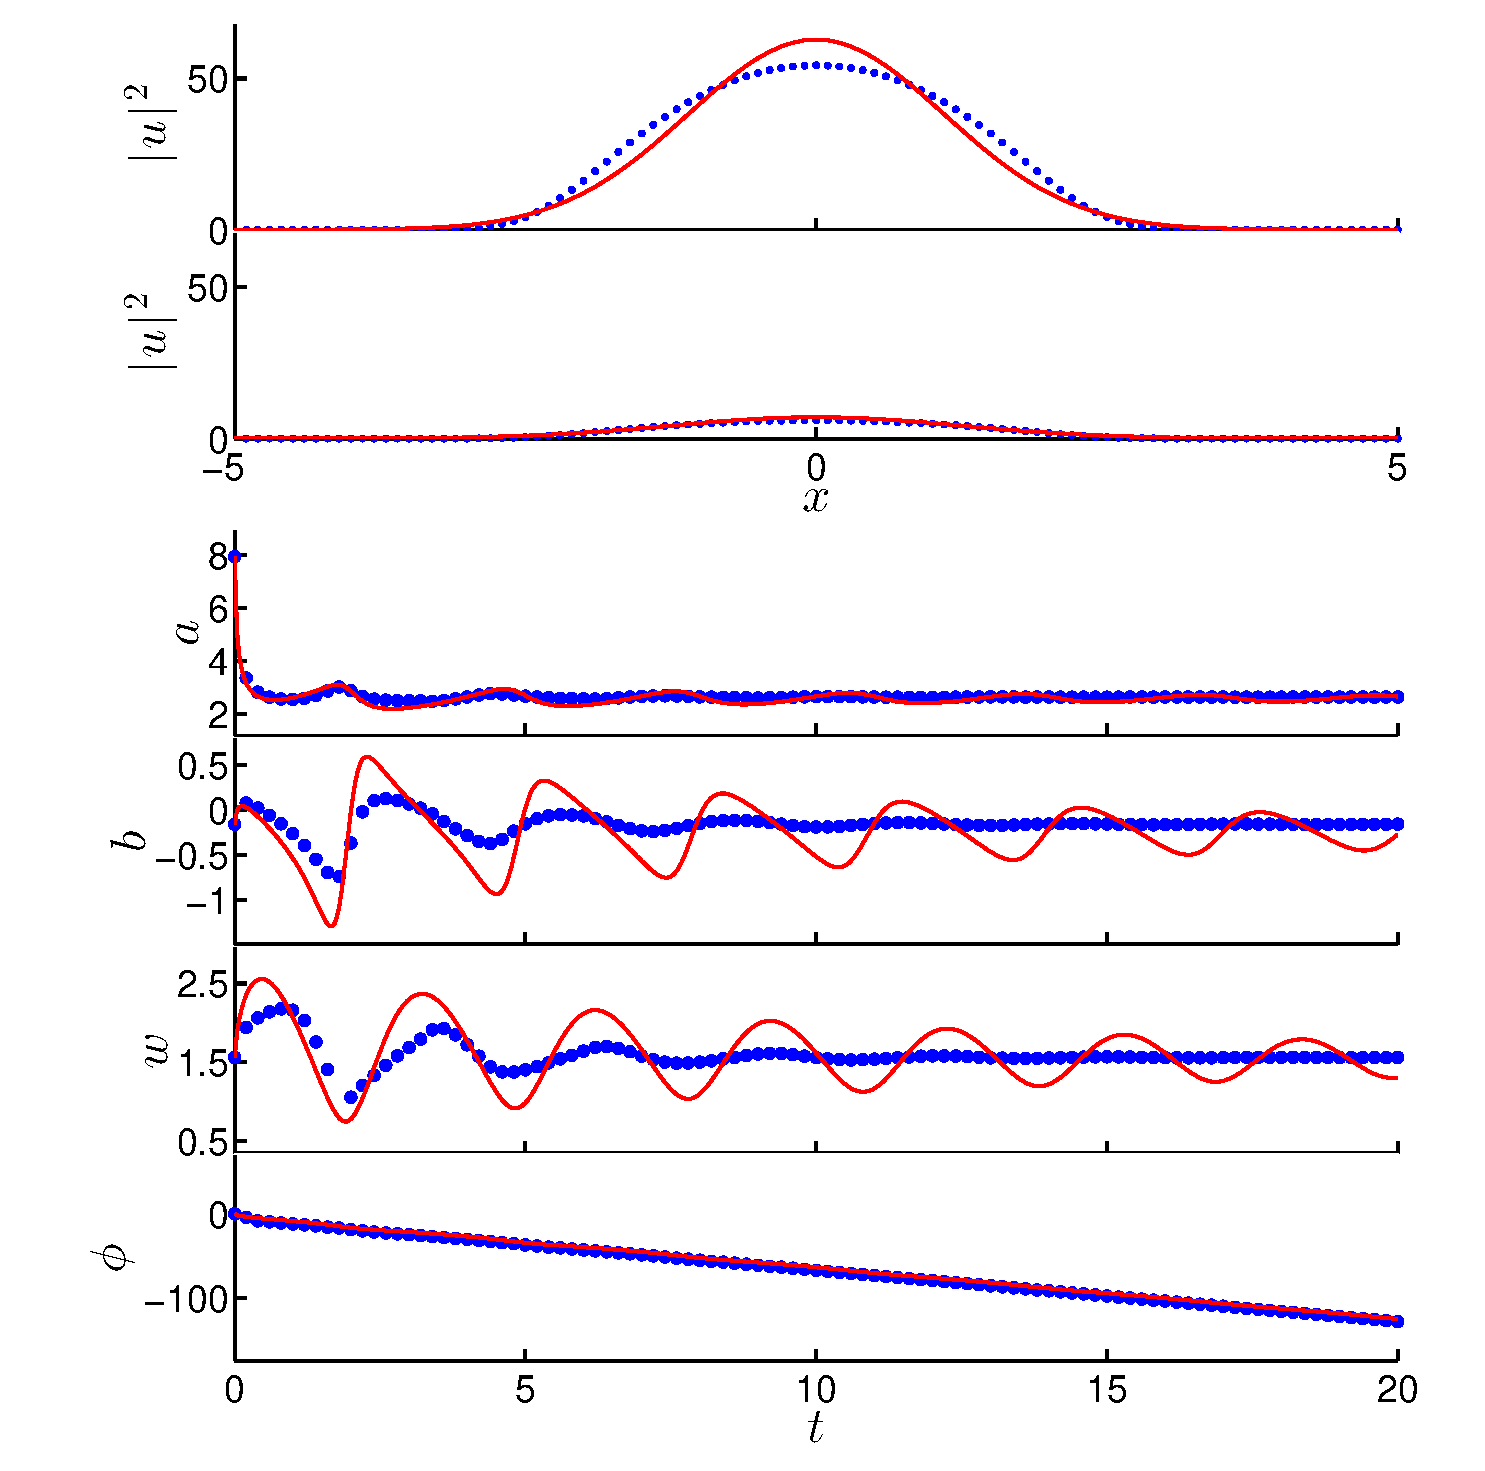
\includegraphics[width=0.8\textwidth]{Figures/Fig3b_P4_decrease_v2N.eps}}
  \rule{35em}{0.5pt}
\caption[Exciton-Polariton Below Equilibrium]{
Evolution of the ground state of Eq.~(\ref{eq:NLSP}) with the same coefficients as Fig.~\ref{fig4} starting above equilibrium
%in the presence of a linear spatially
%dependent gain (\ref{eq:gainP}) with
%$\alpha =2$ and $\beta=2$, and density dependent loss of strength 
%$\sigma =0.37$, as well as a harmonic potential (\ref{eq:potP}) 
%of strength $\Omega = \sqrt{2}$.
%
%To craft initial conditions with amplitudes above the equilibrium amplitudes we first computed the
%steady state of the NLS (\ref{eq:NLSP}) which,
%after projection, using least-squares fitting, into the Gaussian ansatz 
%(\ref{eq:GaussAnsatz}) yields the following initial parameters:
%amplitude: 
$a(0)= 7.9292 = 3 a_e$ (three times {\em larger}  than the equilibrium solution), width:  $w(0)=1.5583$, chirp: $b(0) = -0.1563$, and phase: $\phi(0)=0.2415$.
%
The layout of the panels is the same as in the previous Fig.~\ref{fig4}.
\label{fig5}}
\end{figure}

%\begin{figure}[htbp]
% \centering
%  \centerline{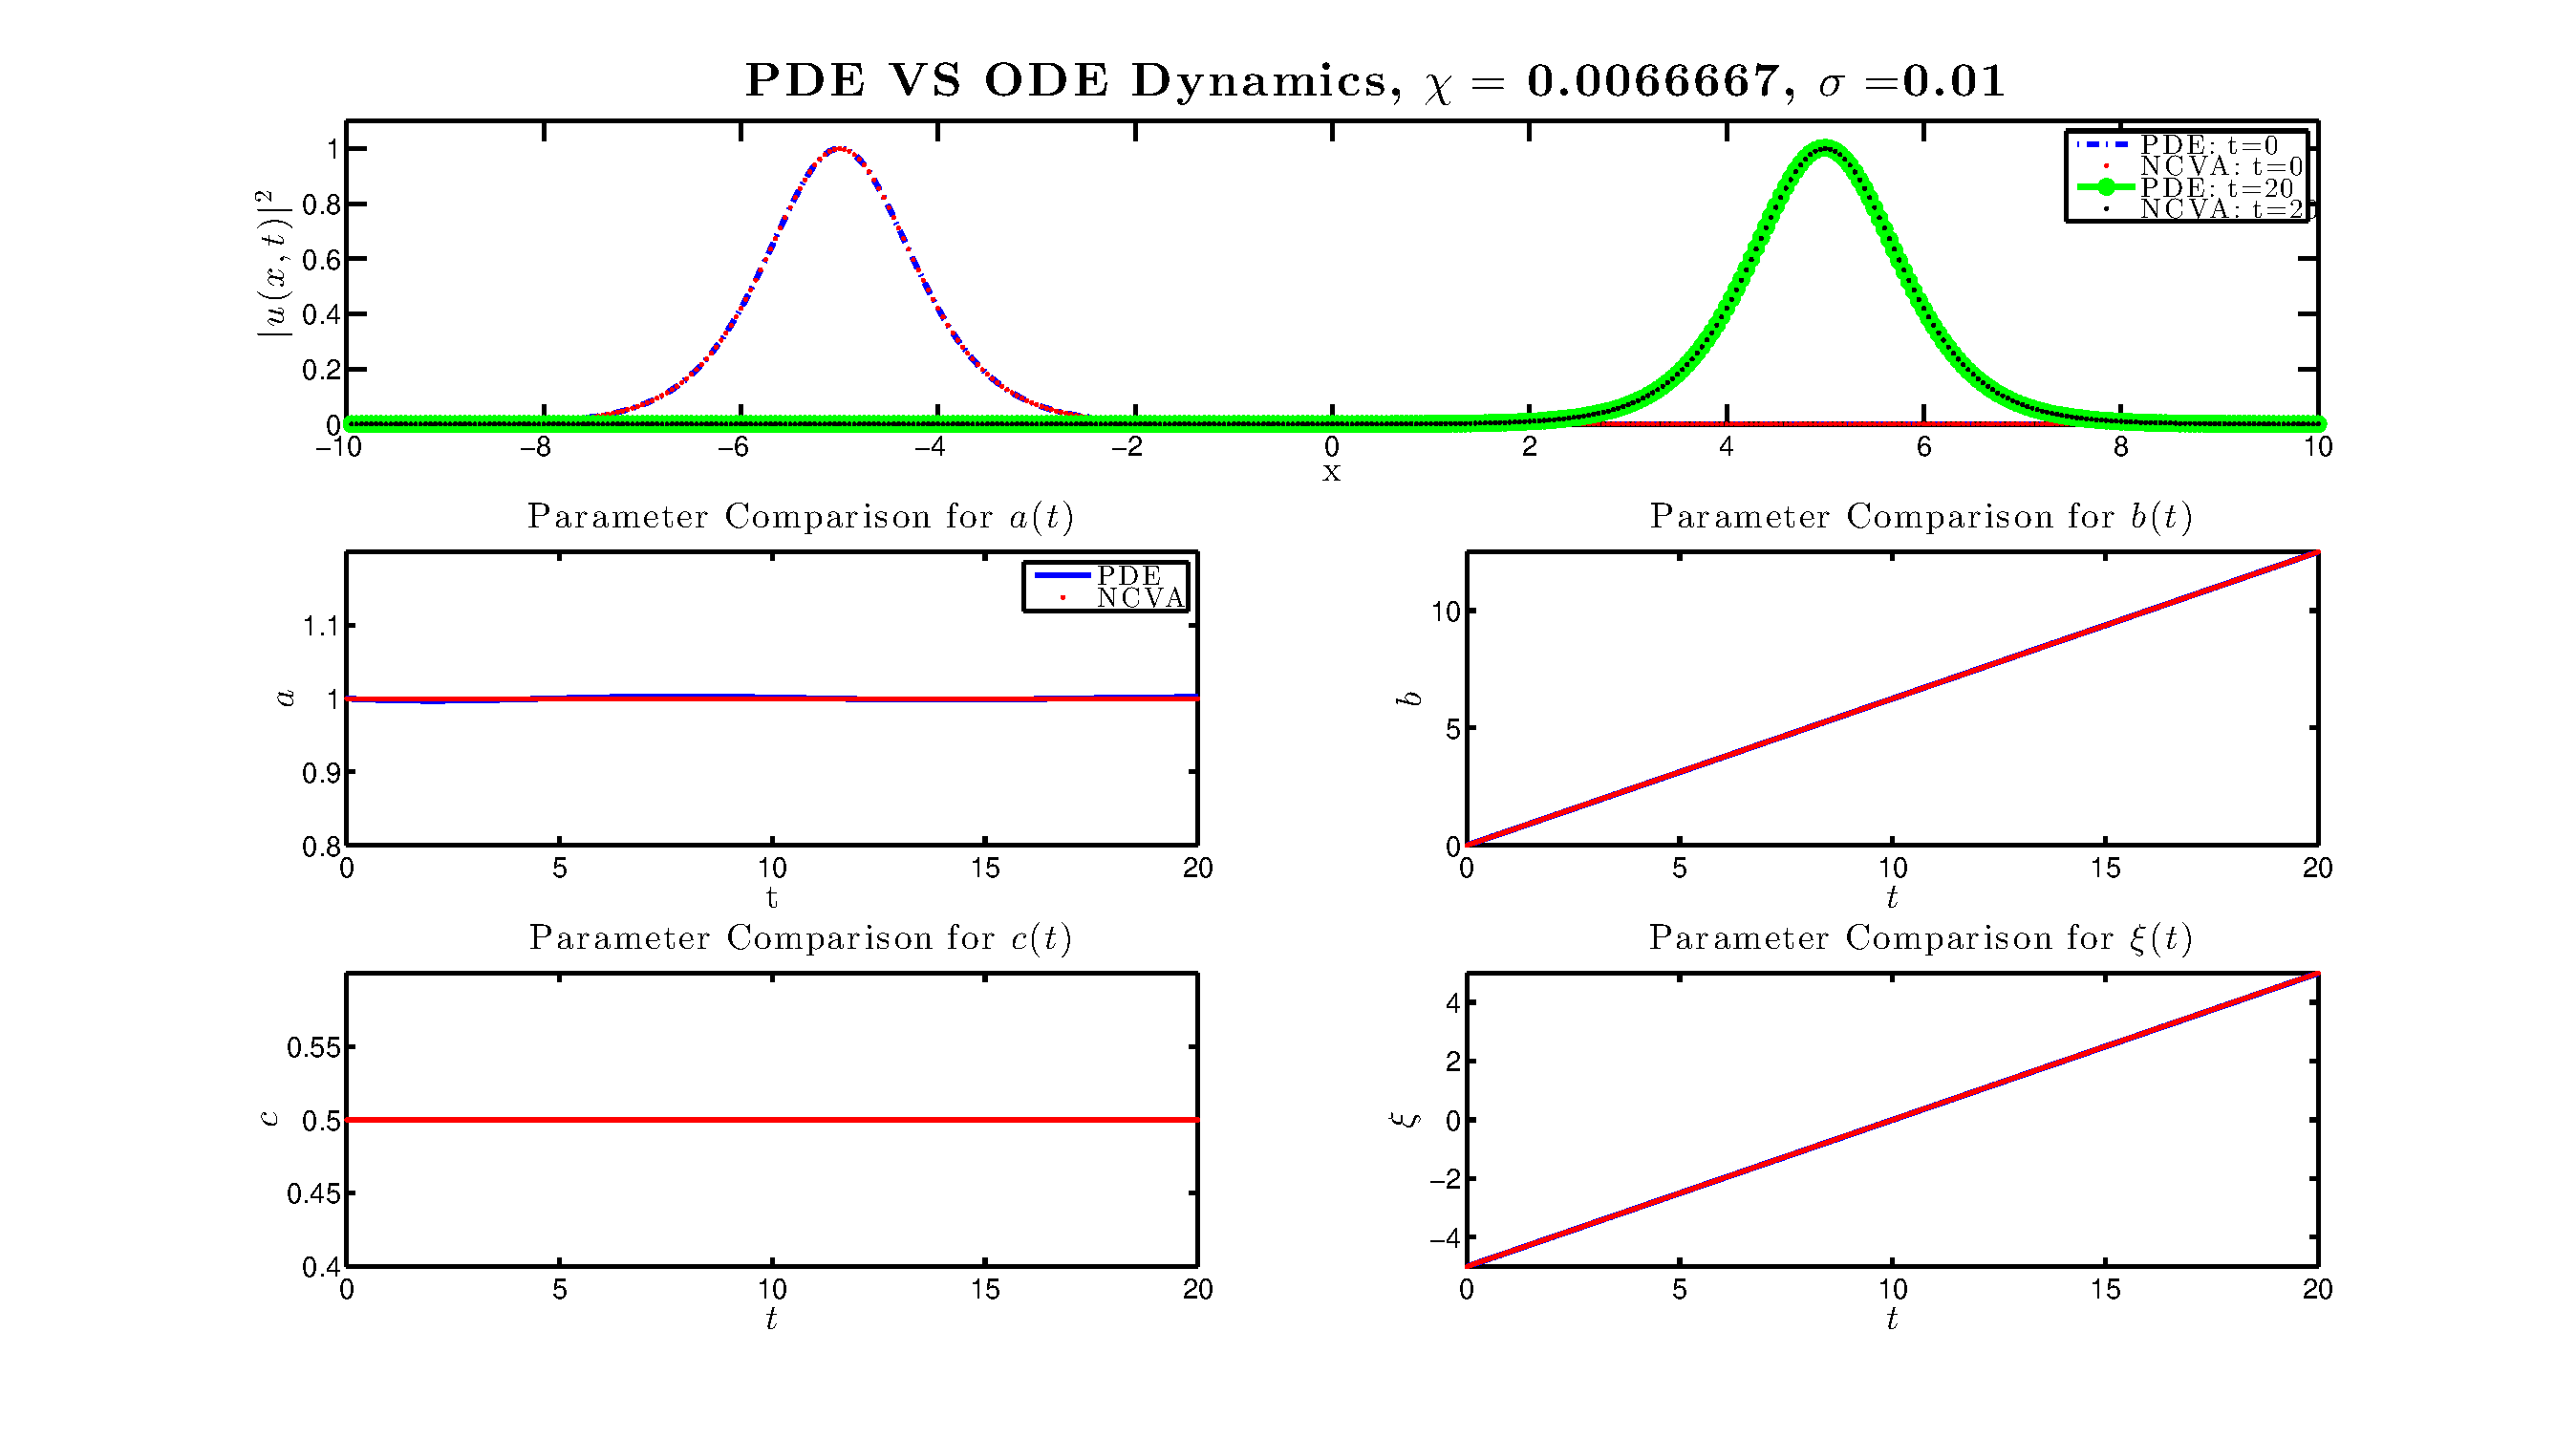
\includegraphics[width=1.2\textwidth, height=\textwidth]{EP001.eps}}
%  \rule{35em}{0.5pt}
%  \caption[Exciton-Polariton Condensate: NLS with Linear Gain $\sigma = 0.01$ and Density Dependent Loss $\chi=(2/3) \sigma$ ]{{\bf Exciton-Polariton Condensate:} Comparison of ODE dynamics for the parameters $a$, $b$, $c$, and $\xi$ between forward integration of the PDE and the NCVA with $\chi=(2/3) \sigma$ and $\sigma = 0.01$.}
%   \label{fig:Ploss001}
%\end{figure}
%
%
%\begin{figure}[htbp]
%  \centering
%  \centerline{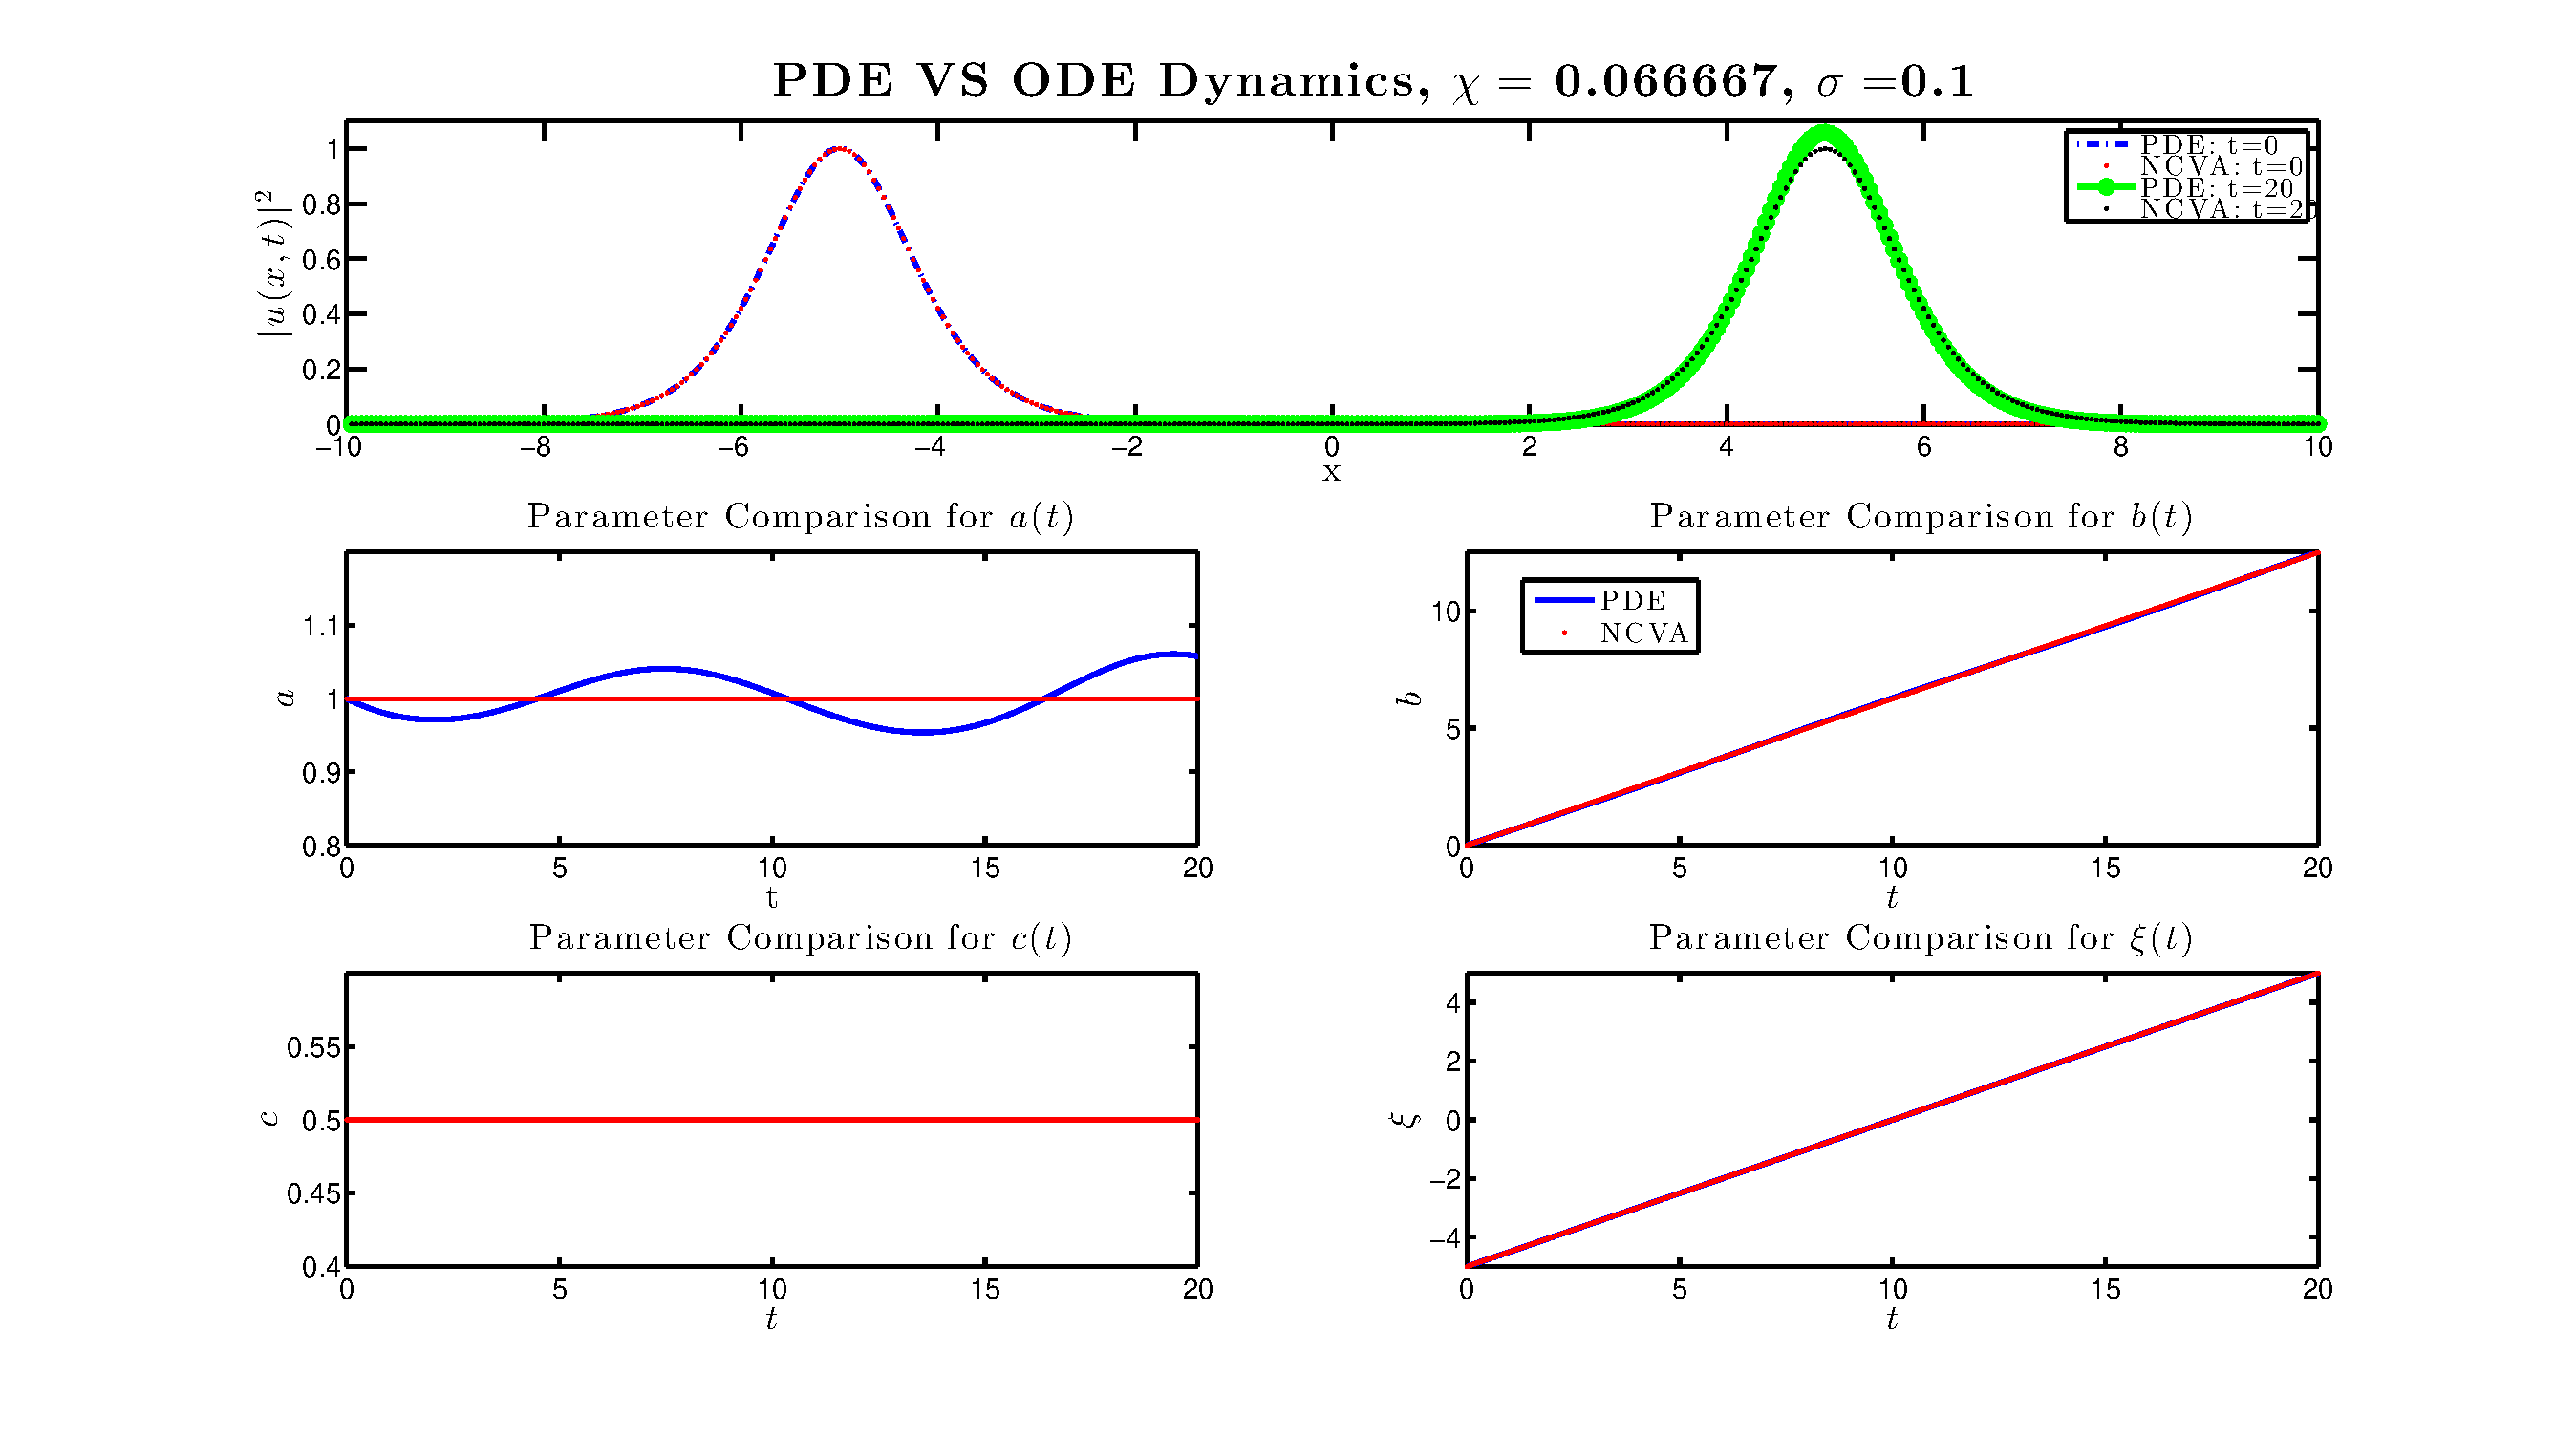
\includegraphics[width=1.2\textwidth, height=\textwidth]{EP01.eps}}
%  \rule{35em}{0.5pt}
%  \caption[Exciton-Polariton Condensate: NLS with Linear Gain $\sigma = 0.1$ and Density Dependent Loss $\chi=(2/3) \sigma$]{{\bf Exciton-Polariton Condensate:} Comparison of ODE dynamics for the parameters $a$, $b$, $c$, and $\xi$ between forward integration of the PDE and the NCVA with $\chi=(2/3) \sigma$ and $\sigma = 0.1$.}
%   \label{fig:Ploss01}
%\end{figure}
%
%\begin{figure}[htbp]
%\centering
%\begin{subfigure}[t]{0.49\textwidth}
%  		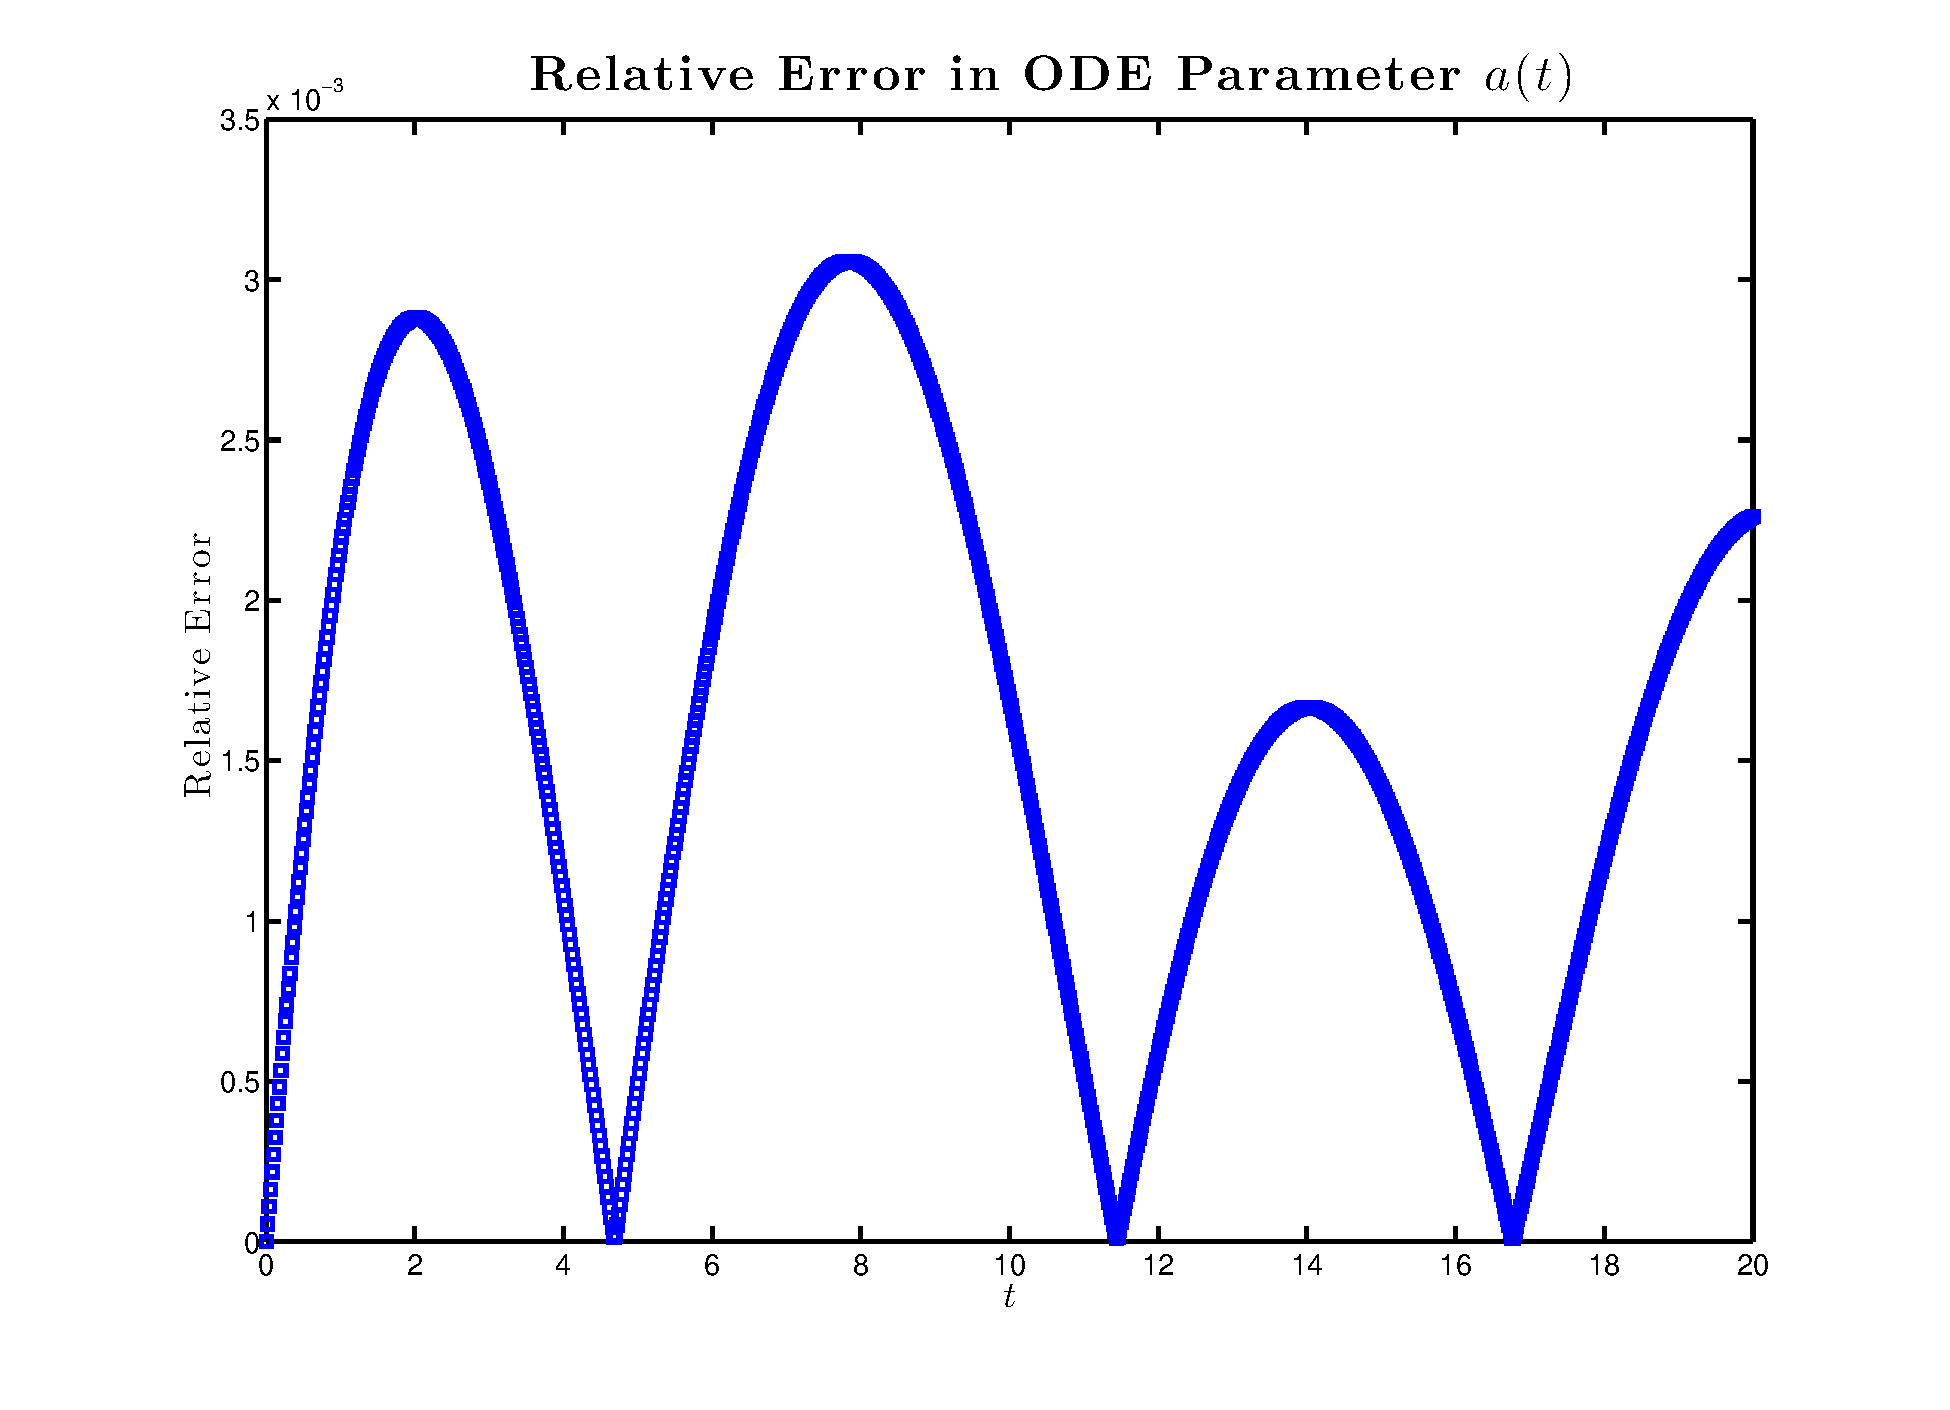
\includegraphics[width=\textwidth, height = \textwidth]{EP001relativeerror.eps}
%	         \caption{Relative error between NCVA and PDE parameter $a(t)$ values for $\sigma=0.01$.}
%	         \label{fig:PLoss001Err}
%	     \end{subfigure}
%  \begin{subfigure}[t]{0.49\textwidth}
%  		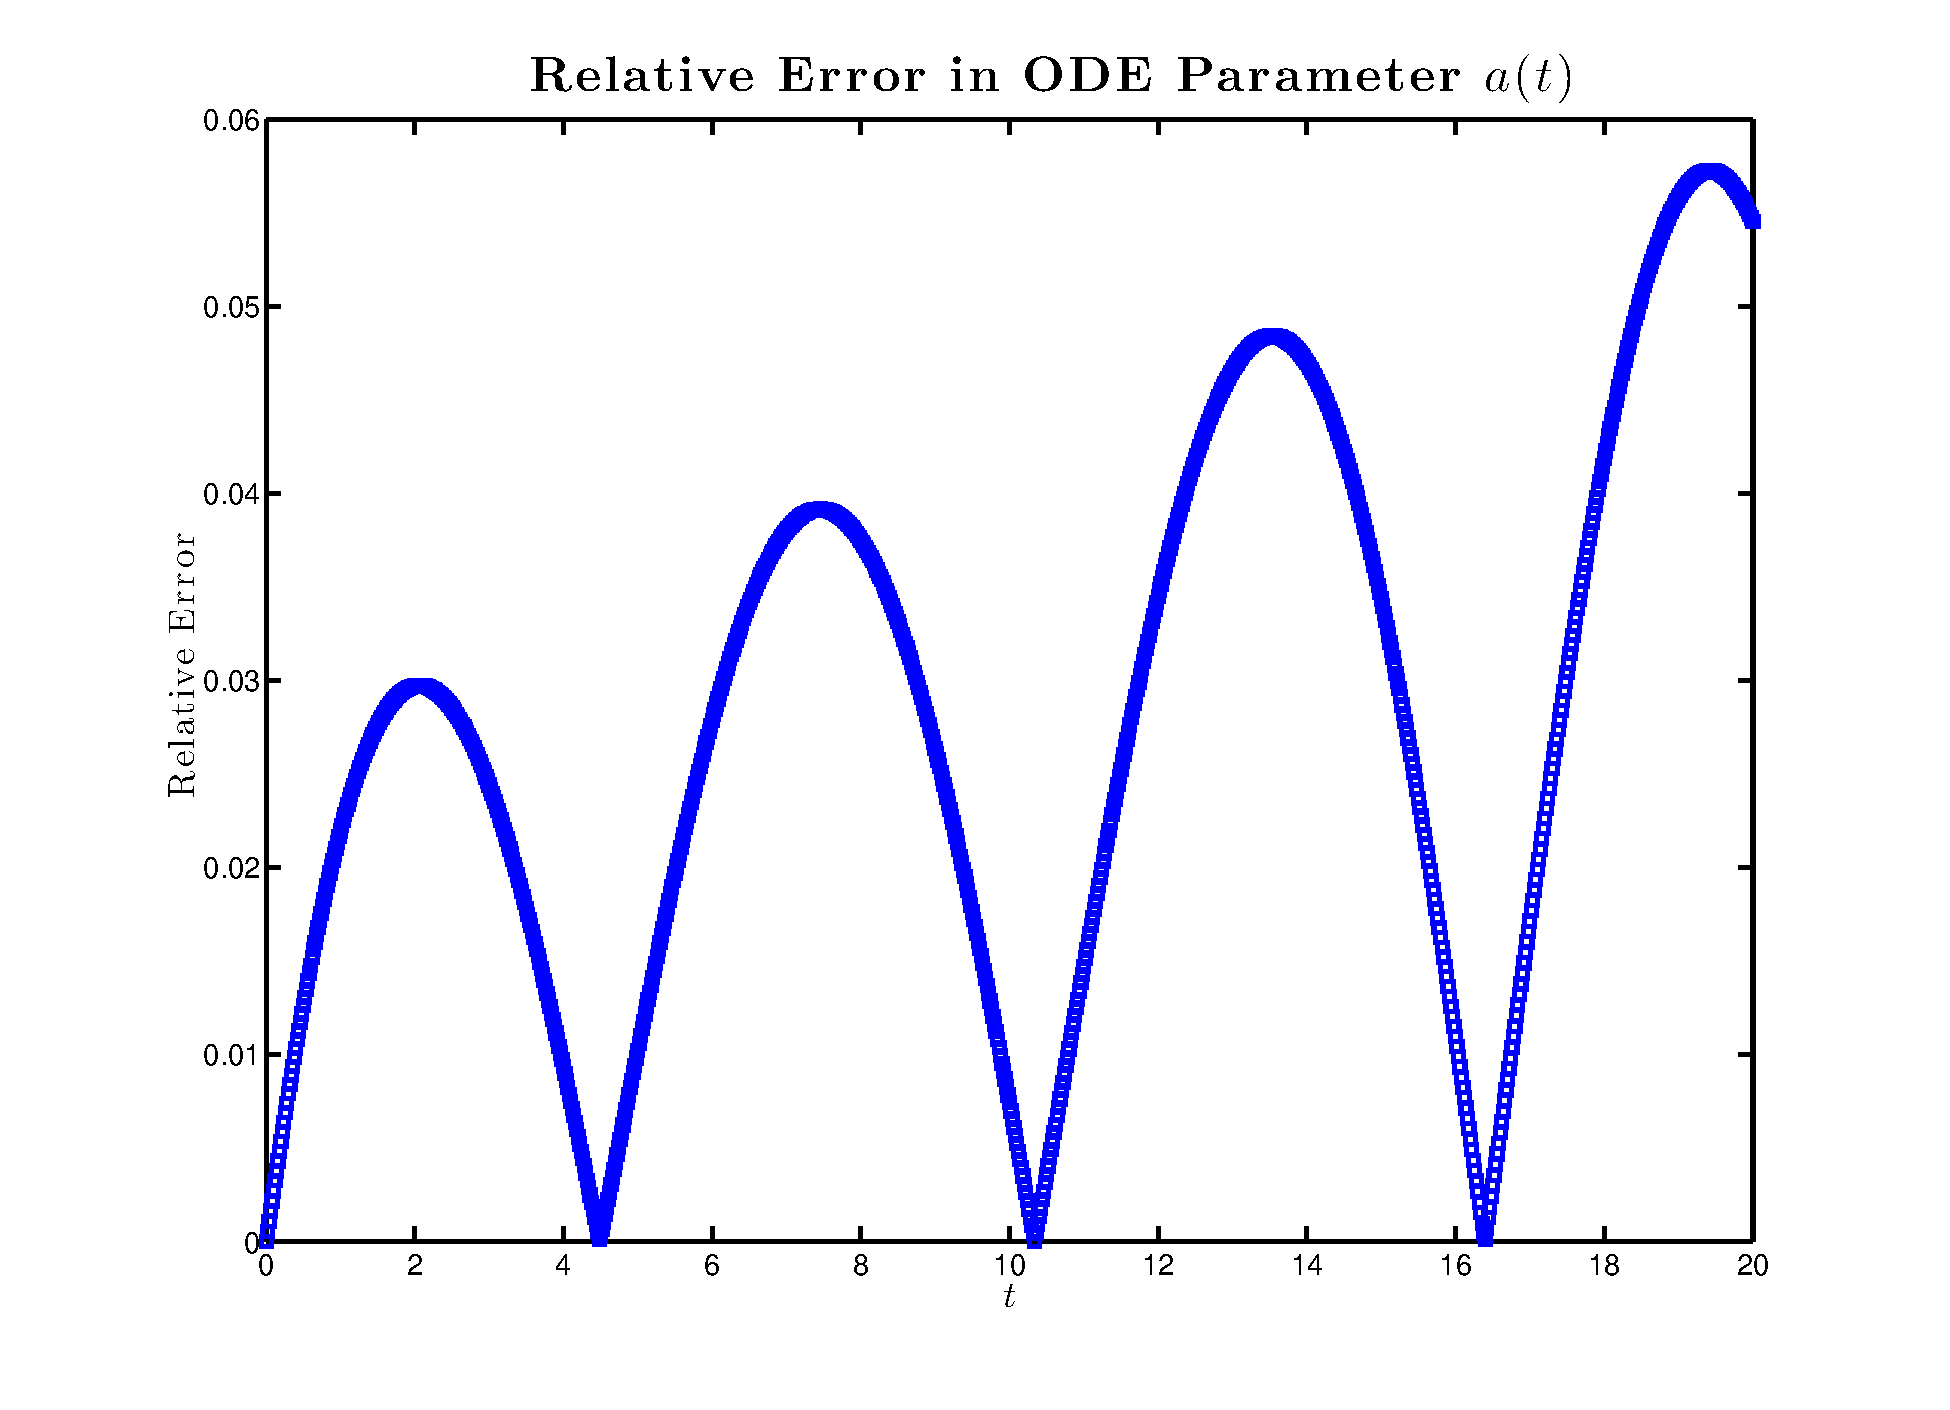
\includegraphics[width= \textwidth, height = \textwidth]{EP01relativeerror.eps}  
%	          \caption{Relative error between NCVA and PDE parameter $a(t)$ values for $\sigma=0.1$.}
%	         \label{fig:PLoss01Err}
%	    \end{subfigure} 
%  \rule{35em}{0.5pt}
%   \caption[Relative Error in Amplitude for Exciton-Polariton Condensate: NLS with Linear Gain and Density Dependent Loss $\chi=(2/3) \sigma$]{{\bf Exciton-Polariton Condensate:} Amplitude parameter $a(t)$ relative error for $\chi=(2/3) \sigma$ where (A) $\sigma=0.01$ and (B) $\sigma=0.1$.}
%   \label{fig:PlossA}
%\end{figure}

%\clearpage
%
%The equilibrium shown in the examples above [Figs.~\ref{fig:Ploss001} and \ref{fig:Ploss01}] illustrate the dynamics of constant exciton pumping and loss of polaritons.  The interesting cases occur when the system is set far from the equilibrium point $a$ = 1.  We start with $a_0 = 1$ and show the soliton decaying to the equilibrium height $a$ = 1 over time $t\in[0,500]$ in Fig.~\ref{fig:Pdecay}.  The numerics were performed the same as above except $\xi_0 = -25$.  The relative error in the height for $a$ is on the order of $10^{-3}$ and increases to $10^{-2}$ over time in Fig.~\ref{fig:PdecayErr}.  The ODE and PDE solutions agree very well with the soliton solution decaying to the fixed point $a$ = 1.  The numerical oscillations of the PDE as time increases is believed to be an artifact of the fitting routine and more analysis will be performed.    
%
%In Fig.~\ref{fig:Pgain}, we start at a height $a$ less than the fixed point, $a_0$ = 0.5 such that the PDE and ODE solution will grow and eventually reach the fixed point $a =1$.  The same numeric parameters are used as before except $\xi_0 = -15$ and $t\in[0,300]$.  The relative error in the height for $a$ is on the order of $10^{-2}$ in Fig.~\ref{fig:PgainErr}.  The non-conserved system is well described by the NCVA equations of motion for the time-dependent parameters $a$, $b$, $c$, and $\xi$ especially when considering constant pumping in of excitons and decay (loss) of polaritons due to their short lifespan.

%\begin{figure}[htbp]
% \centering
%  \centerline{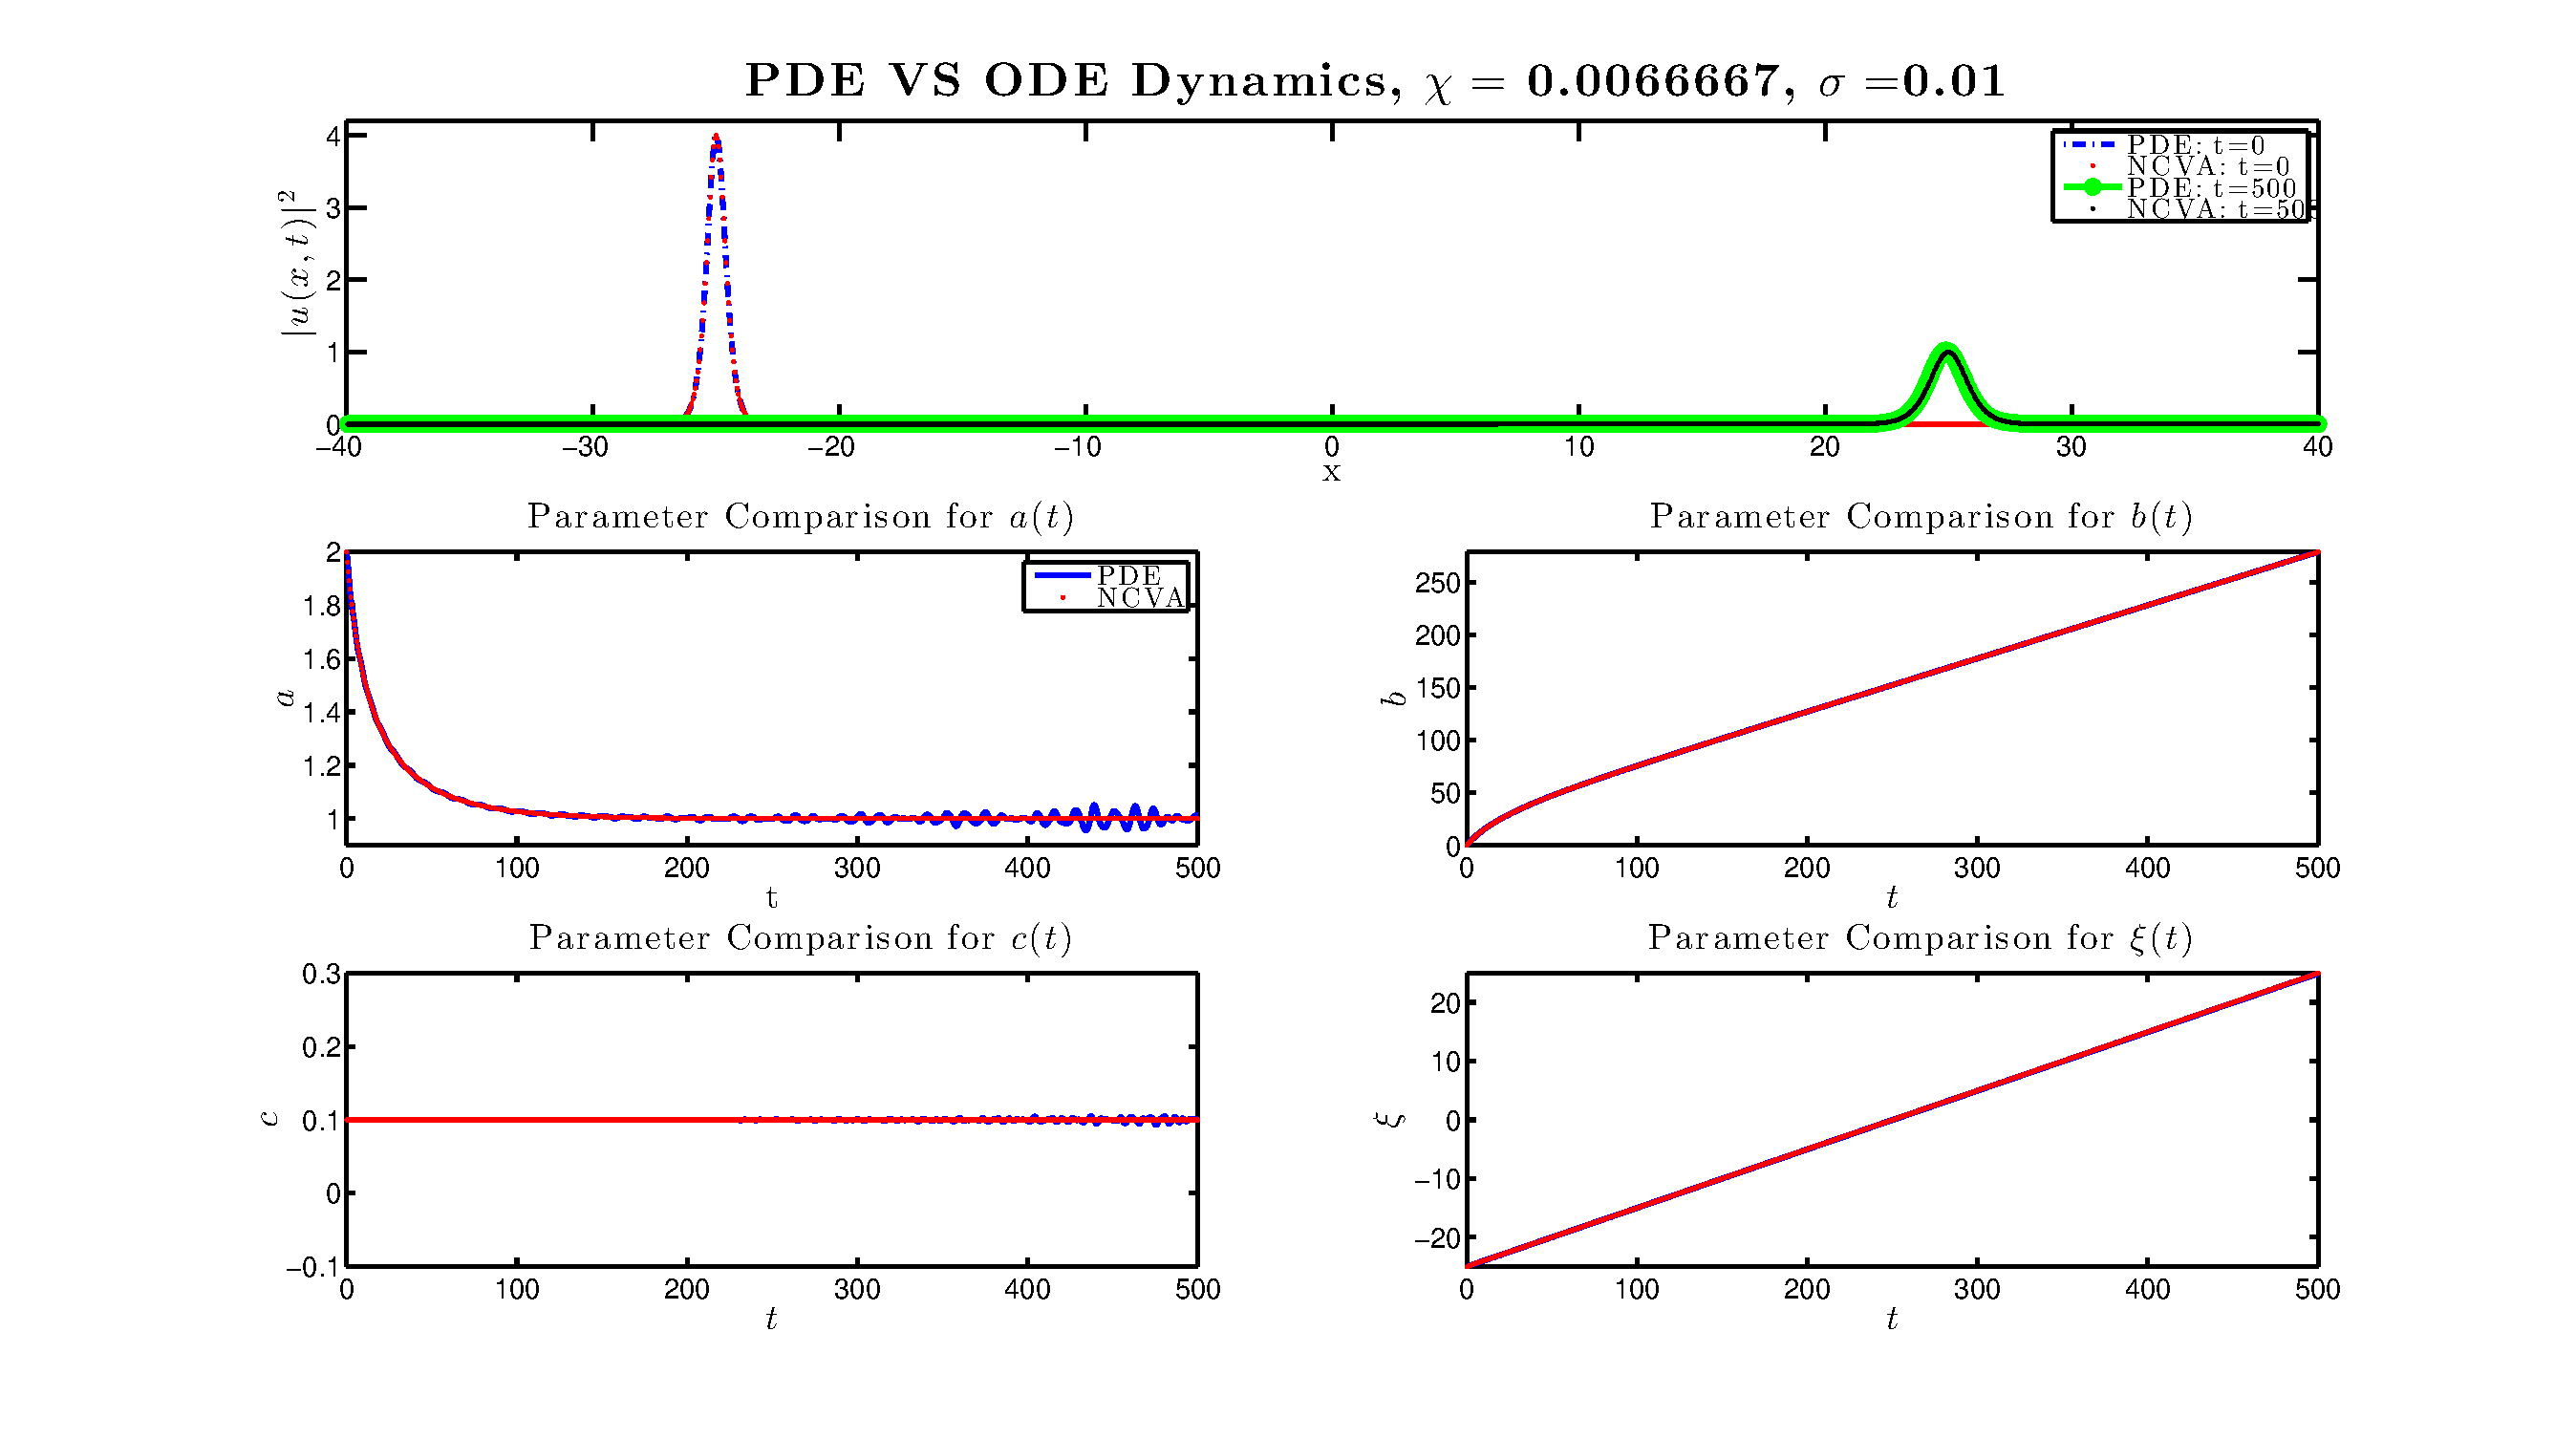
\includegraphics[width=1.2\textwidth, height=\textwidth]{EPdecay.eps}}
%  \rule{35em}{0.5pt}
%  \caption[Exciton-Polariton Condensate: NLS with Linear Gain $\sigma = 0.01$ and Density DependentLoss $\chi=(2/3) \sigma$ for $a_0 = 2$ ]{{\bf Exciton-Polariton Condensate:} Comparison of ODE dynamics for the parameters $a$, $b$, $c$, and $\xi$ between forward integration of the PDE and the NCVA with $\chi=(2/3) \sigma$ and $\sigma = 0.01$ starting at $a_0 = 2$.}
%   \label{fig:Pdecay}
%\end{figure}
%
%
%\begin{figure}[htbp]
%  \centering
%  \centerline{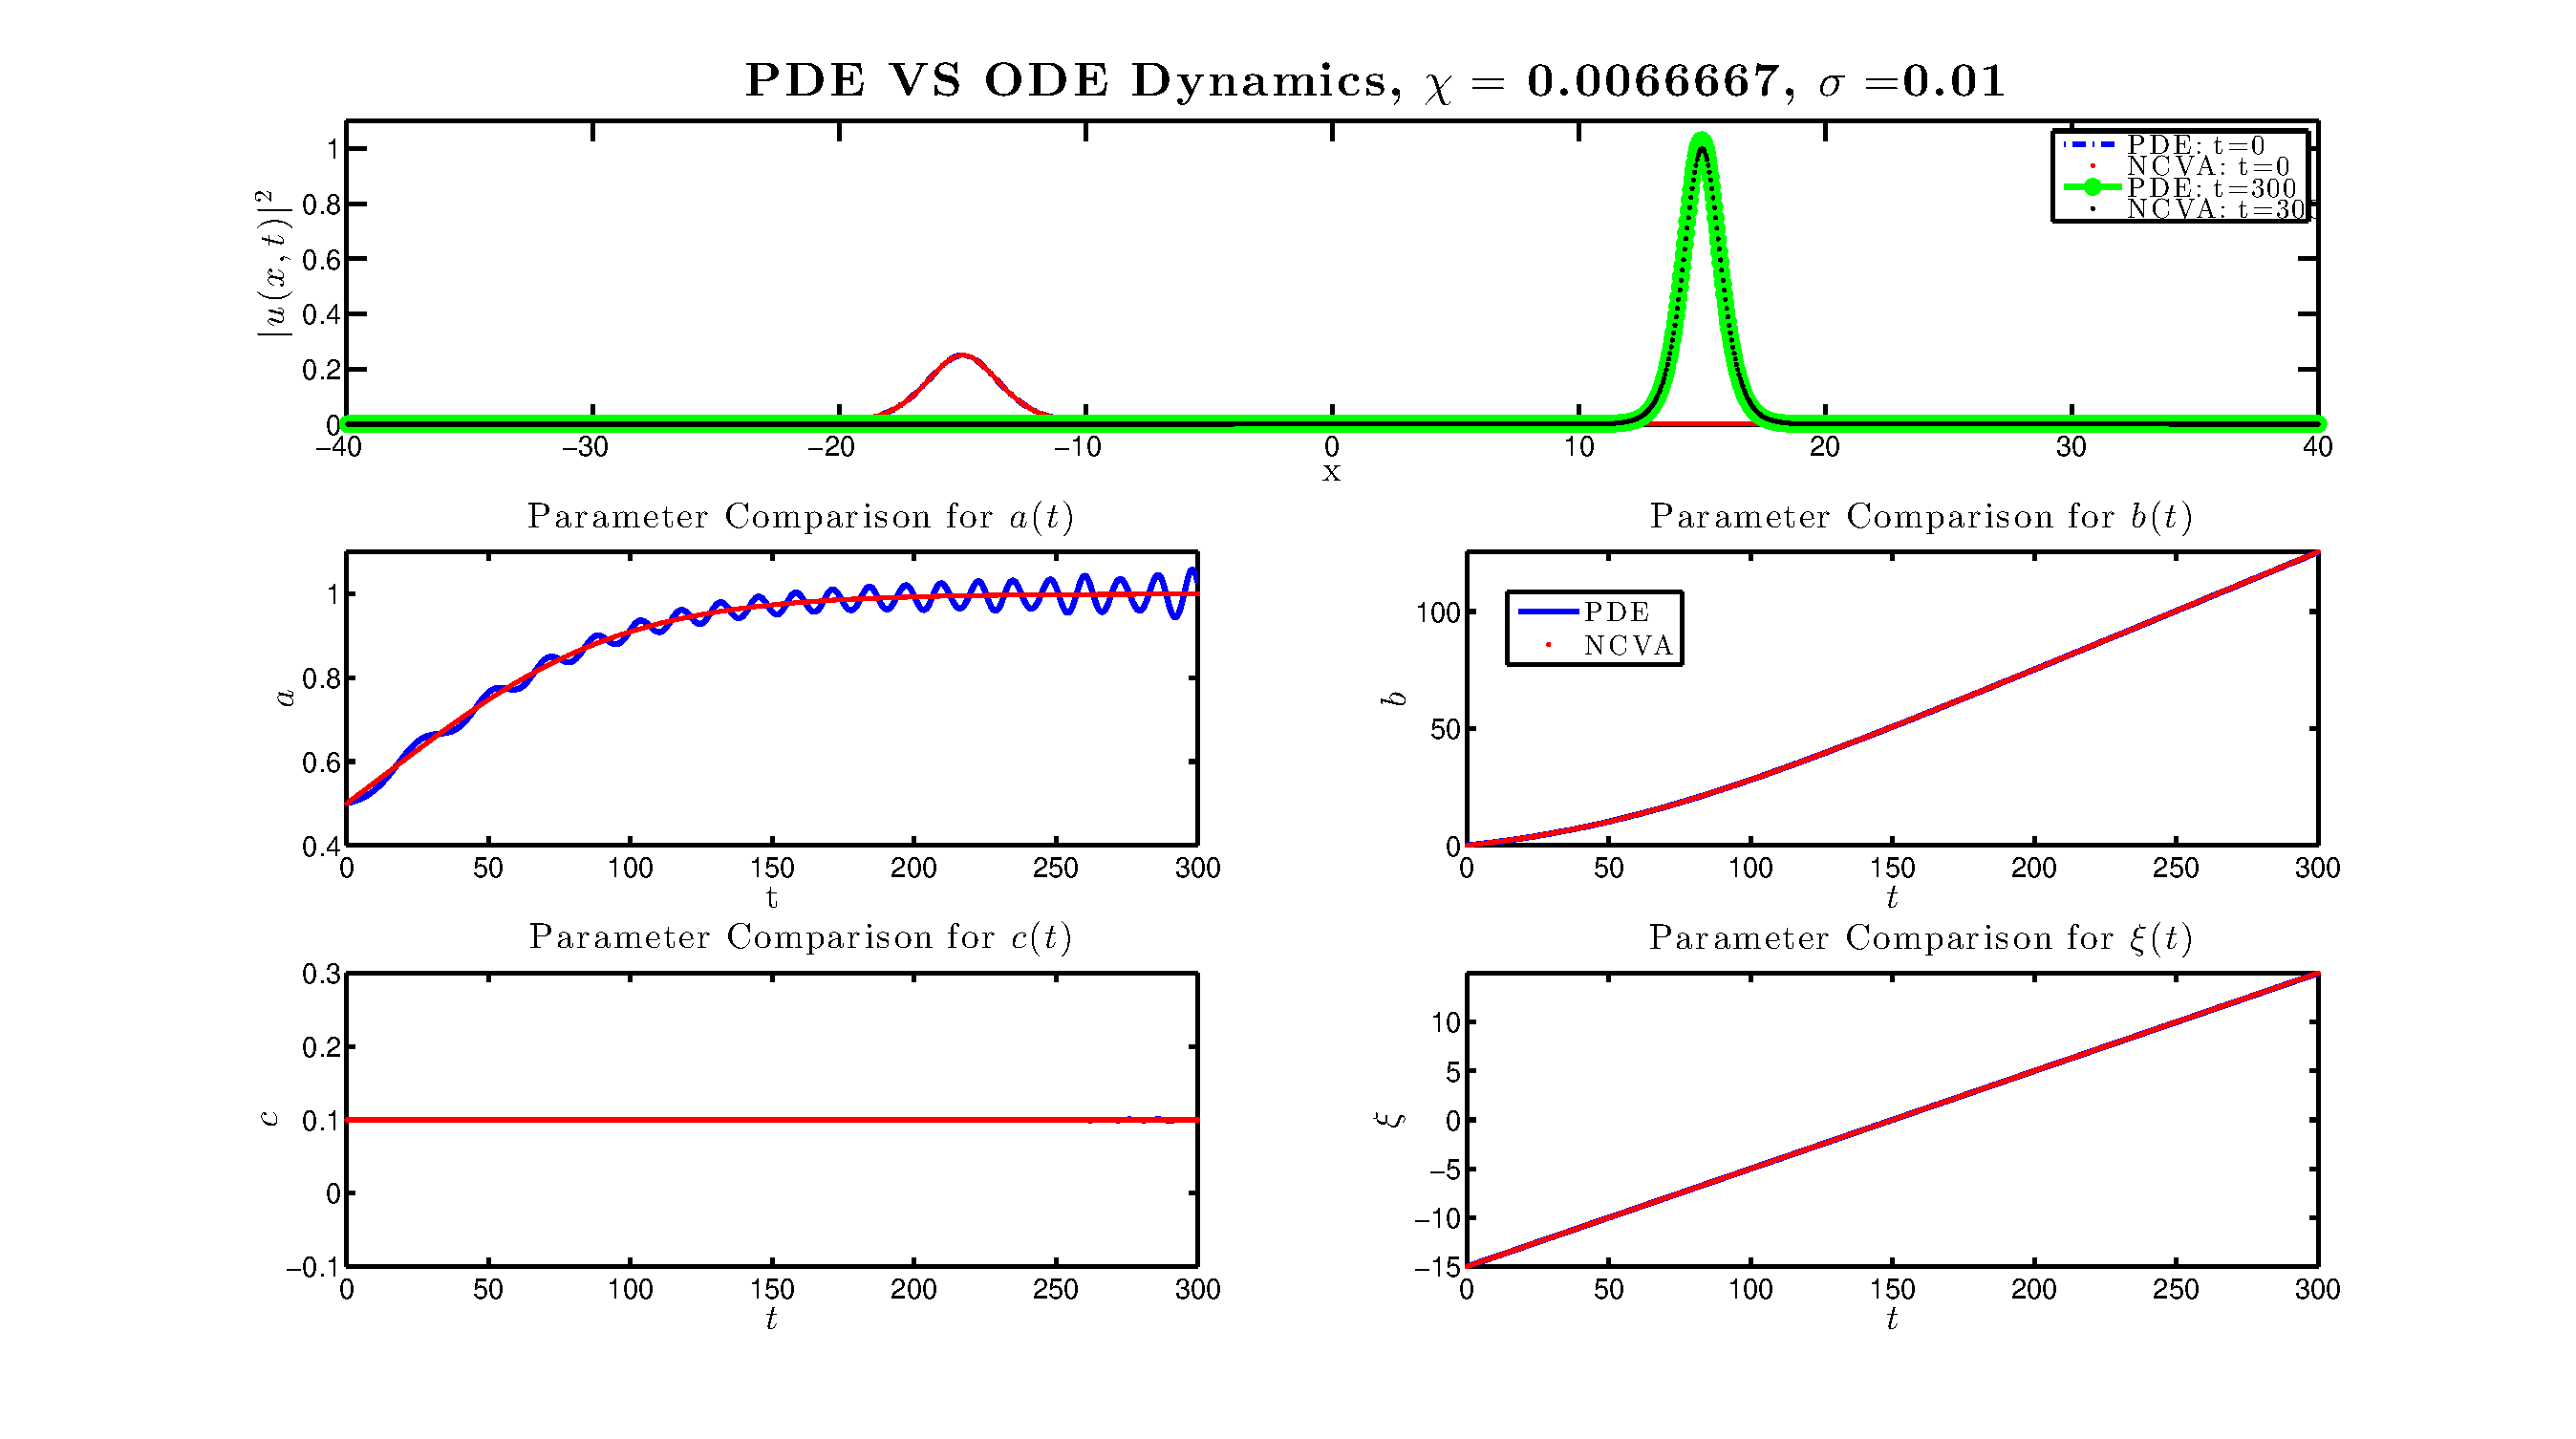
\includegraphics[width=1.2\textwidth, height=\textwidth]{EPgain.eps}}
%  \rule{35em}{0.5pt}
%  \caption[Exciton-Polariton Condensate: NLS with Linear Gain $\sigma = 0.01$ and Density Dependent Loss $\chi=(2/3) \sigma$ for $a_0 = 0.5$]{{\bf Exciton-Polariton Condensate:} Comparison of ODE dynamics for the parameters $a$, $b$, $c$, and $\xi$ between forward integration of the PDE and the NCVA with $\chi=(2/3) \sigma$ and $\sigma = 0.01$ starting at $a_0 = 0.5$.}
%   \label{fig:Pgain}
%\end{figure}
%
%\begin{figure}[htbp]
%\centering
%\begin{subfigure}[t]{0.49\textwidth}
%  		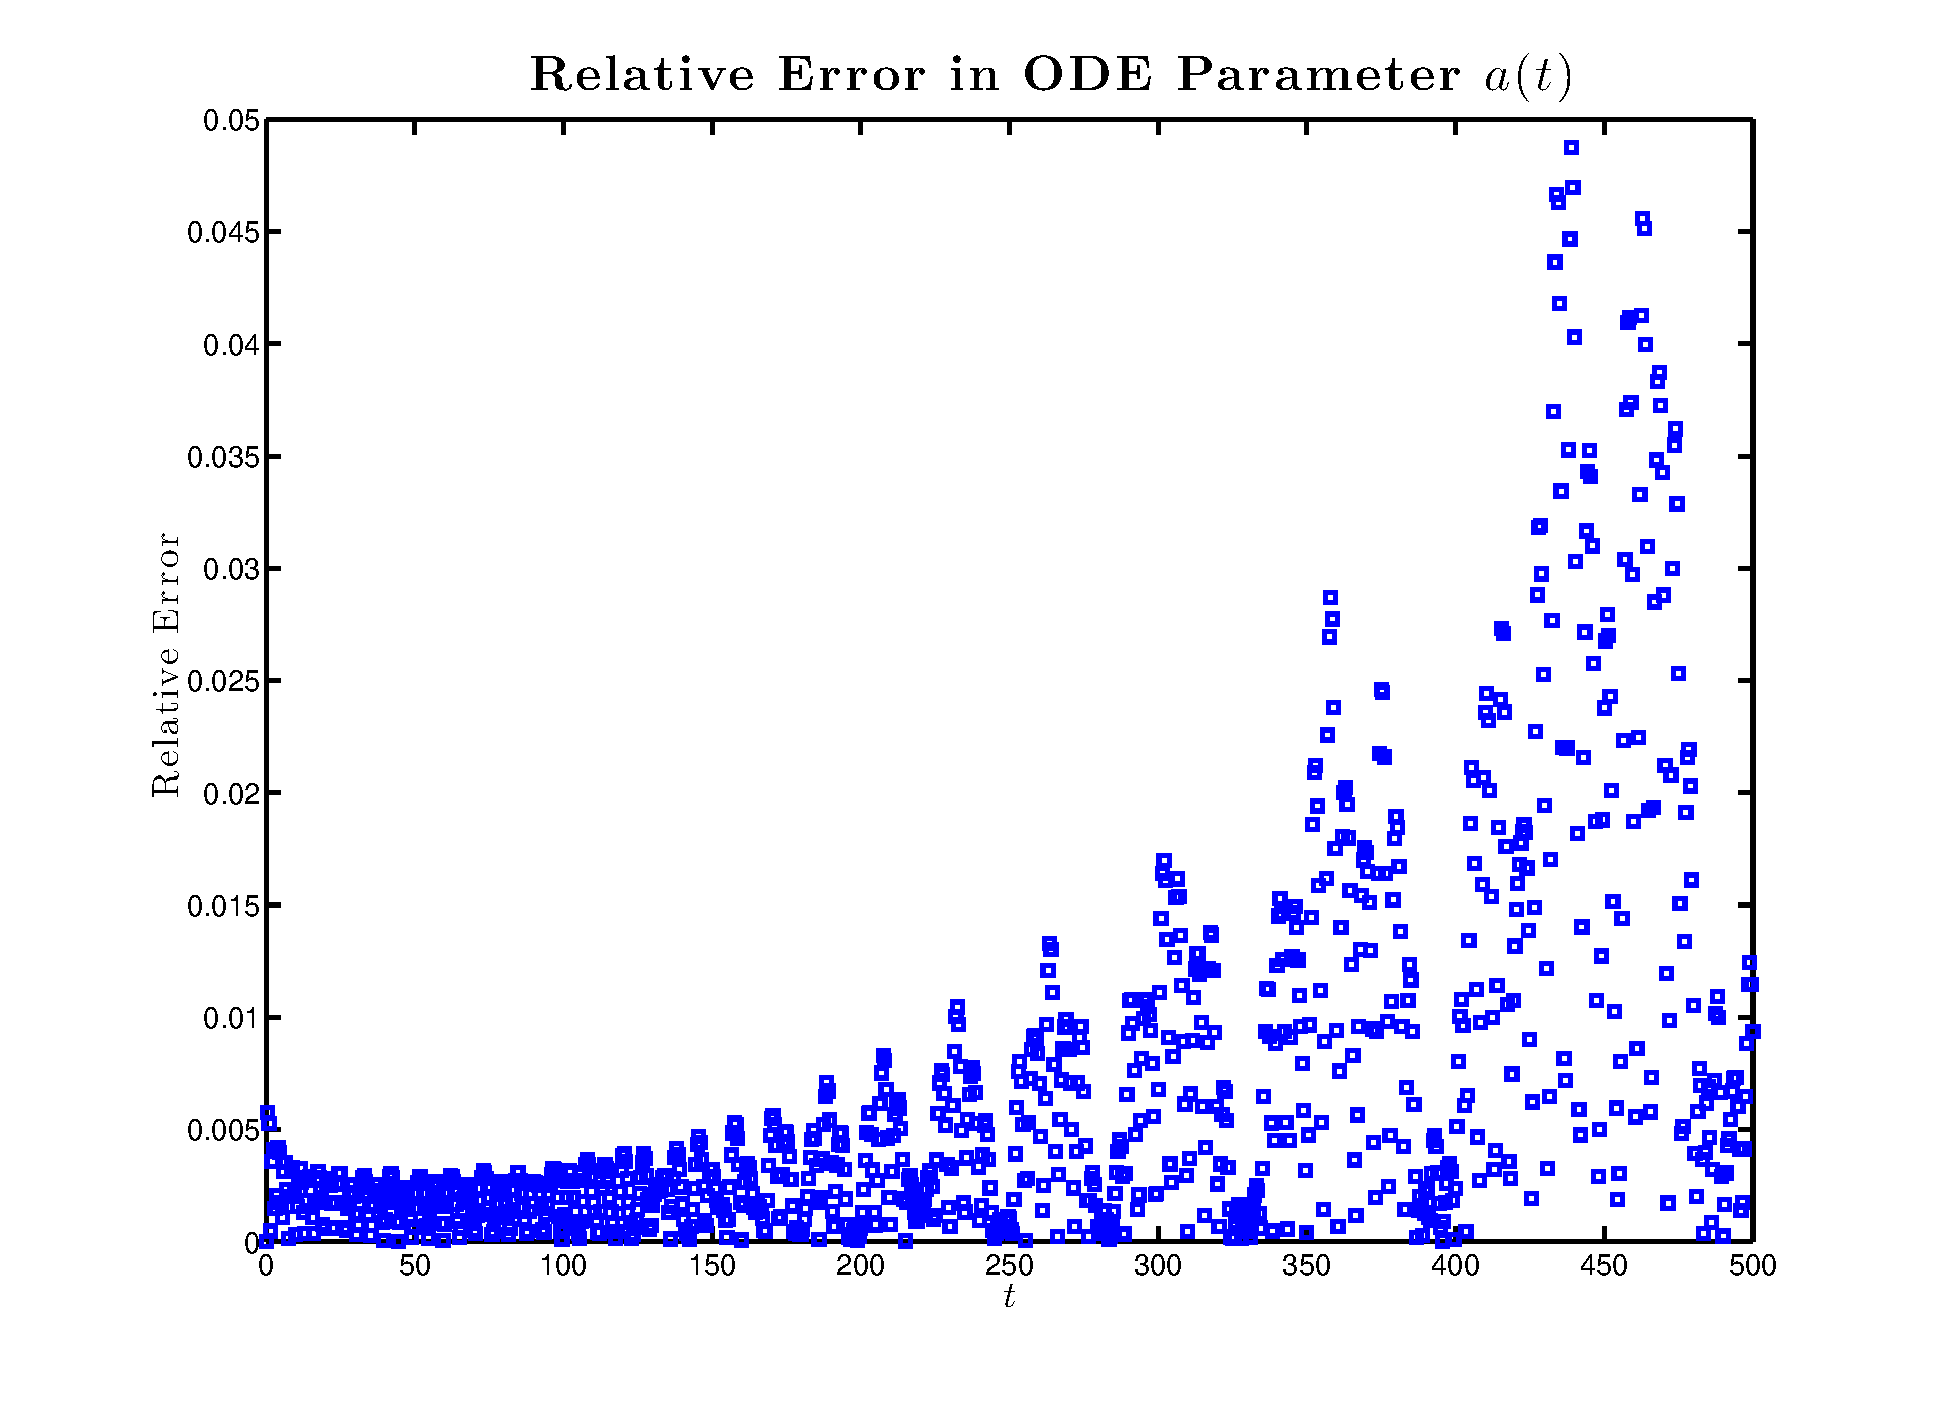
\includegraphics[width=\textwidth, height = \textwidth]{EPdecayrelativeerror.eps}
%	         \caption{Relative error between NCVA and PDE parameter $a(t)$ values for $a_0=2$.}
%	         \label{fig:PdecayErr}
%	     \end{subfigure}
%  \begin{subfigure}[t]{0.49\textwidth}
%  		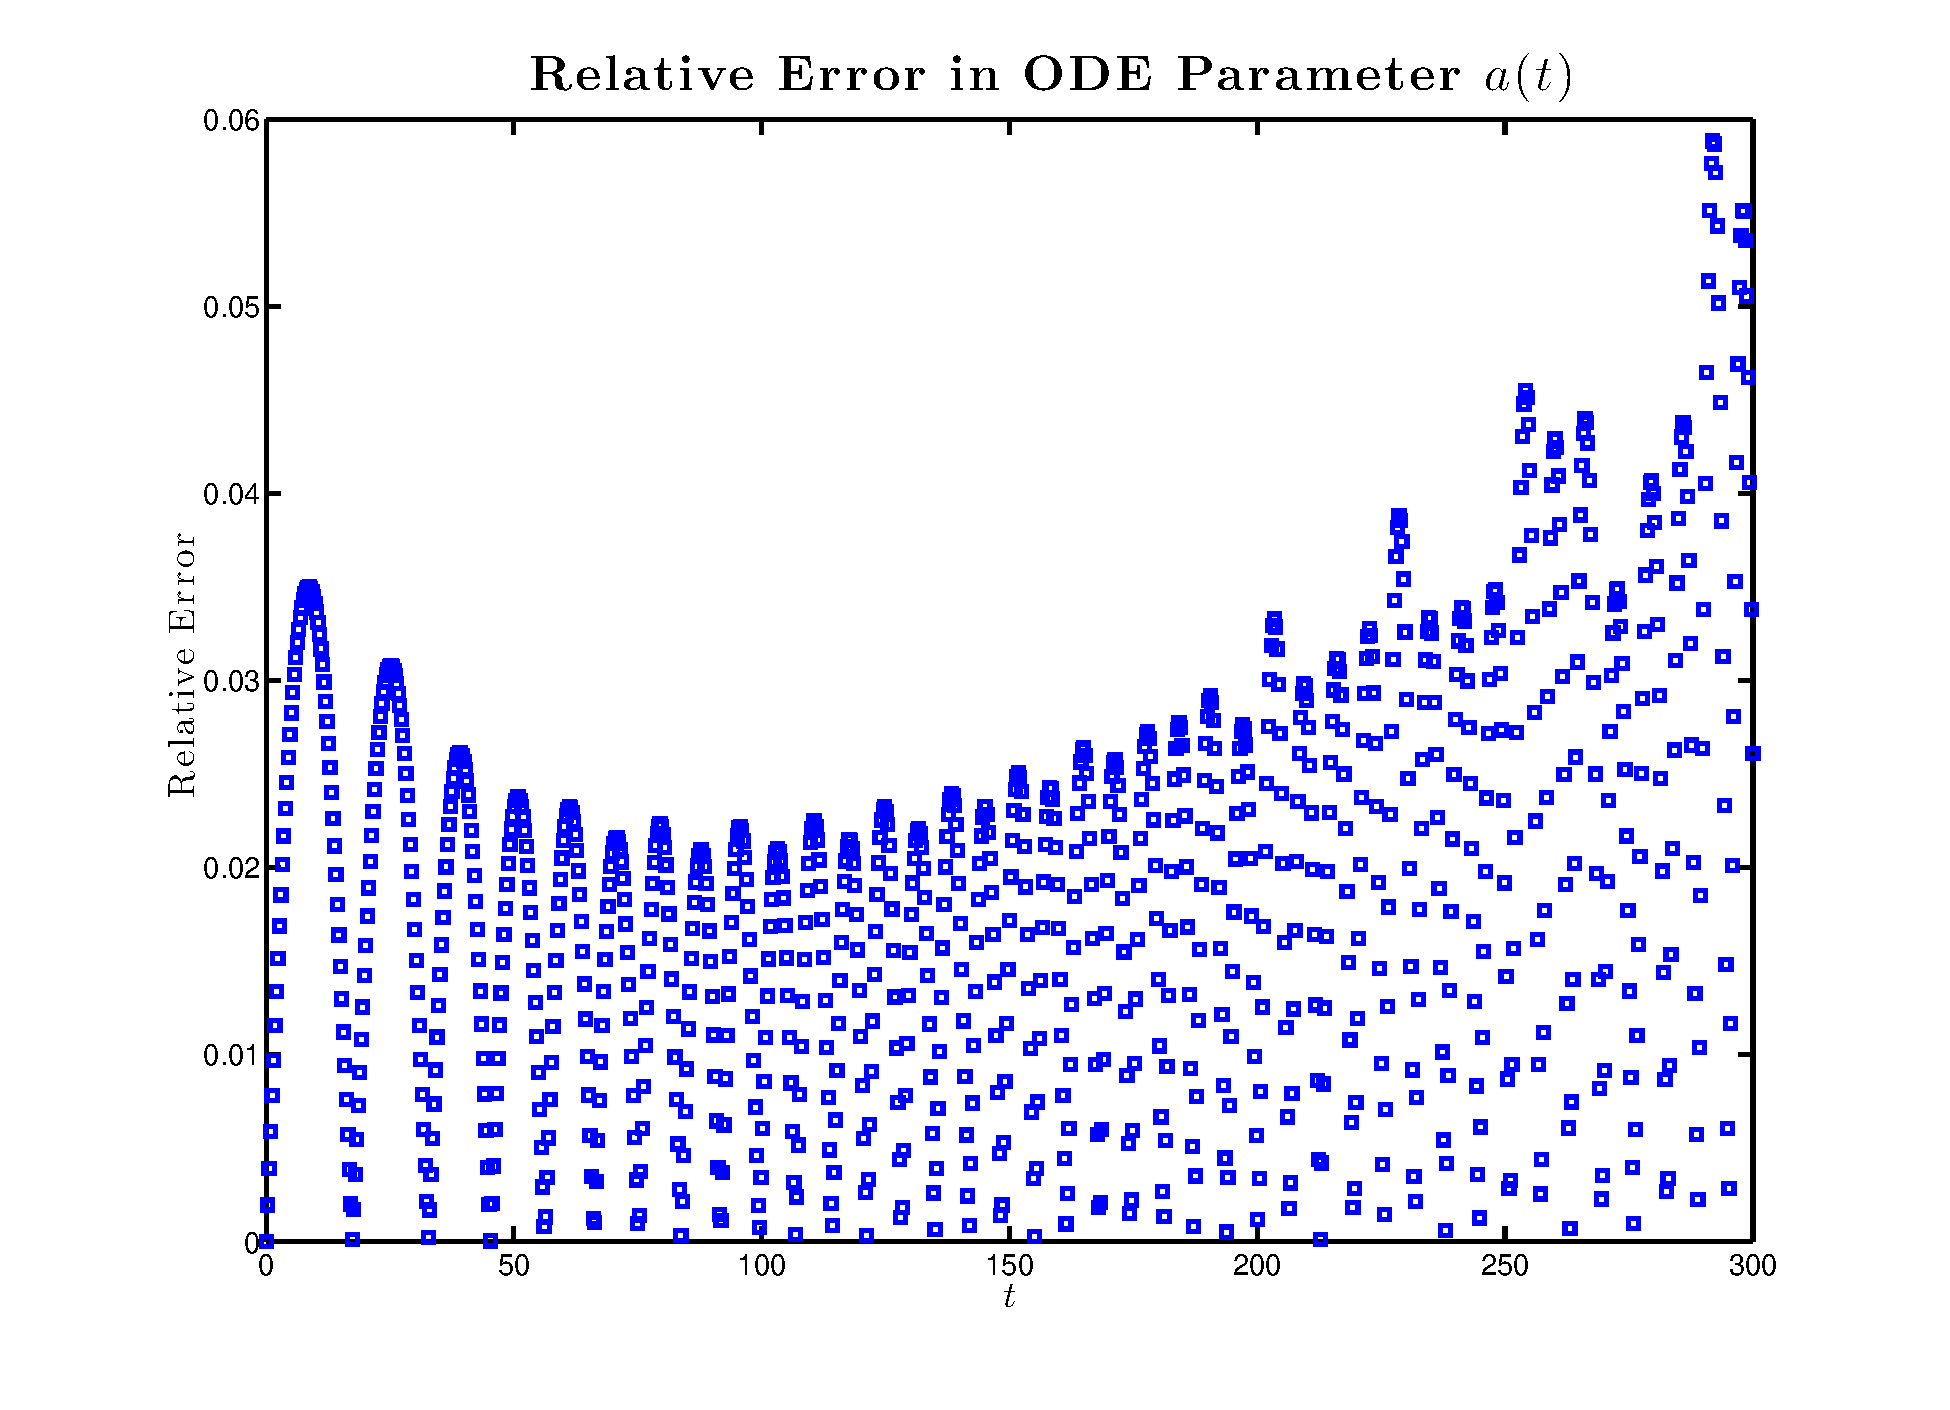
\includegraphics[width= \textwidth, height = \textwidth]{EPgainrelativeerror.eps}  
%	          \caption{Relative error between NCVA and PDE parameter $a(t)$ values for $a_0 = 0.5$.}
%	         \label{fig:PgainErr}
%	    \end{subfigure} 
%  \rule{35em}{0.5pt}
%   \caption[Relative Error in Amplitude for Exciton-Polariton Condensate: NLS with Linear Gain and Density Dependent Loss $\chi=(2/3) \sigma$]{{\bf Exciton-Polariton Condensate:} Amplitude parameter $a(t)$ relative error for $\chi=(2/3) \sigma$, $\sigma = 0.01$ where (A) $a_0 = 2$ and (B) $a_0=0.5$.}
%   \label{fig:Peq}
%\end{figure}

%\clearpage

%\begin{figure}[htbp]
%\centering
%\begin{subfigure}[t]{0.49\textwidth}
%  		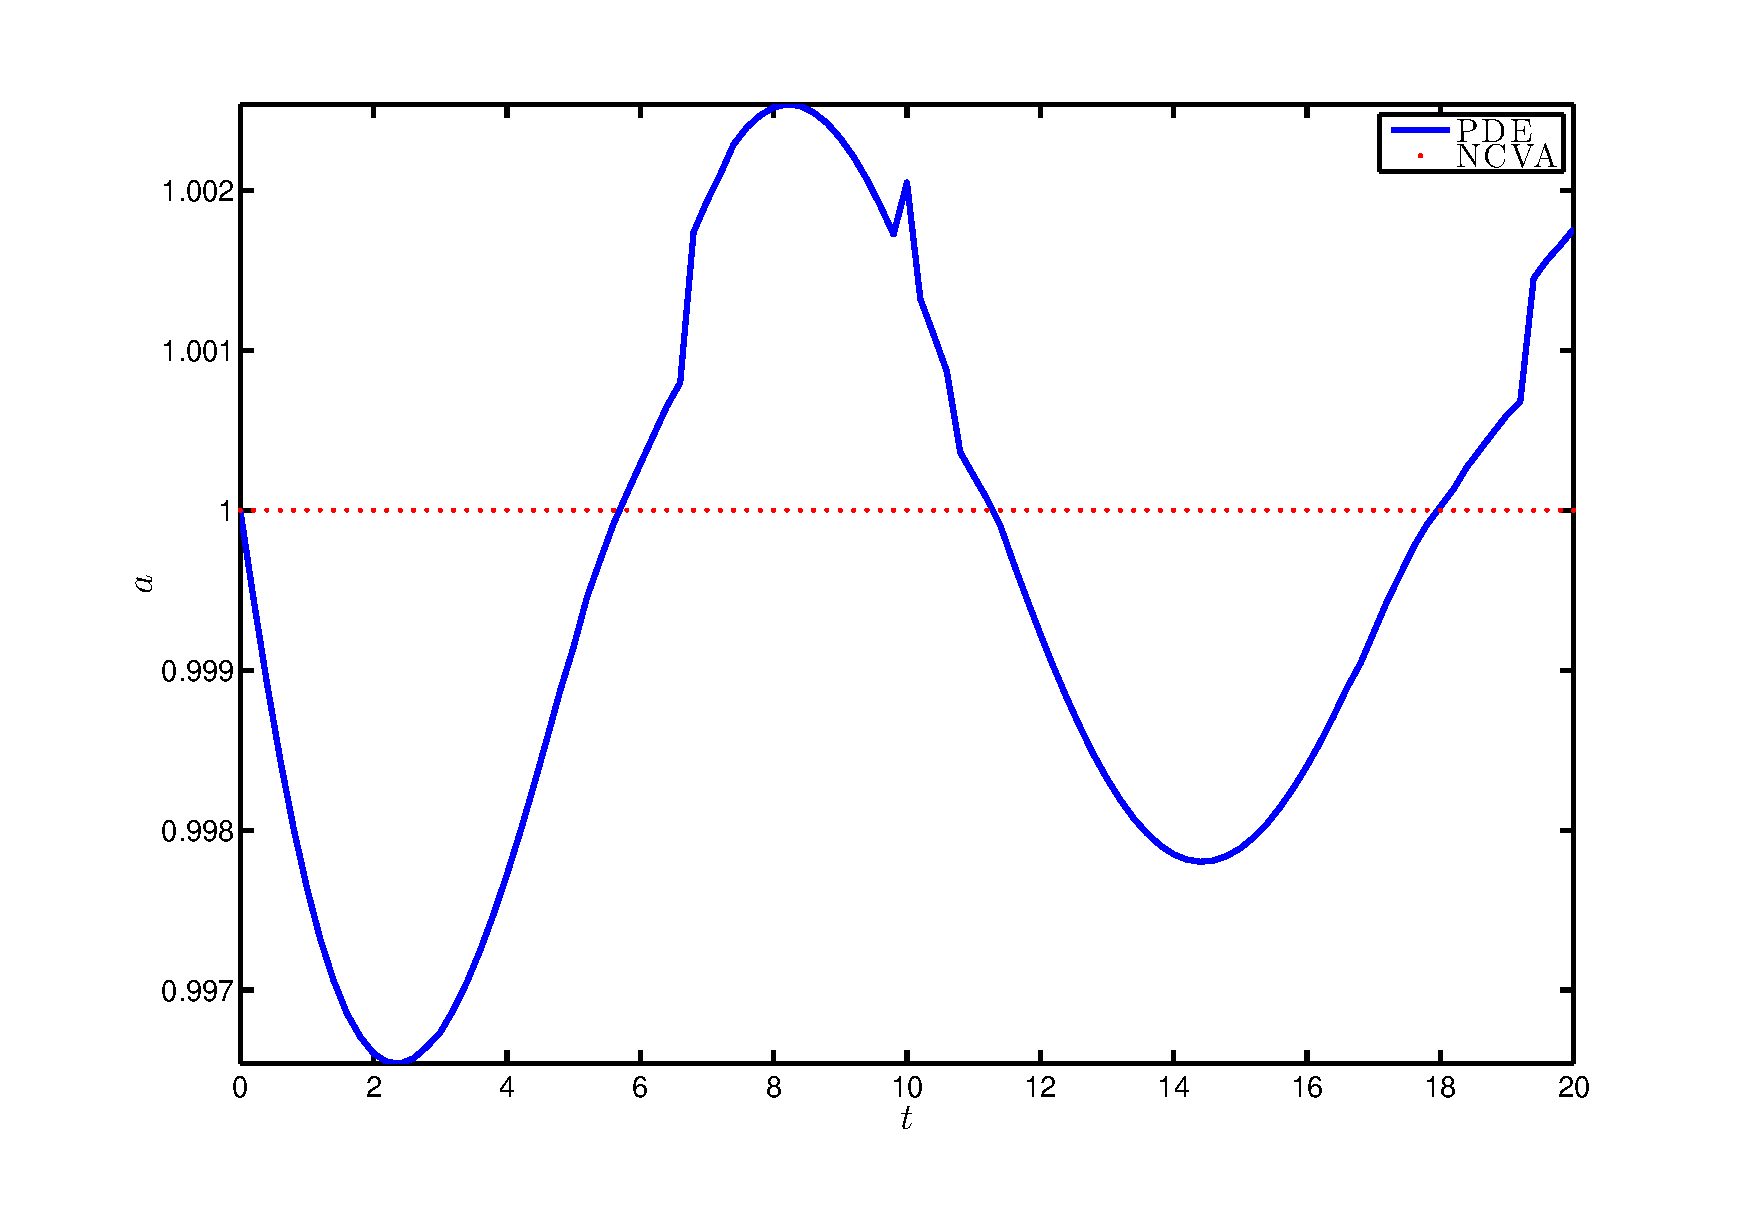
\includegraphics[width=\textwidth, height = \textwidth]{PE001a.eps}
%	         \caption{Amplitude parameter comparison $a(t)$ between PDE and NCVA solutions.}
%	         \label{fig:PLoss001a}
%	     \end{subfigure}
%  \begin{subfigure}[t]{0.49\textwidth}
%  		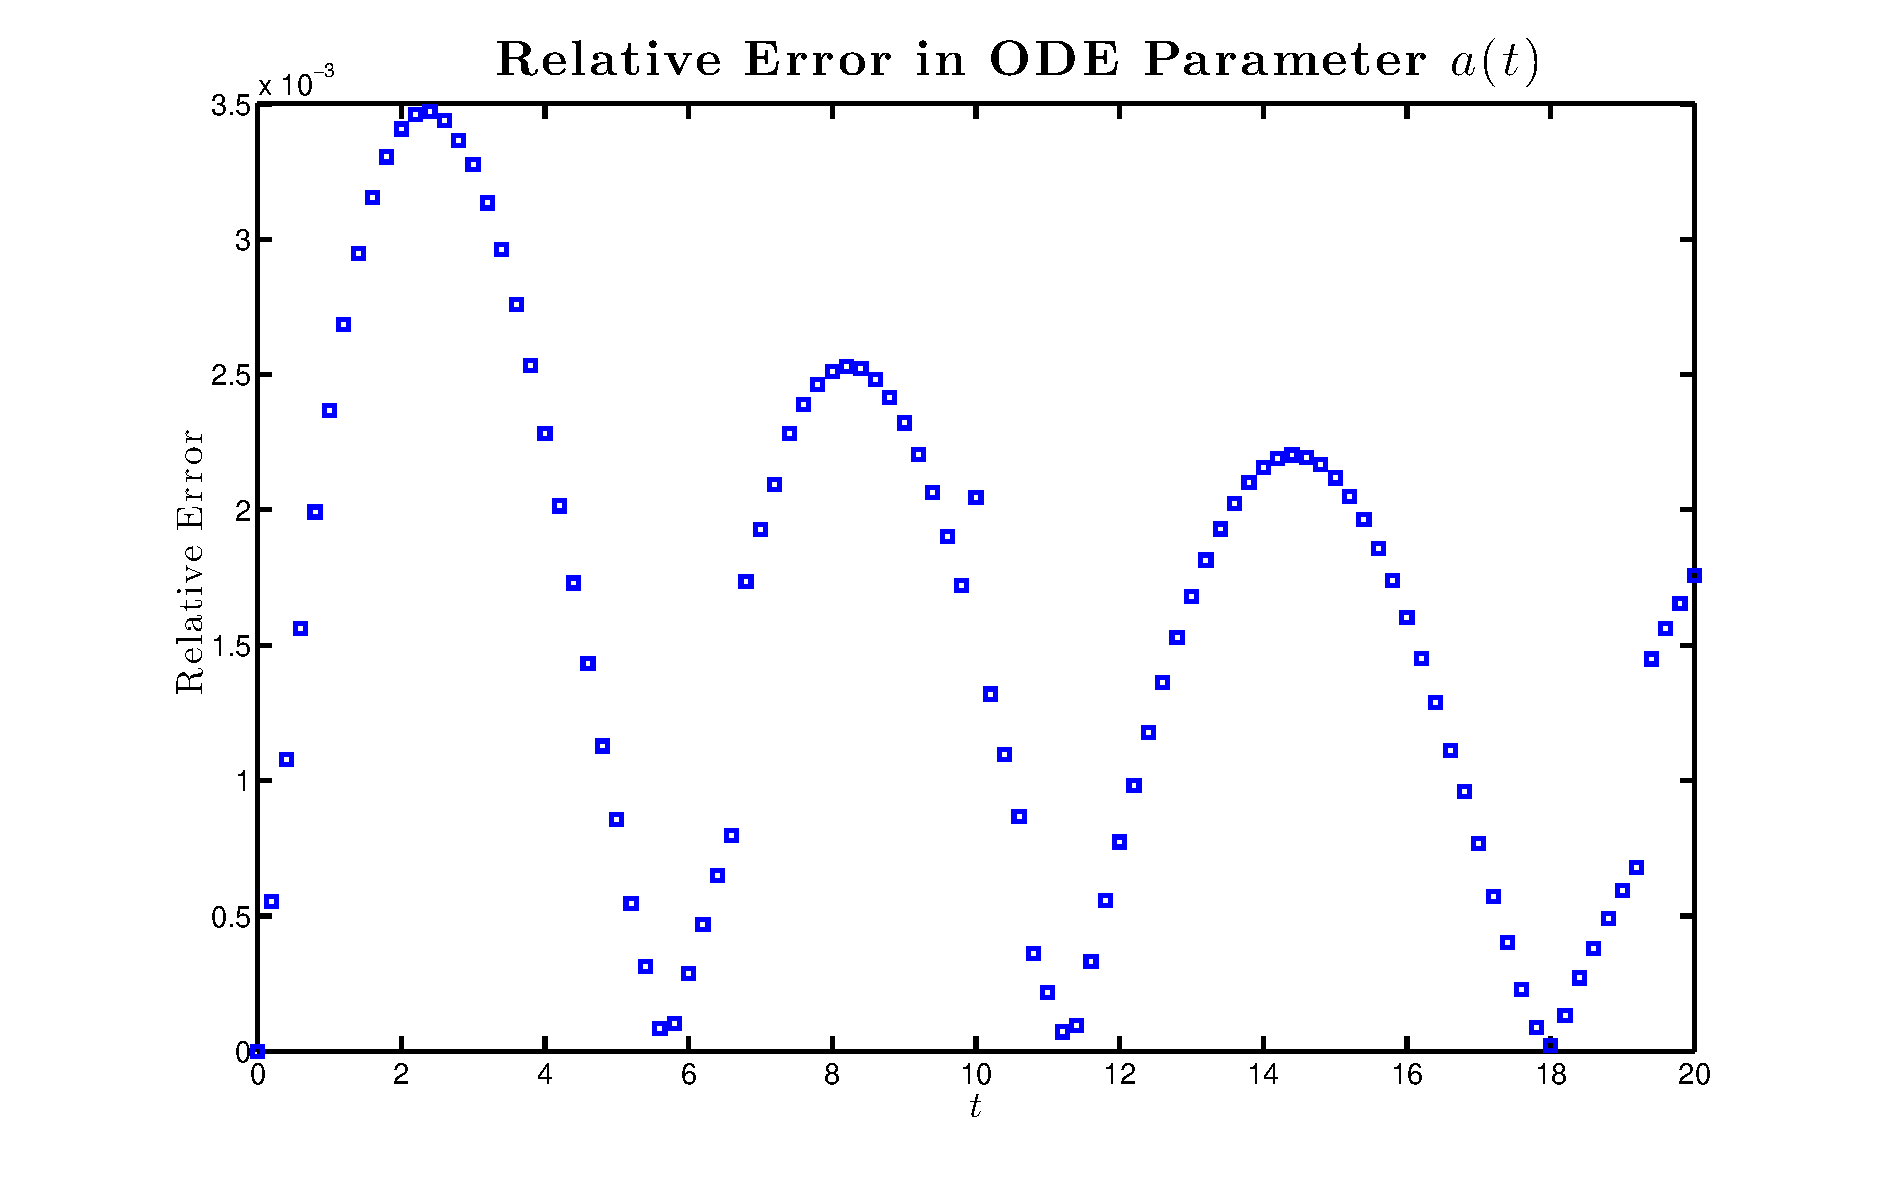
\includegraphics[width= \textwidth, height = \textwidth]{PE001relativeError.eps}  
%	          \caption{Relative error between NCVA and PDE parameter $a(t)$ values.}
%	         \label{fig:PLoss001Err}
%	    \end{subfigure} 
%  \rule{35em}{0.5pt}
%   \caption[Exciton-Polariton Condensate: NLS with Linear Gain $\sigma = 0.01$ and Density Dependent Loss $\chi=(2/3) \sigma$ Amplitude Comparison and Relative Error]{{\bf Exciton-Polariton Condensate:} Amplitude parameter $a(t)$ ansatz comparisons and relative error for  $\chi=2/3 \sigma$ and $\sigma = 0.01$.}
%   \label{fig:PlossA}
%\end{figure}
%
%
%\begin{figure}[htbp]
%\begin{subfigure}[b]{0.5\textwidth}
%  		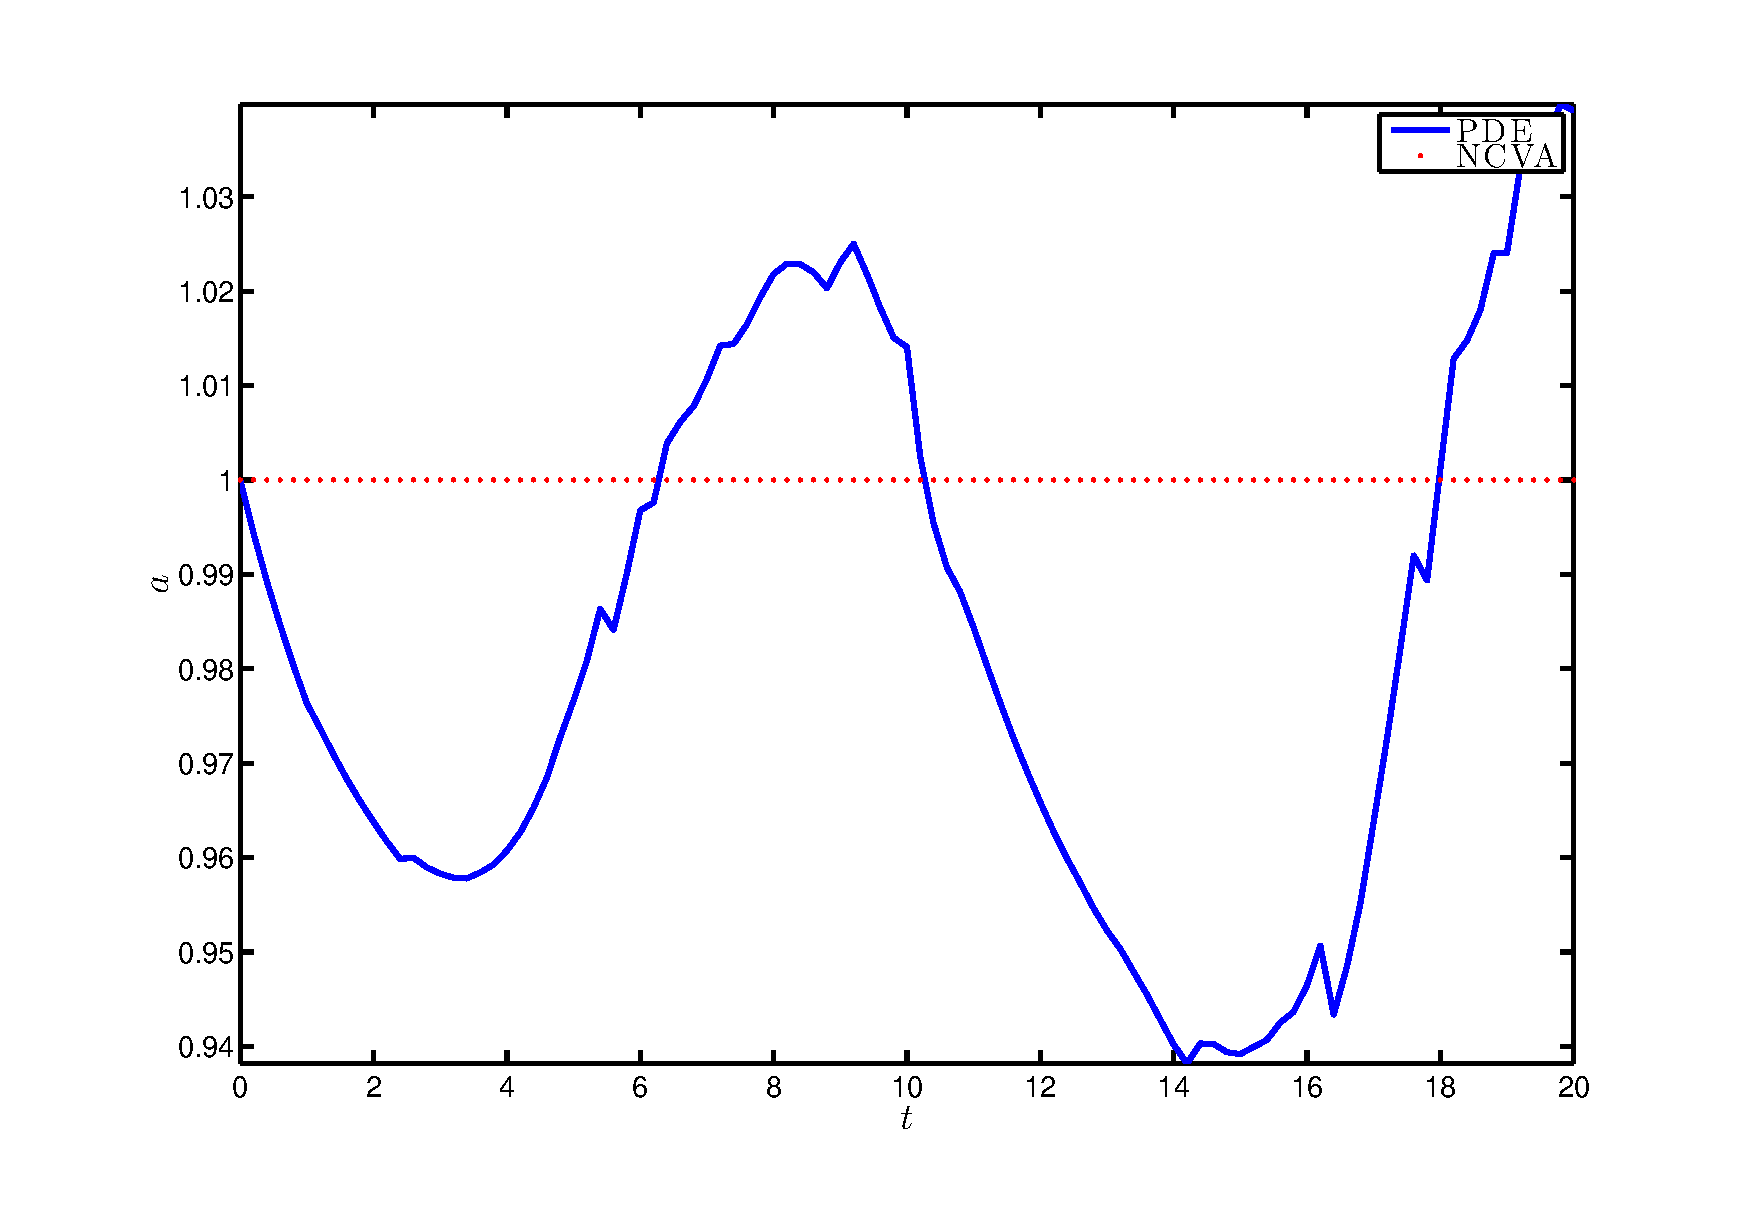
\includegraphics[width=\textwidth, height = \textwidth]{PE01a.eps}
%	         \caption{Amplitude parameter comparison $a(t)$ between PDE and NCVA solutions.}
%	         \label{fig:PLoss01a}
%	     \end{subfigure}
%  \begin{subfigure}[b]{0.5\textwidth}
%  		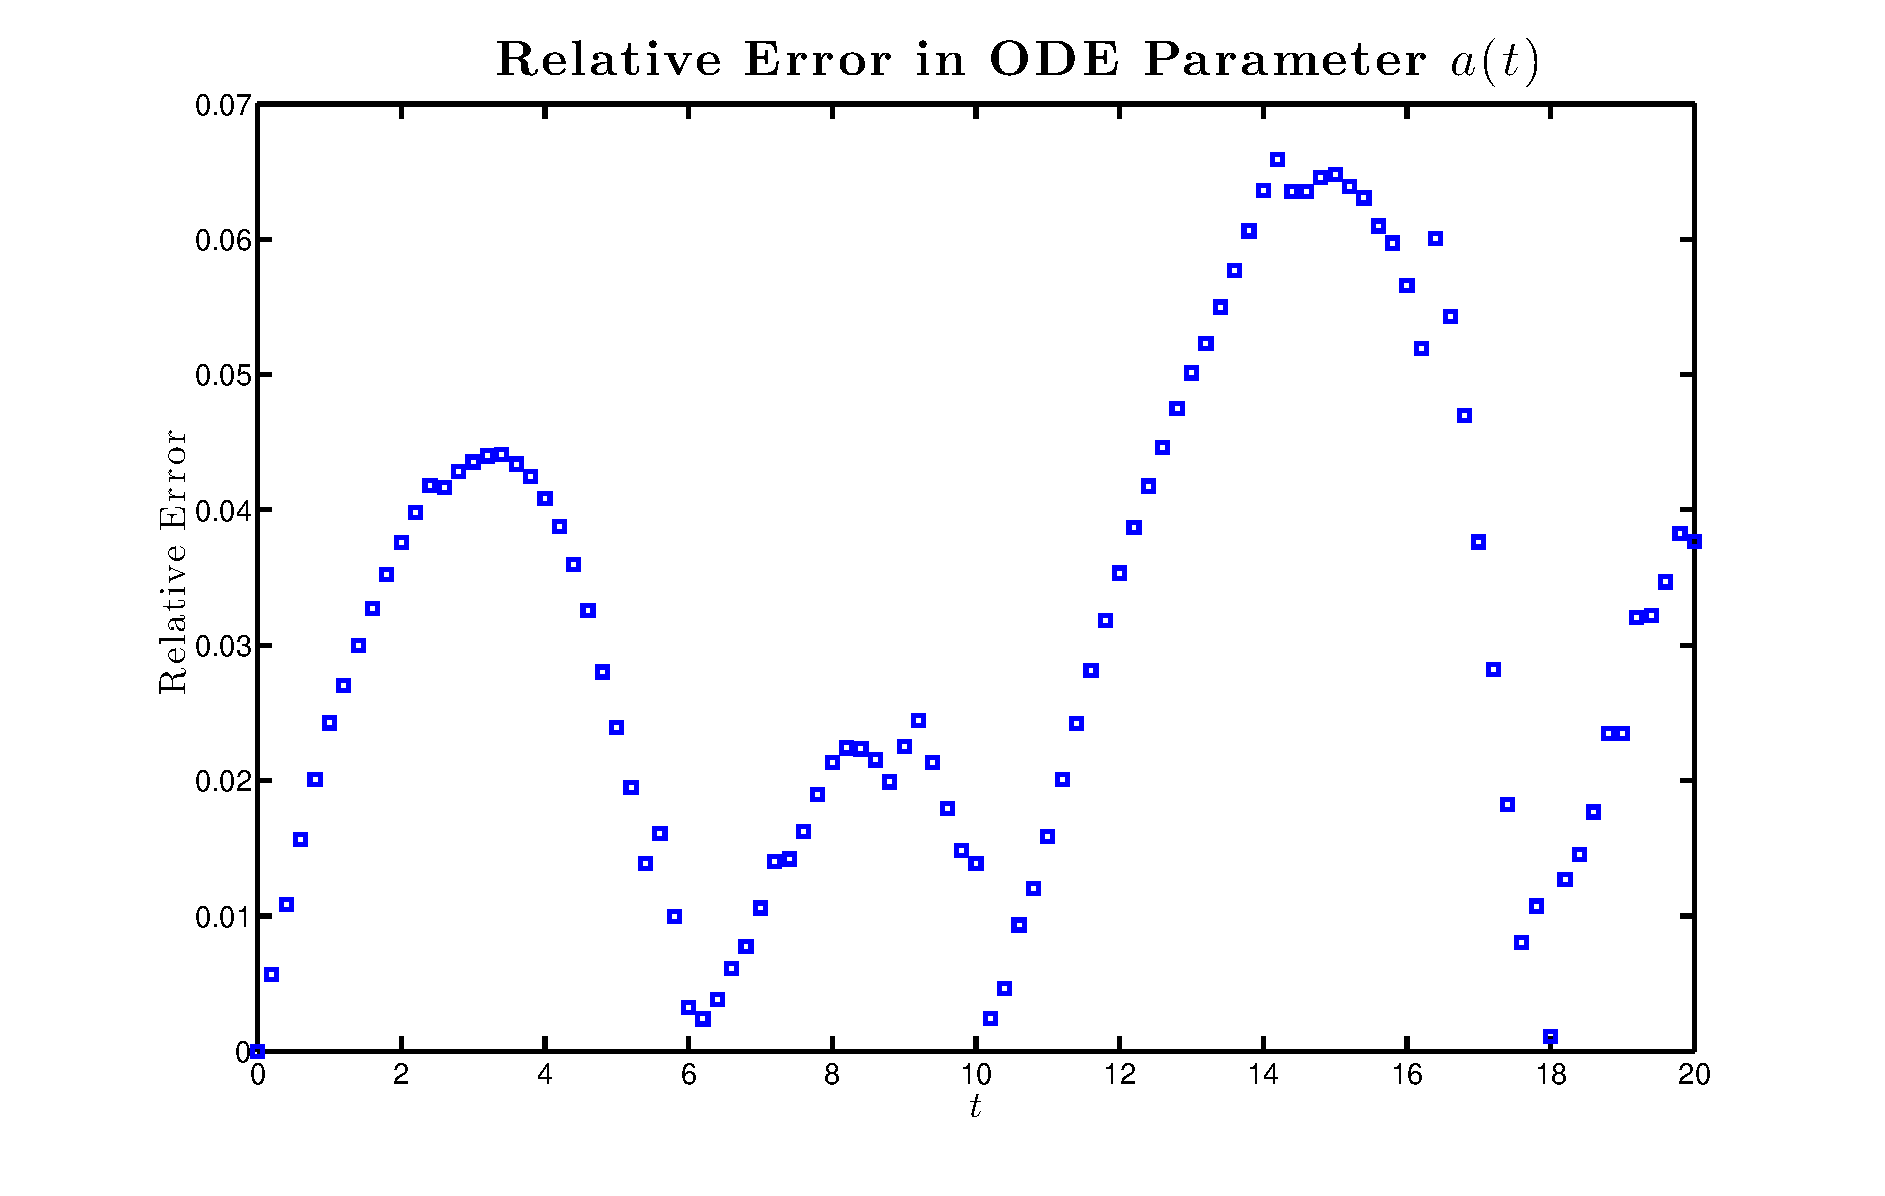
\includegraphics[width= \textwidth, height = \textwidth]{PE01relativeError.eps}  
%	          \caption{Relative error between NCVA and PDE parameter $a(t)$ values.}
%	         \label{fig:PLoss01Err}
%	    \end{subfigure} 
%  \rule{35em}{0.5pt}
%   \caption[Exciton-Polariton Condensate: NLS with Linear Gain $\sigma = 0.1$ and Density Dependent Loss $\chi=(2/3) \sigma$ Amplitude Comparison and Relative Error]{{\bf Exciton-Polariton Condensate:} Amplitude parameter $a(t)$ ansatz comparisons and relative error for  $\chi=2/3 \sigma$ and $\sigma = 0.1$.}
%   \label{fig:PlossA2}
%\end{figure}

\clearpage

